\documentclass[a4paper,twoside,10pt]{book}
% PAGE DIMENSIONS
% FOR A5 without scaling
%\usepackage[inner=18mm, outer=10mm,top=20mm,headsep=10mm,bottom=10mm,paperwidth=148mm,paperheight=210mm]{geometry}
% FOR 17x24cm
\usepackage[inner=30mm, outer=20mm,top=24mm,headsep=10mm,bottom=20mm,paperwidth=170mm,paperheight=240mm]{geometry}
% FOR A4
%\usepackage[inner=50mm, outer=40mm,top=60mm,headsep=10mm,bottom=57mm,paperwidth=210mm,paperheight=297mm]{geometry}
%\usepackage[inner=8.5mm, outer=12.5mm,top=10mm,headsep=5mm,bottom=10mm,paperwidth=141mm,paperheight=200mm]{geometry}
%\usepackage[inner=30mm, outer=23mm,top=29mm,headsep=10mm,bottom=23mm,paperwidth=210mm,paperheight=297mm]{geometry}
% FOR A5
%\usepackage[inner=25mm, outer=17mm,top=8mm,headsep=8mm,bottom=17mm,paperwidth=148mm,paperheight=210mm,includehead]{geometry}
% TABLES: full-width using X{10cm} column
\usepackage{tabularx}
% DRAWINGS (for chapter title)
\usepackage{tikz}
% TYPOGRAPHY: 
\usepackage[protrusion=true,final,factor=1500]{microtype}

% SOME extra math symbols
\usepackage{amssymb}




% CAPTIONS of figures/table styling
\usepackage[font={stretch=1.1,small},labelfont=bf]{caption} % order matters: stretch, then size
%\usepackage[font={small,sf},labelfont=bf]{caption} % small sans-serif + bold

% FONT  SIZES
\usepackage{fix-cm} % FOR ANY font sizes, not predefined
\renewcommand\footnotesize{\fontsize{7pt}{7pt}\selectfont}
\renewcommand\small{\fontsize{6pt}{6pt}\selectfont}
\renewcommand\normalsize{\fontsize{9pt}{9pt}\selectfont}
\renewcommand\large{\fontsize{10pt}{10pt}\selectfont}
\renewcommand\Large{\fontsize{11pt}{11pt}\selectfont}
\renewcommand\Huge{\fontsize{24pt}{24pt}\selectfont}

% LINE spacing
\renewcommand{\baselinestretch}{1.25}

% FONTS for LaTeX/XeLaTeX
\usepackage{ifxetex}
\ifxetex
			\usepackage{mathspec}
			\usepackage{polyglossia}
			\setdefaultlanguage[variant=uk]{english}
			\defaultfontfeatures{Ligatures=TeX} % To support LaTeX quoting style
			\setmainfont{Minion Pro} 
			\setsansfont{Myriad Pro}
			\setmathsfont(Digits,Greek,Latin)[Numbers={Proportional}]{Minion Pro}
			\setmathrm{Minion Pro}
			\usepackage[italic]{mathastext}
			%\setmainfont[BoldFont={SwiftNeueLTW01-Bold},ItalicFont={SwiftNeueLTW01-Italic}]{SwiftNeueLTW01} 
			%\setsansfont{UniversLTW01-55Roman}
\else
			%\usepackage[T1]{fontenc}
			%\usepackage[utf8]{inputenc}
			\usepackage[english]{babel}
			%\usepackage{fouriernc} % UTOPIA + FOURIER
			%\usepackage{mathpple} % palatino
			%\usepackage[sc]{mathpazo}
			\usepackage[charter]{mathdesign} %utopia, garamond
			\usepackage[scaled]{helvet}
			%\usepackage{newtxtt}
			\def\ttdefault{cmvtt}
			%\usepackage[light]{roboto}
			%\renewcommand{\sfdefault}{ua1}
\fi

\usepackage{hyperref}
% HEADER/FOOTER
\usepackage{fancyhdr}
\renewcommand{\headrulewidth}{0pt}
\renewcommand{\footrulewidth}{0pt}
\fancyhf{}
\makeatletter
	\let\ps@plain\ps@empty
\makeatother
% PLAIN: for first page of chapter
\fancypagestyle{plain}{
	\renewcommand{\headrulewidth}{0pt}
	\fancyhf{}
	\fancyhead[RO]{
		\makebox[2cm][l]{
			\makebox[4cm][c]{\normalsize
				\hskip0.25em\phantom{\thepage}\phantom{XX}~~$\left|\vphantom{\int_a^b}\right.$~~\thepage\phantom{XX}
			}
		}
	}
	\fancyhead[LE]{
		\makebox[2cm][r]{
			\makebox[4cm][c]{\normalsize
				\hskip0.45em\phantom{XX}\thepage~~$\left|\vphantom{\int_a^b}\right.$~~\phantom{XX}\phantom{\thepage}
			}
		}
	}
}
% REGULAR pages
\fancyhead[RO]{
	\makebox[2cm][l]{
		\makebox[4cm][c]{\normalsize
			\hskip0.25em\phantom{\thepage}\nouppercase\rightmark~~$\left|\vphantom{\int_a^b}\right.$~~\thepage\phantom{\nouppercase\rightmark}
		}
	}
}
\fancyhead[LE]{
	\makebox[2cm][r]{
		\makebox[4cm][c]{\normalsize
			\hskip0.45em\phantom{\nouppercase\leftmark}\thepage~~$\left|\vphantom{\int_a^b}\right.$~~\nouppercase\leftmark\phantom{\thepage}
		}
	}
}

% MARGIN labels, except chapter=0 (intro; conclusion; bibliography etc.)
% AND \setcouter{chapter}{0} has to be set explicitely in required chapters
\fancyfoot[RO]{
	\ifnum\value{chapter}>0
	\begin{tikzpicture}[remember picture, overlay]
	\node[rounded corners=2mm,inner sep=3mm,anchor=north east,black,fill=black!15,draw=black!75] at ([xshift=2mm,yshift=-\arabic{chapter}*1.3cm-1.1cm]current page.north east) {\fontsize{1cm}{1cm}\selectfont\thechapter};
	\end{tikzpicture}
	\fi
}
\fancyfoot[LE]{
	\ifnum\value{chapter}>0
	\begin{tikzpicture}[remember picture, overlay]
	\node[rounded corners=2mm,inner sep=3mm,anchor=north west,black,fill=black!15,draw=black!75] at ([xshift=-2mm,yshift=-\arabic{chapter}*1.3cm-1.1cm]current page.north west) {\fontsize{1cm}{1cm}\selectfont\thechapter};
	\end{tikzpicture}
	\fi
}



\pagestyle{fancy}
% HEADER contents - chapter name and section name
%\renewcommand{\chaptermark}[1]{\markboth{\thechapter.\, #1}{}}
\renewcommand{\chaptermark}[1]{\markboth{#1}{}}
\renewcommand{\sectionmark}[1]{\markright{\thesection.\, #1}}


% FLOATING objects
\usepackage{float}
% PICTURES
\usepackage{graphicx}
% NOT USED
\usepackage{setspace}

% SPACINGS in lists
\usepackage{enumitem}
% VERICAL: topsep partopsep parsep itemsep
% HORIZONTAL: leftmargin rightmargin listparindent labelwidth labelsep itemindent
% GLOBAL: \setlist[enumerate]{labelsep=*, leftmargin=1.5pc}
%\setlist{noitemsep}
\setlist{nosep}




% TABLES: nicer rulers
% AND nicer spacing between lines in tables
\usepackage{booktabs}
\renewcommand{\arraystretch}{1.2}


% TITLES styling
\usepackage[toctitles,explicit,raggedright]{titlesec}
\newcommand*\chapterlabel{}
% CHAPTER in frontmatter|backmatter
\titleformat{name=\chapter,numberless}[display]
	{\normalfont\rmfamily\Huge\bfseries}{}{1ex}
	{\flushright{\chapterlabel#1}}
% CHAPTER in mainmatter
\titleformat{\chapter}
{\gdef\chapterlabel{}\normalfont\rmfamily\Huge\bfseries}
{\gdef\chapterlabel{}}{-10em}
{
	\flushright{
		\begin{tikzpicture}
			%\draw[help lines,step=5mm] (0,-3) grid (-\linewidth,3);
			\node[black!50,anchor=east,inner sep=0mm] (a) at (0,0) {\fontsize{7cm}{8cm}\selectfont\thechapter};
			\begin{scope}[cm={1,0,-0.6,0.15,(0,0)}].
					\node[transform shape,black!30,anchor=south,inner sep=0mm] at (a.south) {\fontsize{7cm}{8cm}\selectfont{}\thechapter};
					%\node[transform shape,black!30,anchor=south east,inner sep=0mm] at (a.south) {\fontsize{3cm}{8cm}\selectfont{}\chaptername};
			\end{scope}
			\node[black!50,anchor=east,inner sep=0mm] (a) at (0,0) {\fontsize{7cm}{8cm}\selectfont\thechapter};
			\node[black!35,anchor=east,inner sep=0.20mm,scale=0.98] at (0,0) {\fontsize{7cm}{8cm}\selectfont\thechapter};
			\node[black!20,anchor=east,inner sep=0.40mm,scale=0.96] at (0,0) {\fontsize{7cm}{8cm}\selectfont\thechapter};
			%\node[black!20,scale=0.97] at (a) {\fontsize{6cm}{8cm}\selectfont\thechapter};
			%\node[anchor=east,black!45] at (0,-1) {\resizebox{\linewidth}{!}{\chaptername}};
			%\node[anchor=north east,inner sep=0mm] at (a.north east) {\parbox{\linewidth}{\raggedleft\chapterlabel#1}};
			\node[anchor=east,inner sep=0mm] at (0,0) {\parbox{\linewidth}{\raggedleft\chapterlabel#1}};
		\end{tikzpicture}
		%\chapterlabel#1
	}
}
% SPACING: chapter by default uses \@makechapterhead with extra spacing before and after the chapter title
\titlespacing*{\chapter}{0pt}{-25pt}{30pt}

%\titleformat{\section}[block]{\Large}{\bfseries\thesection.\,\,#1}{1em}{}
%\titleformat{\subsection}[block]{\large}{\bfseries\thesubsection.\,\,#1}{1em}{}
%\titleformat{\subsection}{\no}{\itshape\thesubsection.\,#1}{1em}{}


% GREEK letters in section/chapter titles AND in PDF bookmarks
%\usepackage[artemisia]{textgreek}




\usepackage{listings}
\definecolor{mygreen}{rgb}{0,0.6,0}
\definecolor{mygray}{rgb}{0.5,0.5,0.5}
\definecolor{mymauve}{rgb}{0.58,0,0.82}
\usepackage{amsmath}
\usepackage{pgfplots}

\lstset{ 
	backgroundcolor=\color{white},   % choose the background color; you must add \usepackage{color} or \usepackage{xcolor}; should come as last argument
	basicstyle=\small\ttfamily,
	belowcaptionskip=0em,        % the size of the fonts that are used for the code
	belowskip=-2em,
	breakatwhitespace=false,         % sets if automatic breaks should only happen at whitespace
	breaklines=true,                 % sets automatic line breaking
	captionpos=b,                    % sets the caption-position to bottom
	commentstyle=\color{mygreen},    % comment style
	deletekeywords={...},            % if you want to delete keywords from the given language
	escapeinside={\%*}{*)},          % if you want to add LaTeX within your code
	extendedchars=true,              % lets you use non-ASCII characters; for 8-bits encodings only, does not work with UTF-8
	frame=single,	                   % adds a frame around the code
	keepspaces=true,                 % keeps spaces in text, useful for keeping indentation of code (possibly needs columns=flexible)
	keywordstyle=\color{blue},       % keyword style
	language=Python,                 % the language of the code
	morekeywords={*,...},            % if you want to add more keywords to the set
	numbers=none,                    % where to put the line-numbers; possible values are (none, left, right)
	numbersep=5pt,                   % how far the line-numbers are from the code
	numberstyle=\tiny\color{mygray}, % the style that is used for the line-numbers
	rulecolor=\color{black},         % if not set, the frame-color may be changed on line-breaks within not-black text (e.g. comments (green here))
	showspaces=false,                % show spaces everywhere adding particular underscores; it overrides 'showstringspaces'
	showstringspaces=false,          % underline spaces within strings only
	showtabs=false,                  % show tabs within strings adding particular underscores
	stepnumber=2,                    % the step between two line-numbers. If it's 1, each line will be numbered
	stringstyle=\color{mymauve},     % string literal style
	tabsize=2,	                   % sets default tabsize to 2 spaces
	title=\lstname 			          % show the filename of files included with \lstinputlisting; also try caption instead of title
}
\def\inline{\lstinline[basicstyle=\ttfamily,keywordstyle={}]} %https://tex.stackexchange.com/questions/44702/can-you-change-lstinline-without-changing-the-global-lstset

% https://tex.stackexchange.com/questions/31085/is-there-a-standard-way-to-title-a-list-of-bullets
% name is purpose
\newenvironment{exercize}[1]{%
\vspace{0.2em}\noindent{\Large\textbf{#1}}
	\begin{itemize}}
	{\end{itemize}}
\begin{document}
\chapter{Improving the way neural networks learn}
\label{sec:3.1}
When a golf player is first learning to play golf, they usually spend most of their time developing a basic swing. Only gradually do they develop other shots, learning to chip, draw and fade the ball, building on and modifying their basic swing. In a similar way, up to now we've focused on understanding the backpropagation algorithm. It's our ``basic swing'', the foundation for learning in most work on neural networks. In this chapter I explain a suite of techniques which can be used to improve on our vanilla implementation of backpropagation, and so improve the way our networks learn.

The techniques we'll develop in this chapter include: a better choice of cost function, known as the cross-entropy cost function\ref{sec:3.1}; four so-called ``regularization'' methods (L1 and L2 regularization\ref{sec:3.2}, dropout, and artificial expansion of the training data), which make our networks better at generalizing beyond the training data; a better method for initializing the weights in the network\ref{sec:3.3}; and a set of heuristics to help choose good hyper-parameters for the network\ref{sec:3.5}. I'll also overview several other techniques in less depth\ref{sec:3.6}. The discussions are largely independent of one another, and so you may jump ahead if you wish. We'll also implement many of the techniques in running code\ref{sec:3.4}, and use them to improve the results obtained on the handwriting classification problem studied in Chapter 1.

Of course, we're only covering a few of the many, many techniques which have been developed for use in neural nets. The philosophy is that the best entree to the plethora of available techniques is in-depth study of a few of the most important. Mastering those important techniques is not just useful in its own right, but will also deepen your understanding of what problems can arise when you use neural networks. That will leave you well prepared to quickly pick up other techniques, as you need them.

\section{The cross-entropy cost function}
Most of us find it unpleasant to be wrong. Soon after beginning to learn the piano I gave my first performance before an audience. I was nervous, and began playing the piece an octave too low. I got confused, and couldn't continue until someone pointed out my error. I was very embarrassed. Yet while unpleasant, we also learn quickly when we're decisively wrong. You can bet that the next time I played before an audience I played in the correct octave! By contrast, we learn more slowly when our errors are less well-defined.

Ideally, we hope and expect that our neural networks will learn fast from their errors. Is this what happens in practice? To answer this question, let's look at a toy example. The example involves a neuron with just one input:

\begin{center}
	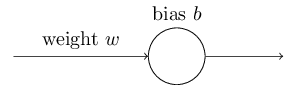
\includegraphics[width=0.5\linewidth]{figures/ch3/tikz28}
\end{center}
We'll train this neuron to do something ridiculously easy: take the input 1 to the output 0. Of course, this is such a trivial task that we could easily figure out an appropriate weight and bias by hand, without using a learning algorithm. However, it turns out to be illuminating to use gradient descent to attempt to learn a weight and bias. So let's take a look at how the neuron learns.

To make things definite, I'll pick the initial weight to be 0.6 and the initial bias to be 0.9. These are generic choices used as a place to begin learning, I wasn't picking them to be special in any way. The initial output from the neuron is 0.82, so quite a bit of learning will be needed before our neuron gets near the desired output, 0.0. 
%Click on ``Run'' in the bottom right corner below to see how the neuron learns an output much closer to 0.0. Note that this isn't a pre-recorded animation, your browser is actually computing the gradient, then using the gradient to update the weight and bias, and displaying the result.
The learning rate is $\eta$=0.15, which turns out to be slow enough that we can follow what's happening, but fast enough that we can get substantial learning in just a few seconds. The cost is the quadratic cost function, $C$, introduced back in Chapter 1. I'll remind you of the exact form of the cost function shortly, so there's no need to go and dig up the definition. %Note that you can run the animation multiple times by clicking on ``Run'' again.
\begin{center}%
	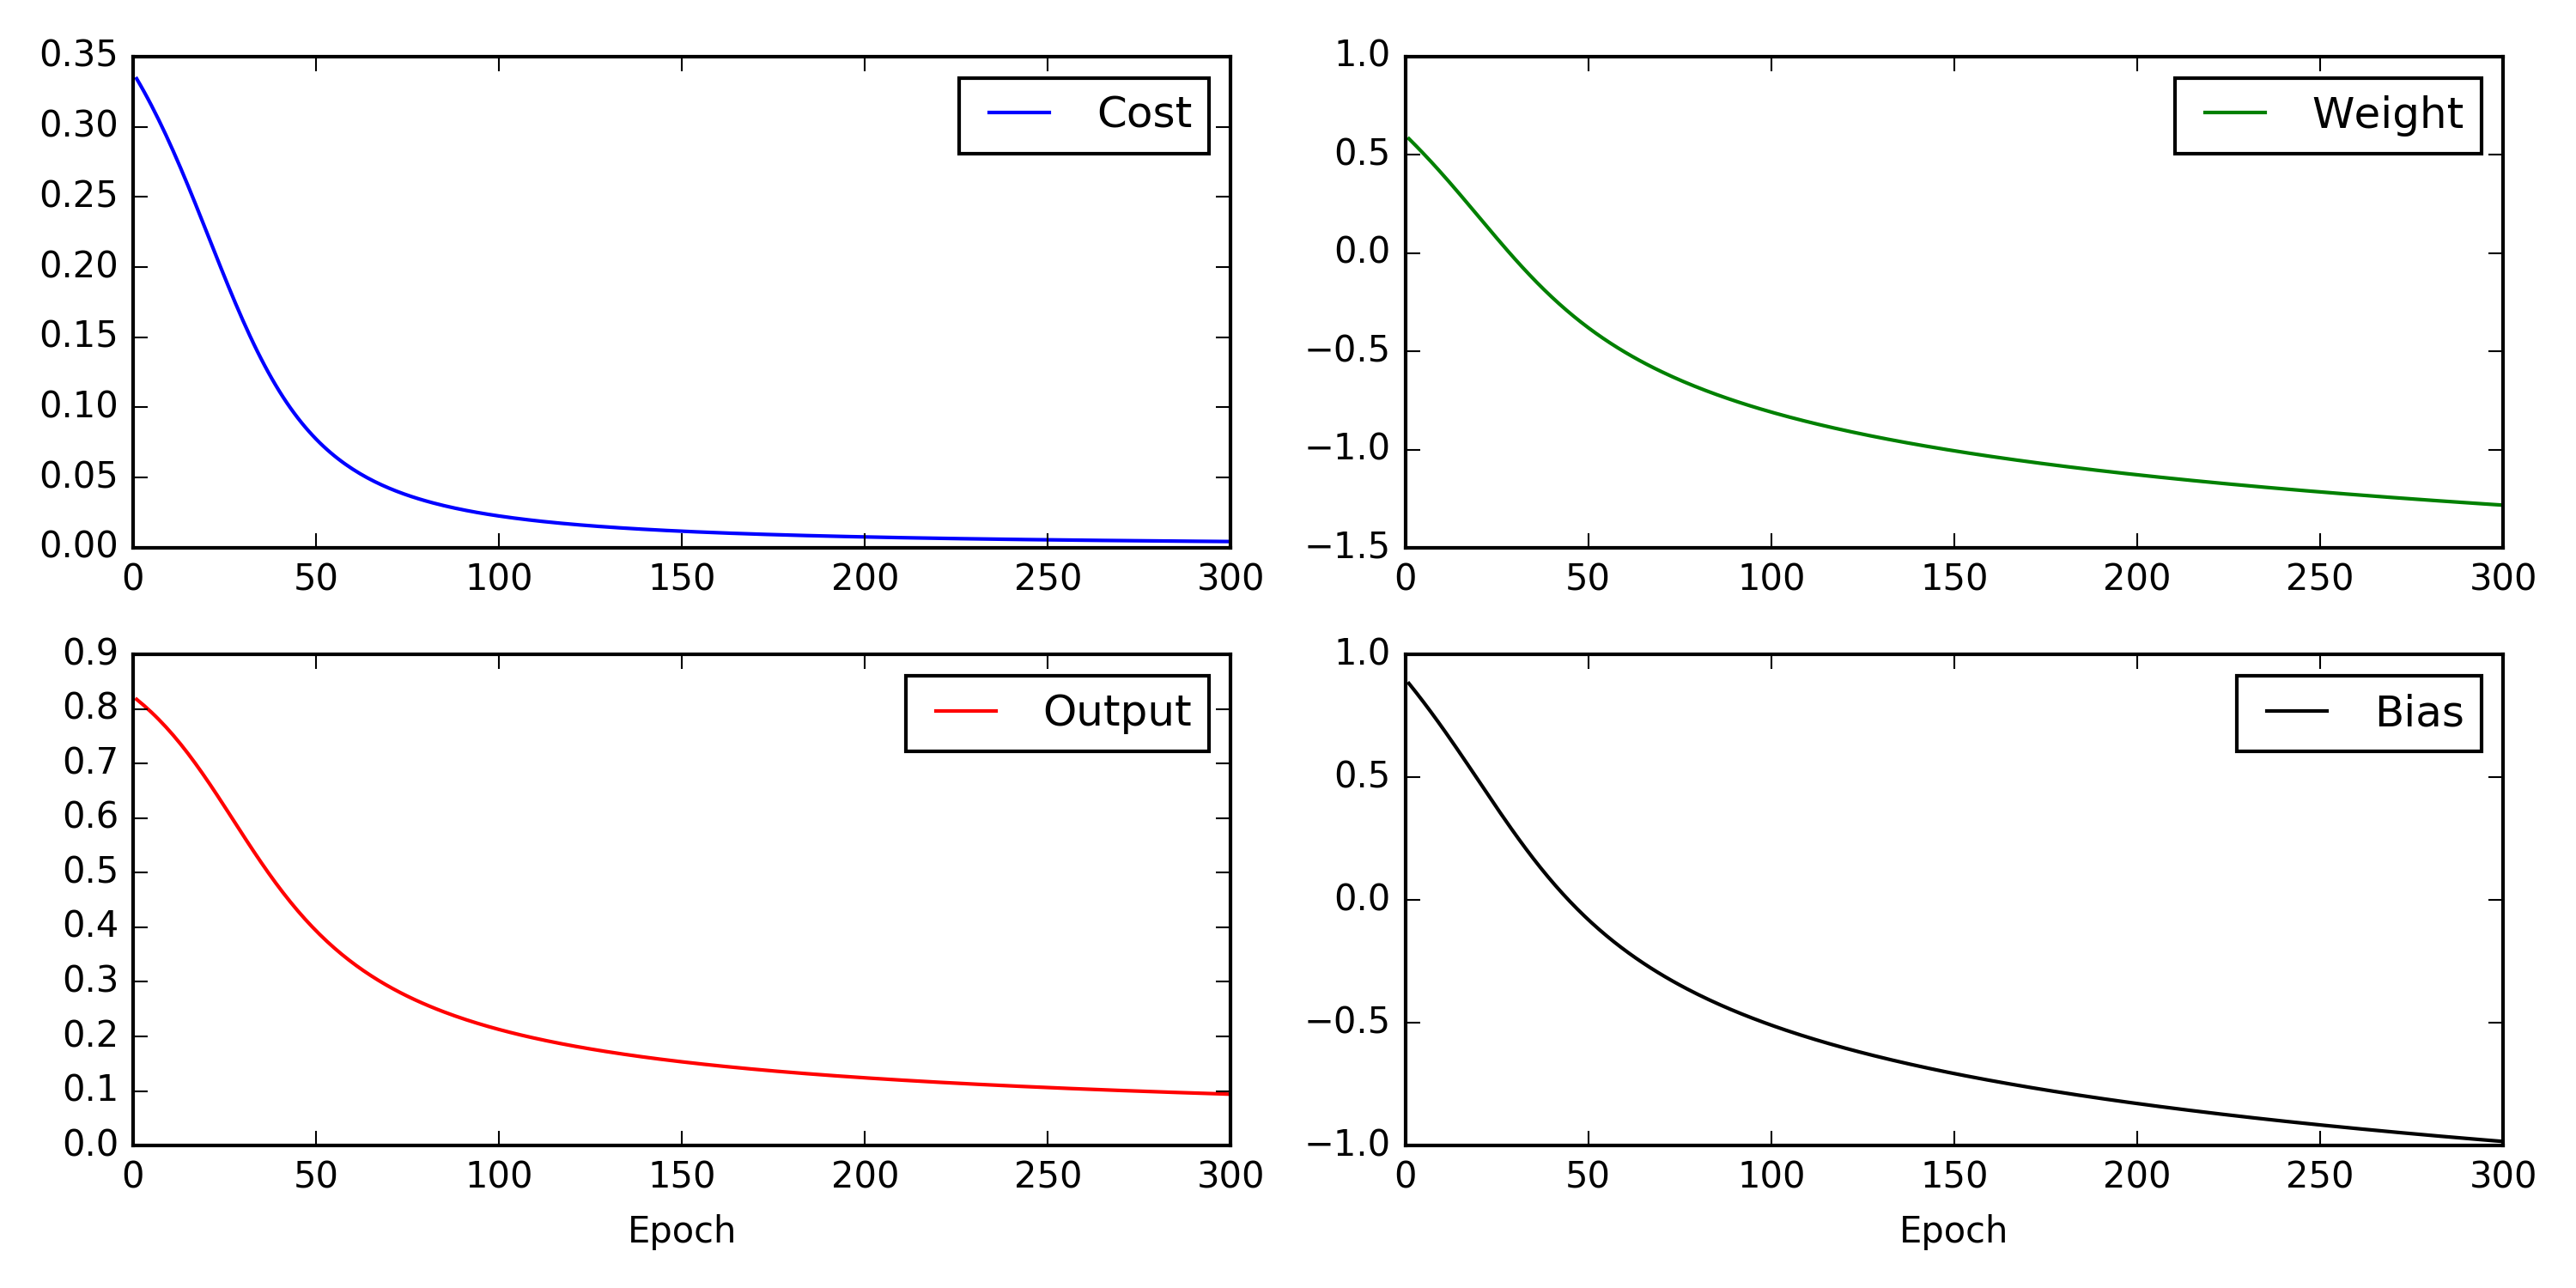
\includegraphics[width=0.75\linewidth]{./figures/ch3/animation_31}
\end{center}
As you can see, the neuron rapidly learns a weight and bias that drives down the cost, and gives an output from the neuron of about 0.09. That's not quite the desired output, 0.0, but it is pretty good. Suppose, however, that we instead choose both the starting weight and the starting bias to be 2.0. In this case the initial output is 0.98, which is very badly wrong. Let's look at how the neuron learns to output 0 in this case. %Click on ``Run'' again:
\begin{center}%
	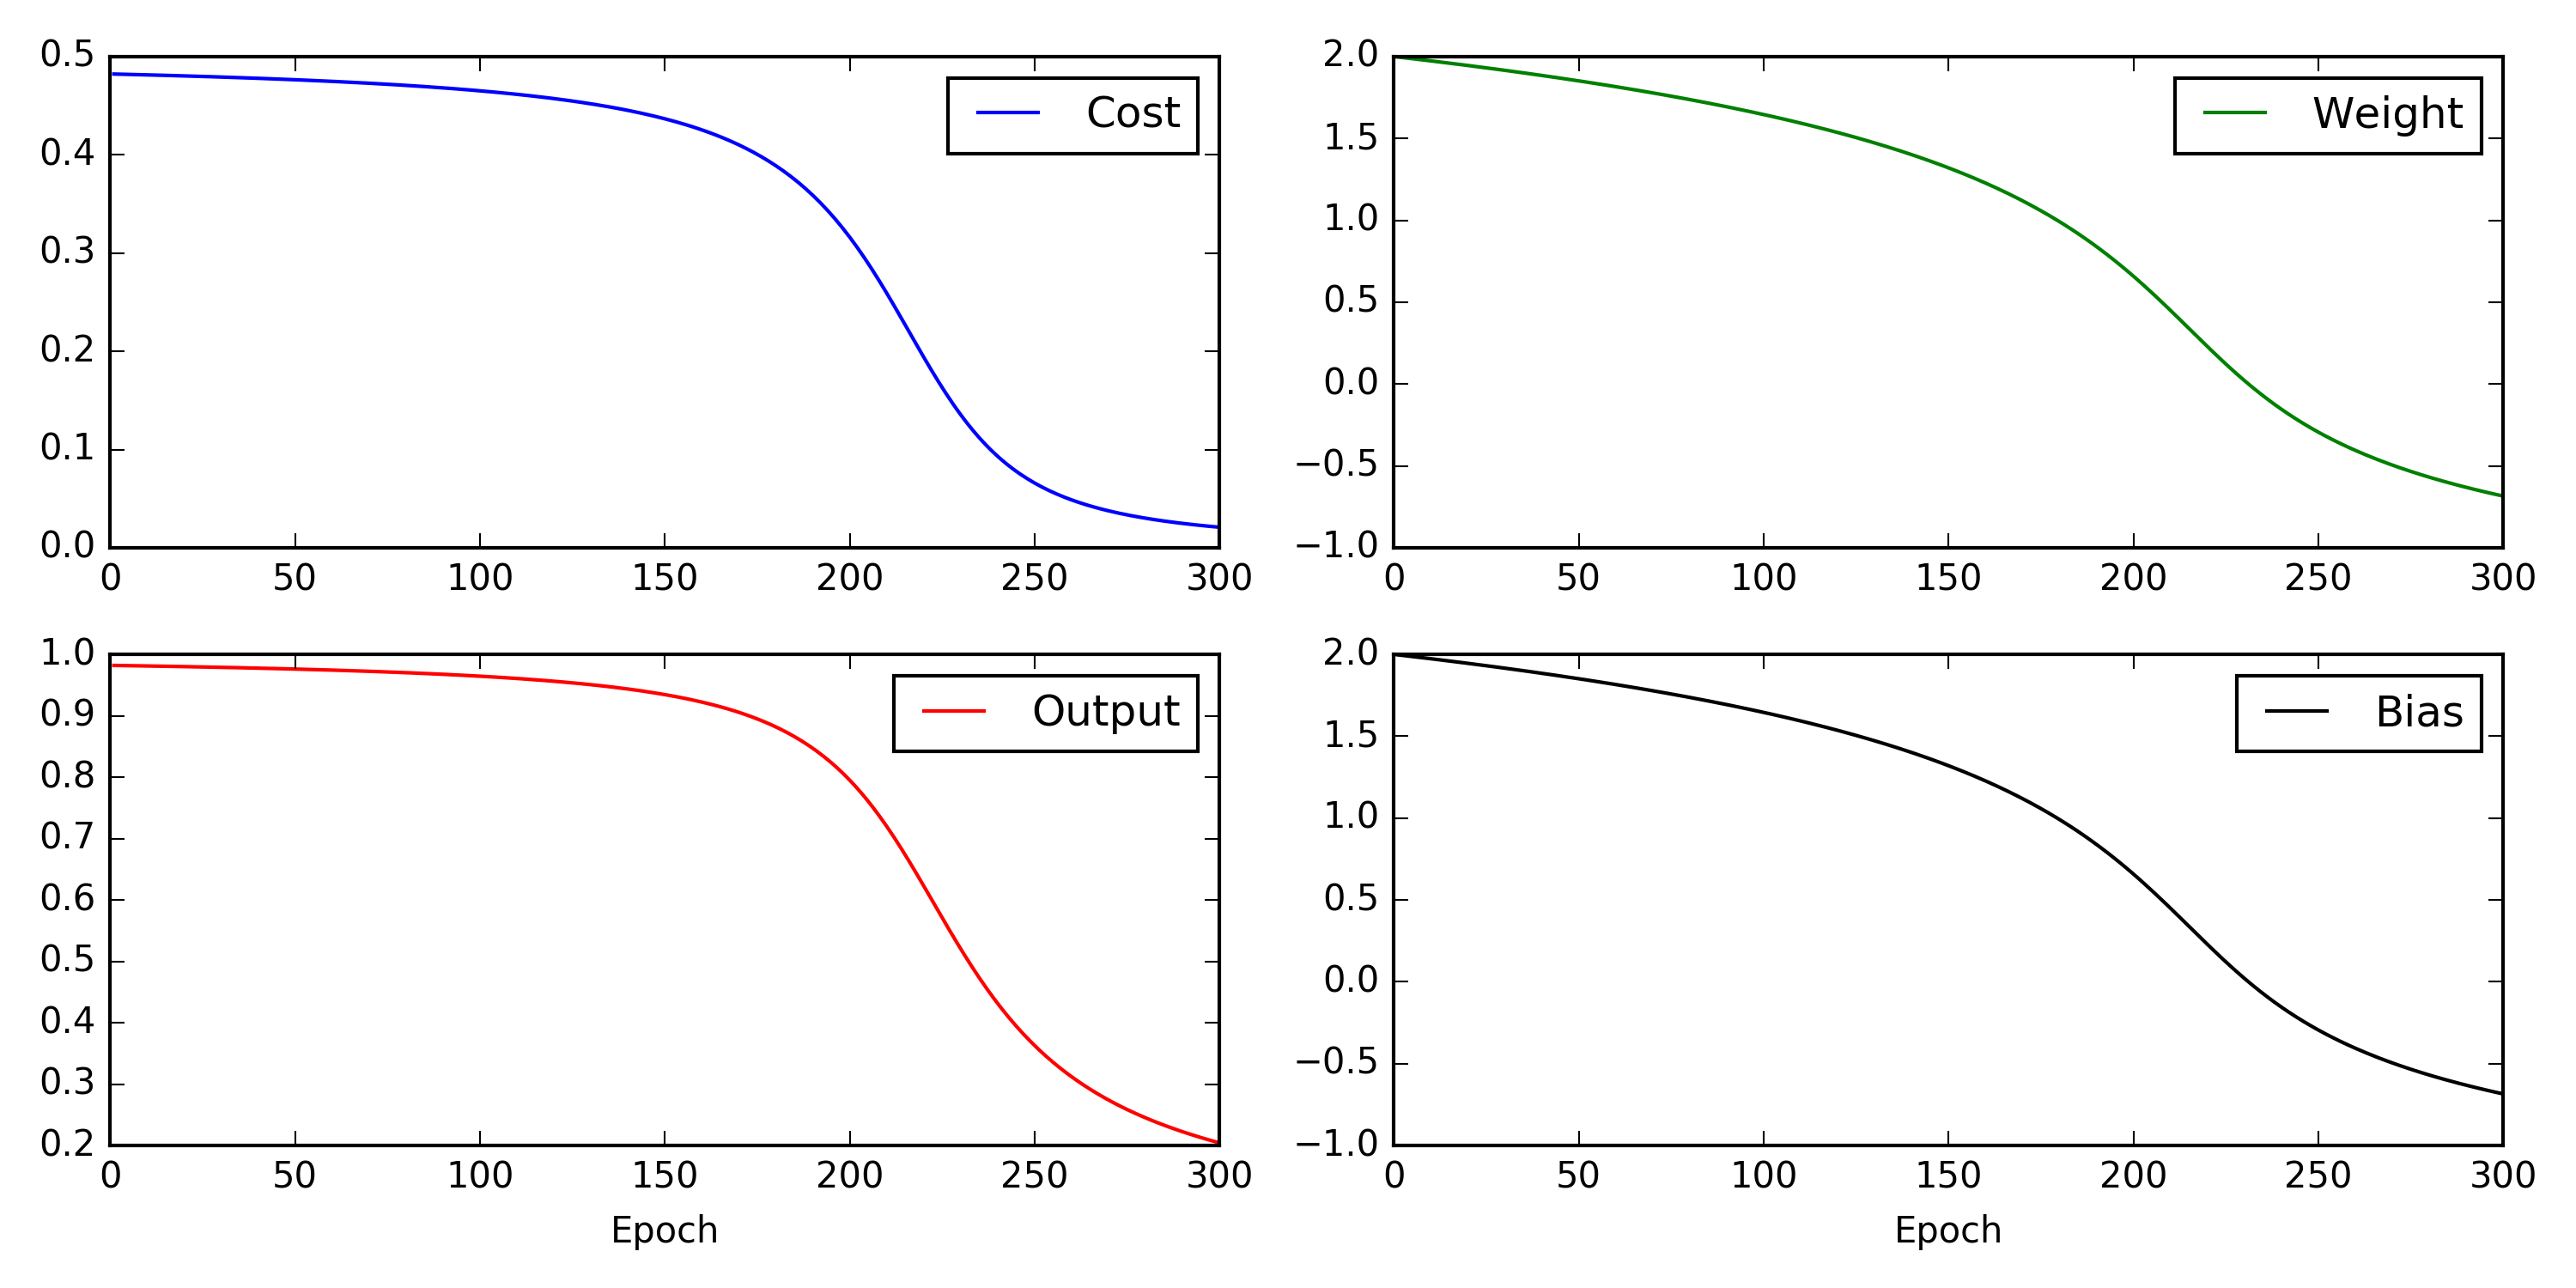
\includegraphics[width=0.75\linewidth]{./figures/ch3/animation_32}
\end{center}
Although this example uses the same learning rate ($\eta=0.15$), we can see that learning starts out much more slowly. Indeed, for the first 150 or so learning epochs, the weights and biases don't change much at all. Then the learning kicks in and, much as in our first example, the neuron's output rapidly moves closer to 0.0.

This behavior is strange when contrasted to human learning. As I said at the beginning of this section, we often learn fastest when we're badly wrong about something. But we've just seen that our artificial neuron has a lot of difficulty learning when it's badly wrong -- far more difficulty than when it's just a little wrong. What's more, it turns out that this behavior occurs not just in this toy model, but in more general networks. Why is learning so slow? And can we find a way of avoiding this slowdown?

To understand the origin of the problem, consider that our neuron learns by changing the weight and bias at a rate determined by the partial derivatives of the cost function, $\partial{}C/\partial{}w$ and $\partial{}C/\partial{}b$. So saying ``learning is slow'' is really the same as saying that those partial derivatives are small. The challenge is to understand why they are small. To understand that, let's compute the partial derivatives. Recall that we're using the quadratic cost function, which, from Equation \ref{eq:6}, is given by
\begin{equation}
C = \frac{(y-a)^2}2,\label{eq:54}
\end{equation}
where $a$ is the neuron's output when the training input $x=1$ is used, and $y=0$ is the corresponding desired output. To write this more explicitly in terms of the weight and bias, recall that $a=\sigma{}(z)$, where $z=wx+b$. Using the chain rule to differentiate with respect to the weight and bias we get
\begin{eqnarray} 
\frac{\partial C}{\partial w} & = & (a-y)\sigma'(z) x = a \sigma'(z) \label{eq:55}\\
\frac{\partial C}{\partial b} & = & (a-y)\sigma'(z) = a \sigma'(z),
\label{eq:56}
\end{eqnarray}
where I have substituted $x=1$ and $y=0$. To understand the behavior of these expressions, let's look more closely at the $\sigma{}'(z)$ term on the right-hand side. Recall the shape of the $\sigma{}$ function:
\begin{center}
\begin{tikzpicture}[scale=0.75]
\begin{axis}[title={Sigmoid function}]
\addplot[blue,domain=-5:5,samples=81]{1/(1+exp(-x)};
\end{axis}
\end{tikzpicture}
\end{center}
We can see from this graph that when the neuron's output is close to 1, the curve gets very flat, and so $\sigma{}'(z)$ gets very small. Equations \ref{eq:55} and \ref{eq:56} then tell us that $\partial{}C/\partial{}w$ and $\partial{}C/\partial{}b$ get very small. This is the origin of the learning slowdown. What's more, as we shall see a little later, the learning slowdown occurs for essentially the same reason in more general neural networks, not just the toy example we've been playing with.

\subsection{Introducing the cross-entropy cost function}
How can we address the learning slowdown? It turns out that we can solve the problem by replacing the quadratic cost with a different cost function, known as the cross-entropy. To understand the cross-entropy, let's move a little away from our super-simple toy model. We'll suppose instead that we're trying to train a neuron with several input variables, $x_1,x_2,\ldots$, corresponding weights $w_1,w_2,\ldots$, and a bias, $b$:
\begin{center}
	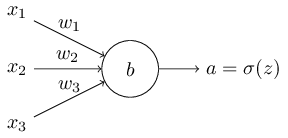
\includegraphics[scale=0.5]{./figures/ch3/tikz29}
\end{center}
The output from the neuron is, of course, $a=\sigma(z)$, where $z=\sum_jw_jb_j+b$ is the weighted sum of the inputs. We define the cross-entropy cost function for this neuron by
%C=-1n∑x[ylna+(1-y)ln(1-a)],(57)
\begin{equation}
	C = -\frac{1}{n} \sum_x \left[y \ln a + (1-y ) \ln (1-a) \right],
	\label{eq:57}
\end{equation}
where $n$ is the total number of items of training data, the sum is over all training inputs, $x$, and $y$ is the corresponding desired output.

It's not obvious that the expression (\ref{eq:57}) fixes the learning slowdown problem. In fact, frankly, it's not even obvious that it makes sense to call this a cost function! Before addressing the learning slowdown, let's see in what sense the cross-entropy can be interpreted as a cost function.

Two properties in particular make it reasonable to interpret the cross-entropy as a cost function. First, it's non-negative, that is, $C>0$. To see this, notice that: (a)~all the individual terms in the sum in (\ref{eq:57}) are negative, since both logarithms are of numbers in the range 0 to 1; and (b)~there is a minus sign out the front of the sum.

Second, if the neuron's actual output is close to the desired output for all training inputs, x, then the cross-entropy will be close to zero\footnote{To prove this I will need to assume that the desired outputs y are all either 0 or 1. This is usually the case when solving classification problems, for example, or when computing Boolean functions. To understand what happens when we don't make this assumption, see the exercises at the end of this section.}. To see this, suppose for example that $y=0$ and $a\approx0$ for some input $x$. This is a case when the neuron is doing a good job on that input. We see that the first term in the expression (57) for the cost vanishes, since $y=0$, while the second term is just $-\ln(1-a)\approx0$. A similar analysis holds when $y=1$ and $a\approx1$. And so the contribution to the cost will be low provided the actual output is close to the desired output.

Summing up, the cross-entropy is positive, and tends toward zero as the neuron gets better at computing the desired output, $y$, for all training inputs, $x$. These are both properties we'd intuitively expect for a cost function. Indeed, both properties are also satisfied by the quadratic cost. So that's good news for the cross-entropy. But the cross-entropy cost function has the benefit that, unlike the quadratic cost, it avoids the problem of learning slowing down. To see this, let's compute the partial derivative of the cross-entropy cost with respect to the weights. We substitute $a=\sigma(z)$ into (\ref{eq:57}), and apply the chain rule twice, obtaining:
%\partial{}C\partial{}wj==-1n∑x(y\sigma(z)-(1-y)1-\sigma(z))\partial{}\sigma\partial{}wj-1n∑x(y\sigma(z)-(1-y)1-\sigma(z))\sigma'(z)x_j.(58)(59)
\begin{equation}
	\frac{\partial C}{\partial w_j}  =  -\frac{1}{n} \sum_x \left(
	\frac{y }{\sigma(z)} -\frac{(1-y)}{1-\sigma(z)} \right)
	\frac{\partial \sigma}{\partial w_j} = 
 -\frac{1}{n} \sum_x \left( 
	\frac{y}{\sigma(z)} 
	-\frac{(1-y)}{1-\sigma(z)} \right)\sigma'(z) x_j.
	\label{eq:59}
\end{equation}Putting everything over a common denominator and simplifying this becomes:
\begin{equation}
	\frac{\partial C}{\partial w_j}  =  \frac{1}{n}
	\sum_x \frac{\sigma'(z) x_j}{\sigma(z) (1-\sigma(z))}
	(\sigma(z)-y).
	\label{eq:60}
\end{equation}
%\partial{}C\partial{}wj=1n∑x\sigma'(z)x_j\sigma(z)(1-\sigma(z))(\sigma(z)-y).(60)
Using the definition of the sigmoid function, $\sigma(z)=1/(1+e^{-z})$, and a little algebra we can show that $\sigma'(z)=\sigma(z)(1-\sigma(z))$. I'll ask you to verify this in an exercise below, but for now let's accept it as given. We see that the $\sigma'(z)$ and $\sigma(z)(1-\sigma(z))$ terms cancel in the equation just above, and it simplifies to become:
%\partial{}C\partial{}wj=1n∑xx_j(\sigma(z)-y).(61)
\begin{equation}
	\frac{\partial C}{\partial w_j} =  \frac{1}{n} \sum_x x_j(\sigma(z)-y).
	\label{eq:61}
\end{equation}
This is a beautiful expression. It tells us that the rate at which the weight learns is controlled by $\sigma(z)-y$, i.e., by the error in the output. The larger the error, the faster the neuron will learn. This is just what we'd intuitively expect. In particular, it avoids the learning slowdown caused by the $\sigma'(z)$ term in the analogous equation for the quadratic cost, Equation(\ref{eq:55}). When we use the cross-entropy, the $\sigma'(z)$ term gets canceled out, and we no longer need worry about it being small. This cancellation is the special miracle ensured by the cross-entropy cost function. Actually, it's not really a miracle. As we'll see later, the cross-entropy was specially chosen to have just this property.

In a similar way, we can compute the partial derivative for the bias. I won't go through all the details again, but you can easily verify that
\begin{equation}
	\frac{\partial C}{\partial b} = \frac{1}{n} \sum_x (\sigma(z)-y).
	\label{eq:62}
\end{equation}
%\partial{}C\partial{}b=1n∑x(\sigma(z)-y).(62)
Again, this avoids the learning slowdown caused by the $\sigma'(z)$ term in the analogous equation for the quadratic cost, Equation (\ref{eq:56}).

\begin{exercize}{Exercise}
	\item Verify that $\sigma'(z) = \sigma(z)(1-\sigma(z))$
\end{exercize}
Let's return to the toy example we played with earlier, and explore what happens when we use the cross-entropy instead of the quadratic cost. To re-orient ourselves, we'll begin with the case where the quadratic cost did just fine, with starting weight 0.6 and starting bias 0.9:
\begin{center}%
	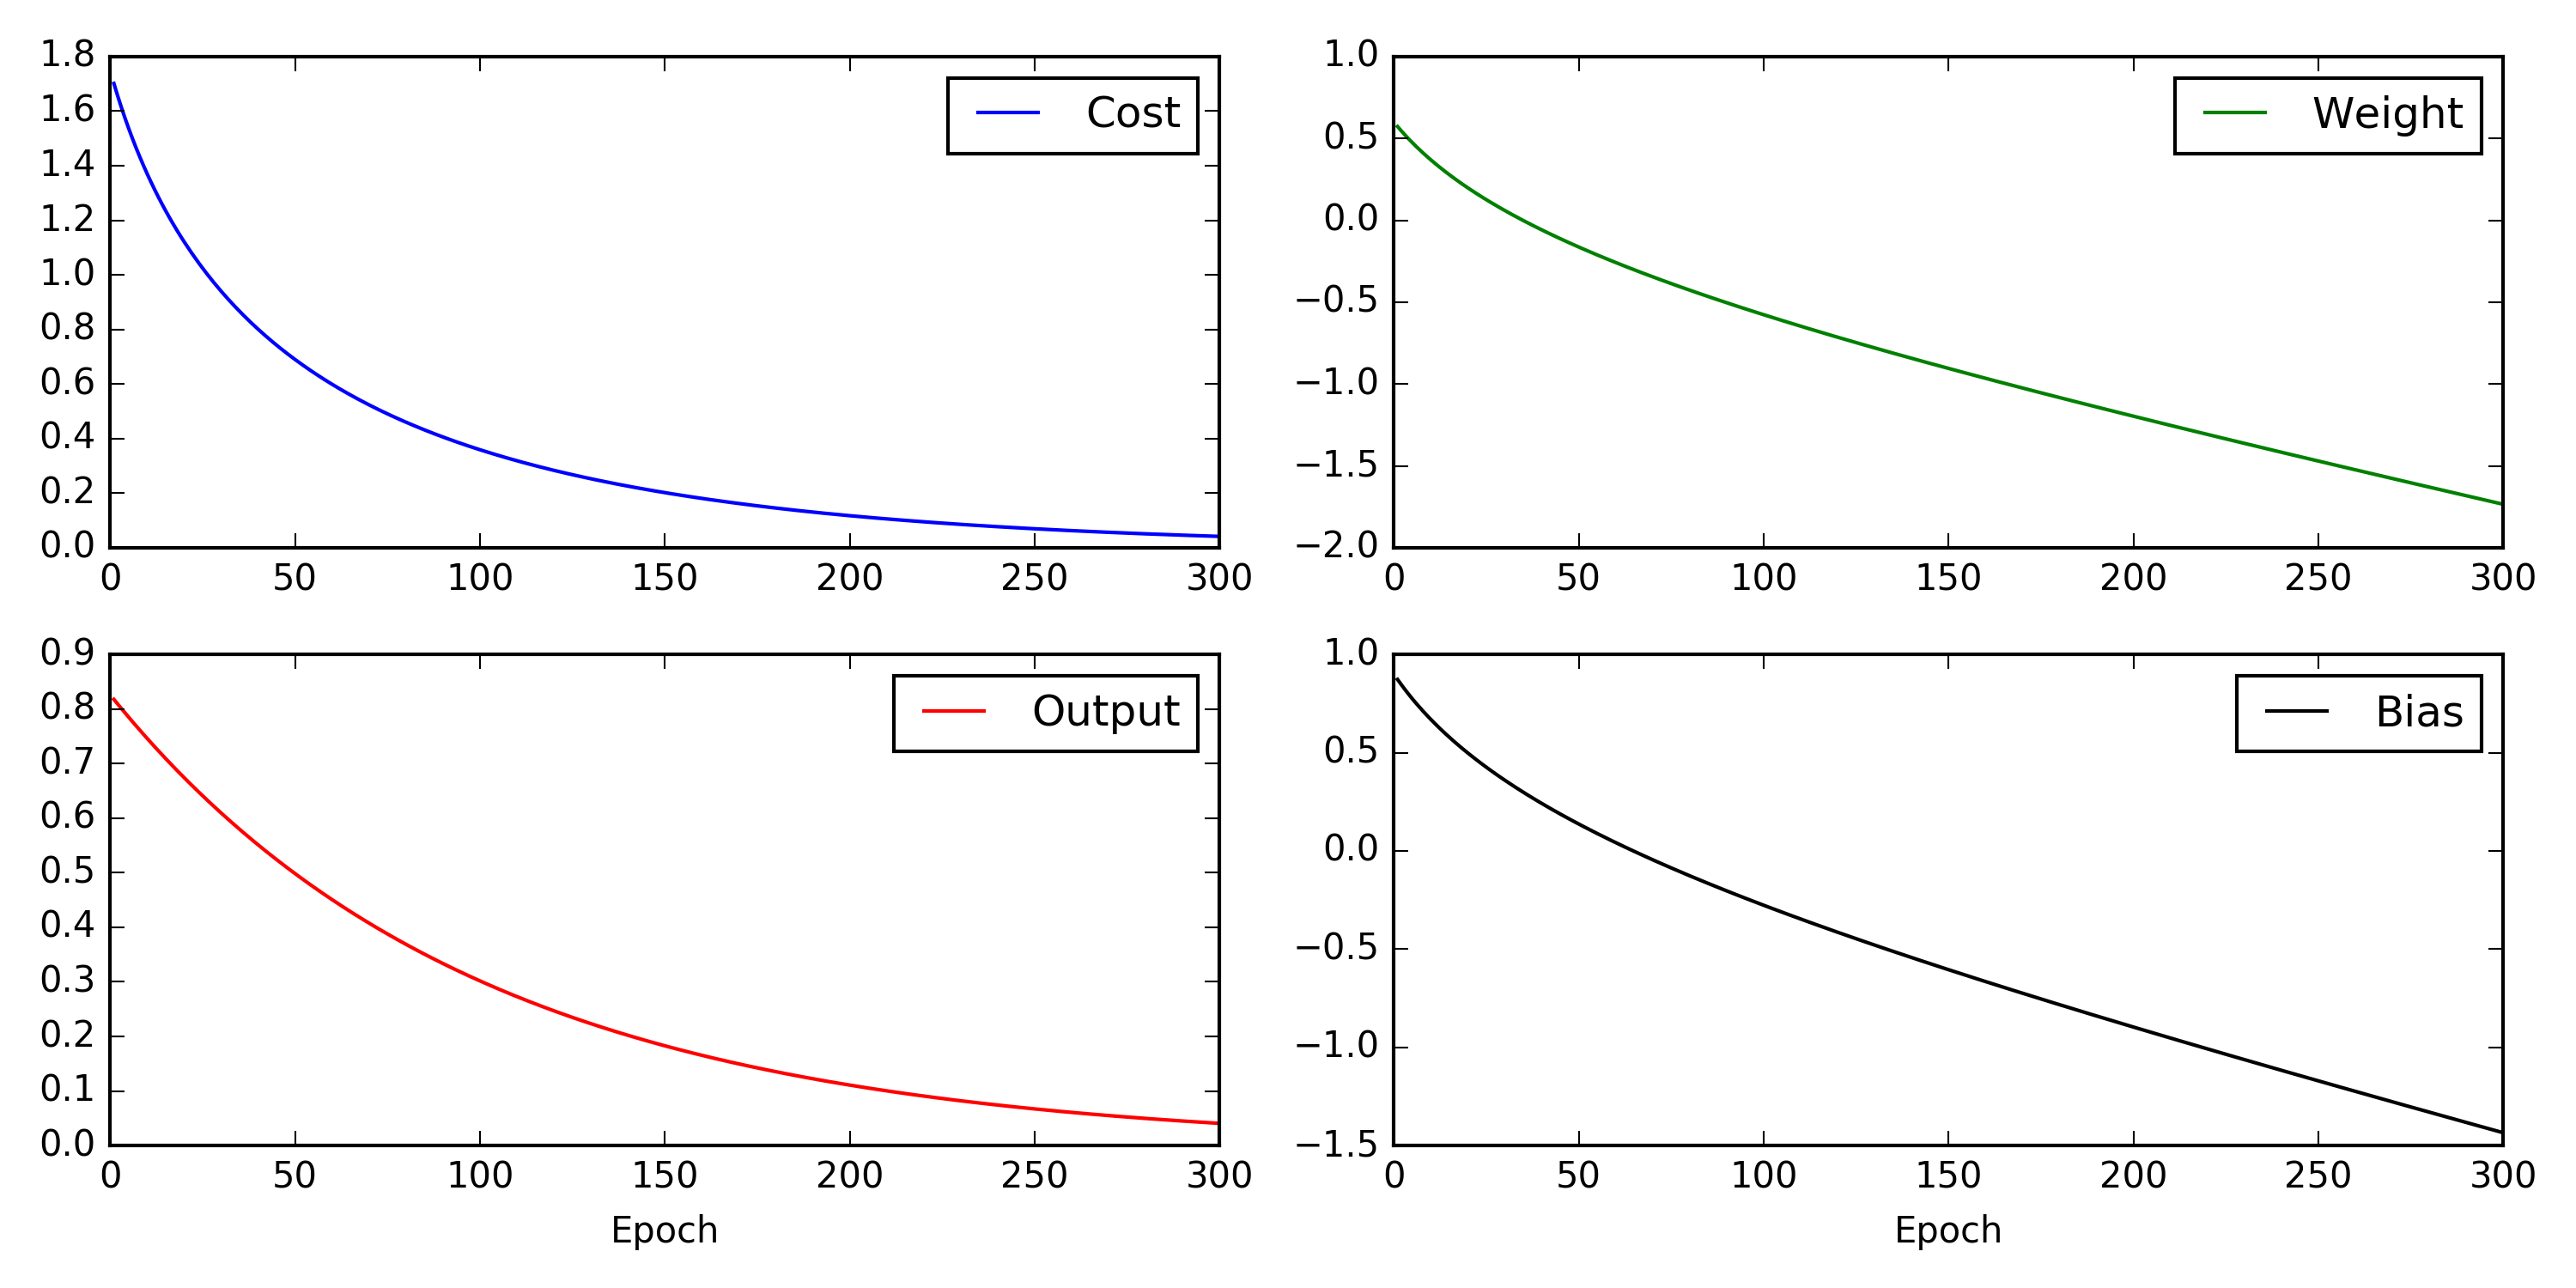
\includegraphics[width=0.8\linewidth]{./figures/ch3/animation_33}
\end{center}
Unsurprisingly, the neuron learns perfectly well in this instance, just as it did earlier. And now let's look at the case where our neuron got stuck before, with the weight and bias both starting at 2.0:
\begin{center}%
	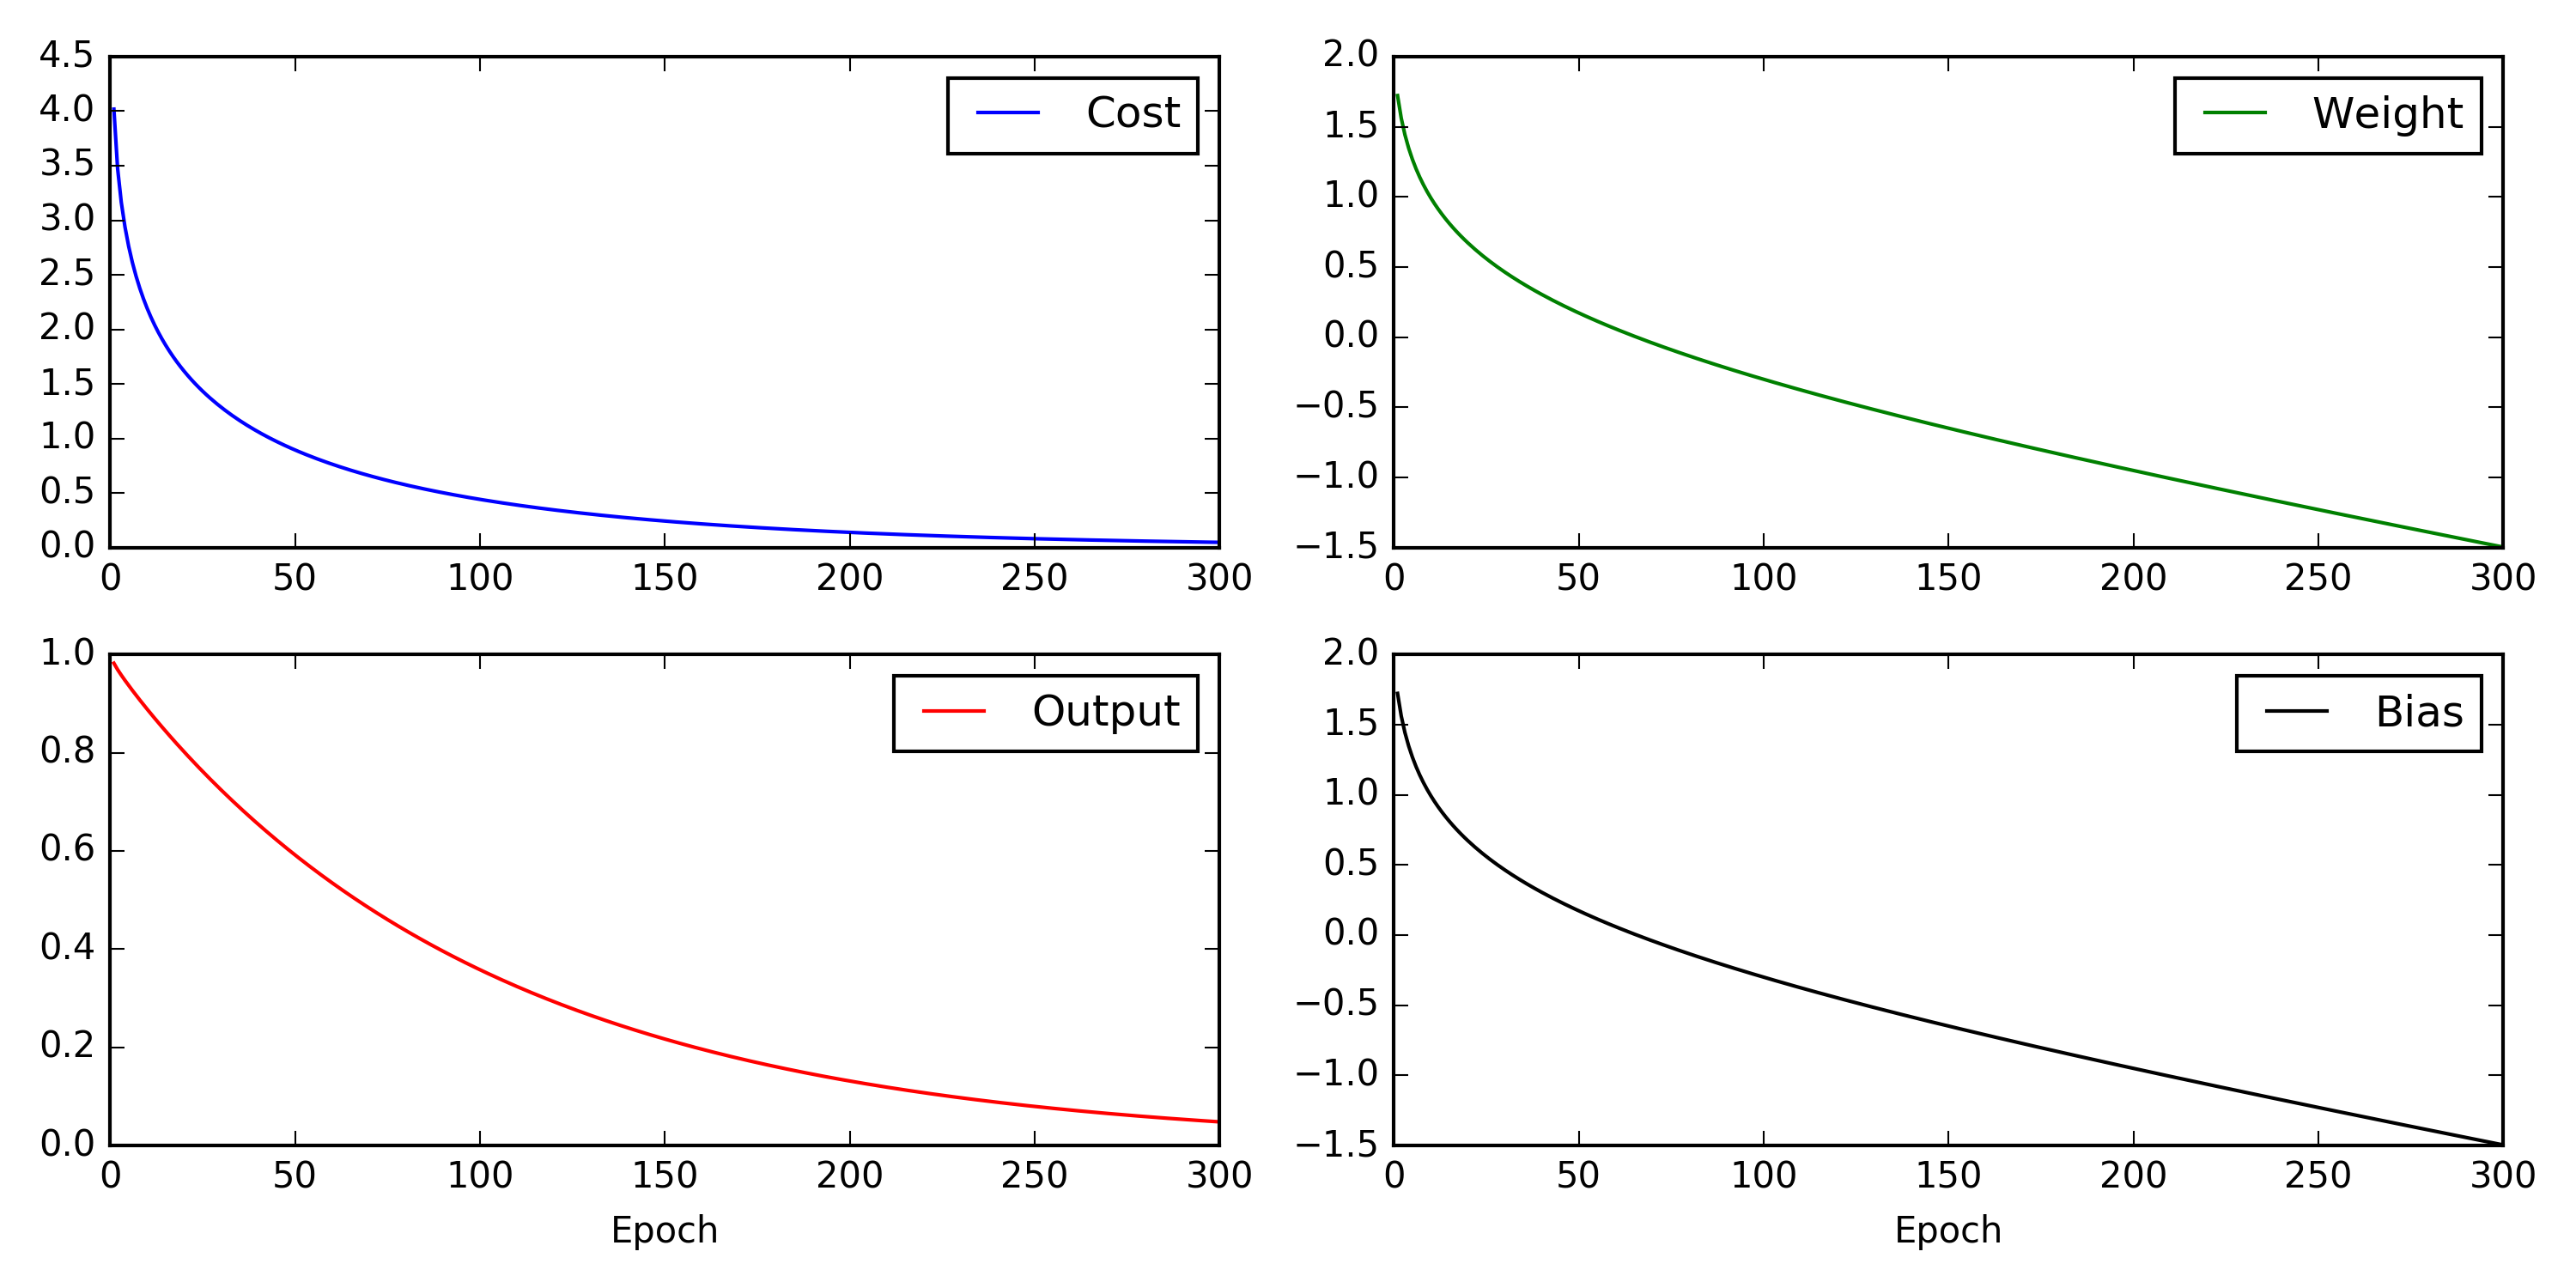
\includegraphics[width=0.8\linewidth]{./figures/ch3/animation_34}
\end{center}
Success! This time the neuron learned quickly, just as we hoped. If you observe closely you can see that the slope of the cost curve was much steeper initially than the initial flat region on the corresponding curve for the quadratic cost. It's that steepness which the cross-entropy buys us, preventing us from getting stuck just when we'd expect our neuron to learn fastest, i.e., when the neuron starts out badly wrong.

I didn't say what learning rate was used in the examples just illustrated. Earlier, with the quadratic cost, we used $\eta=0.15$. Should we have used the same learning rate in the new examples? In fact, with the change in cost function it's not possible to say precisely what it means to use the ``same'' learning rate; it's an apples and oranges comparison. For both cost functions I simply experimented to find a learning rate that made it possible to see what is going on. If you're still curious, despite my disavowal, here's the lowdown: I used $\eta=0.005$ in the examples just given.

You might object that the change in learning rate makes the graphs above meaningless. Who cares how fast the neuron learns, when our choice of learning rate was arbitrary to begin with?! That objection misses the point. The point of the graphs isn't about the absolute speed of learning. It's about how the speed of learning changes. In particular, when we use the quadratic cost learning is slower when the neuron is unambiguously wrong than it is later on, as the neuron gets closer to the correct output; while with the cross-entropy learning is faster when the neuron is unambiguously wrong. Those statements don't depend on how the learning rate is set.

We've been studying the cross-entropy for a single neuron. However, it's easy to generalize the cross-entropy to many-neuron multi-layer networks. In particular, suppose $y=y_1,y_2,\ldots$ are the desired values at the output neurons, i.e., the neurons in the final layer, while $a^L_1,a^L_2,\ldots$ are the actual output values. Then we define the cross-entropy by
%C=-1n∑x∑j[yjlna^L_j+(1-yj)ln(1-a^L_j)].(63)
\begin{equation}
	\sum_j \left[y_j \ln a^L_j + (1-y_j) \ln (1-a^L_j) \right].
	\label{eq:63}
\end{equation}
This is the same as our earlier expression, Equation (\ref{eq:57}), except now we've got the $\sum_j$ summing over all the output neurons. I won't explicitly work through a derivation, but it should be plausible that using the expression (\ref{eq:63}) avoids a learning slowdown in many-neuron networks. If you're interested, you can work through the derivation in the problem below.

Incidentally, I'm using the term ``cross-entropy'' in a way that has confused some early readers, since it superficially appears to conflict with other sources. In particular, it's common to define the cross-entropy for two probability distributions, $p_j$ and $q_j$, as $\sum_jp_j\ln{}q_j$. This definition may be connected to (\ref{eq:57}), if we treat a single sigmoid neuron as outputting a probability distribution consisting of the neuron's activation $a$ and its complement $1-a$.

However, when we have many sigmoid neurons in the final layer, the vector $a^L_j$ of activations don't usually form a probability distribution. As a result, a definition like $\sum_j p_j \ln q_j$ doesn't even make sense, since we're not working with probability distributions. Instead, you can think of (\ref{eq:63}) as a summed set of per-neuron cross-entropies, with the activation of each neuron being interpreted as part of a two-element probability distribution\footnote{Of course, in our networks there are no probabilistic elements, so they're not really probabilities.}. In this sense, (\ref{eq:63}) is a generalization of the cross-entropy for probability distributions.

When should we use the cross-entropy instead of the quadratic cost? In fact, the cross-entropy is nearly always the better choice, provided the output neurons are sigmoid neurons. To see why, consider that when we're setting up the network we usually initialize the weights and biases using some sort of randomization. It may happen that those initial choices result in the network being decisively wrong for some training input -- that is, an output neuron will have saturated near 1, when it should be 0, or vice versa. If we're using the quadratic cost that will slow down learning. It won't stop learning completely, since the weights will continue learning from other training inputs, but it's obviously undesirable.


\begin{exercize}{Exercises}
	\item One gotcha with the cross-entropy is that it can be difficult at first to remember the respective roles of the ys and the as. It's easy to get confused about whether the right form is $$-[y \ln a + (1-y) \ln (1-a)].$$ What happens to the second of these expressions when $y=0$ or 1? Does this problem afflict the first expression? Why or why not?
	\item In the single-neuron discussion at the start of this section, I argued that the cross-entropy is small if $\sigma(z)\approx y$ for all training inputs. The argument relied on $y$ being equal to either 0 or 1. This is usually true in classification problems, but for other problems (e.g., regression problems) $y$ can sometimes take values intermediate between 0 and 1. Show that the cross-entropy is still minimized when $\sigma(z)=y$ for all training inputs. When this is the case the cross-entropy has the value:
	\begin{equation}
		C = -\frac{1}{n} \sum_x [y \ln y+(1-y) \ln(1-y)].
		\label{eq:64}
	\end{equation}
	The quantity $-\left[y \ln y+(1-y) \ln(1-y)\right]$ is sometimes known as the \textit{binary entropy}.
\end{exercize}

\begin{exercize}{Problems}
	\item \textbf{Many-layer multi-neuron networks} In the notation introduced in the last chapter, show that for the quadratic cost the partial derivative with respect to weights in the output layer is
	\begin{equation}
		\frac{\partial C}{\partial w^L_{jk}}  = \frac{1}{n}
		\sum_x a^{L-1}_k  (a^L_j-y_j) \sigma'(z^L_j).
		\label{eq:65}
	\end{equation}%\partial{}C\partial{}w^L_{jk}=1n∑xaL-1k(a^L_j-yj)\sigma'(z^L_j).(65)
	The term $\sigma'(z^L_j)$ causes a learning slowdown whenever an output neuron saturates on the wrong value. Show that for the cross-entropy cost the output error 
	$\delta^L$ for a single training example $x$ is given by
	\begin{equation}
		\delta^L = a^L - y.\label{eq:66}
	\end{equation}%δL=aL-y.(66)
	Use this expression to show that the partial derivative with respect to the weights in the output layer is given by
	\begin{equation}
		\frac{\partial C}{\partial w^L_{jk}}  =  \frac{1}{n} \sum_x 	a^{L-1}_k  (a^L_j-y_j).
		\label{eq:67}
	\end{equation}%\partial{}C\partial{}w^L_{jk}=1n∑xaL-1k(a^L_j-yj).(67)
	The $\sigma'(z^L_j)$ term has vanished, and so the cross-entropy avoids the problem of learning slowdown, not just when used with a single neuron, as we saw earlier, but also in many-layer multi-neuron networks. A simple variation on this analysis holds also for the biases. If this is not obvious to you, then you should work through that analysis as well.
	\item \textbf{Using the quadratic cost when we have linear neurons in the output layer} Suppose that we have a many-layer multi-neuron network. Suppose all the neurons in the final layer are linear neurons, meaning that the sigmoid activation function is not applied, and the outputs are simply $a^L_j=z^L_j$. Show that if we use the quadratic cost function then the output error $\delta^L$ for a single training example $x$ is given by
	\begin{equation}
		\delta^L = a^L-y.
		\label{eq:68}
	\end{equation}%δL=aL-y.(68)
	Similarly to the previous problem, use this expression to show that the partial derivatives with respect to the weights and biases in the output layer are given by
	\begin{align}
	\frac{\partial C}{\partial w^L_{jk}} &=  \frac{1}{n} \sum_x a^{L-1}_k  (a^L_j-y_j)\label{eq:69}\\
	\frac{\partial C}{\partial b^L_{j}} &=  \frac{1}{n} \sum_x (a^L_j-y_j).
	\label{eq:70}
	\end{align}
	%\partial{}C\partial{}w^L_{jk}\partial{}C\partial{}b^L_j==1n∑xaL-1k(a^L_j-yj)1n∑x(a^L_j-yj).(69)(70)
	This shows that if the output neurons are linear neurons then the quadratic cost will not give rise to any problems with a learning slowdown. In this case the quadratic cost is, in fact, an appropriate cost function to use.
\end{exercize}
\subsection{Using the cross-entropy to classify MNIST digits}
The cross-entropy is easy to implement as part of a program which learns using gradient descent and backpropagation. We'll do that later in the chapter, developing an improved version of our earlier program for classifying the MNIST handwritten digits, \inline{network.py}. The new program is called \inline{network2.py}, and incorporates not just the cross-entropy, but also several other techniques developed in this chapter\footnote{The code is available on \href{https://github.com/mnielsen/neural-networks-and-deep-learning/blob/master/src/network2.py}{GitHub}.}. For now, let's look at how well our new program classifies MNIST digits. As was the case in Chapter 1, we'll use a network with 30 hidden neurons, and we'll use a mini-batch size of 10. We set the learning rate to $\eta=0.5$\footnote{In Chapter 1 we used the quadratic cost and a learning rate of $\eta=3.0$. As discussed above, it's not possible to say precisely what it means to use the ``same'' learning rate when the cost function is changed. For both cost functions I experimented to find a learning rate that provides near-optimal performance, given the other hyper-parameter choices. \newline There is, incidentally, a very rough general heuristic for relating the learning rate for the cross-entropy and the quadratic cost. As we saw earlier, the gradient terms for the quadratic cost have an extra $\sigma' = \sigma(1-\sigma)$ term in them. Suppose we average this over values for $\sigma$, $\int_0^1\mathrm{d}\sigma \sigma(1-\sigma)=1/6$. We see that (very roughly) the quadratic cost learns an average of 6 times slower, for the same learning rate. This suggests that a reasonable starting point is to divide the learning rate for the quadratic cost by 6. Of course, this argument is far from rigorous, and shouldn't be taken too seriously. Still, it can sometimes be a useful starting point.} and we train for 30 epochs. The interface to \inline{network2.py} is slightly different than \inline{network.py}, but it should still be clear what is going on. You can, by the way, get documentation about \inline{network2.py}'s interface by using commands such as \inline{help(network2.Network.SGD)} in a Python shell.
\begin{lstlisting}
>>> import mnist_loader
>>> training_data, validation_data, test_data = mnist_loader.load_data_wrapper()
>>> import network2
>>> net = network2.Network([784, 30, 10], cost=network2.CrossEntropyCost)
>>> net.large_weight_initializer()
>>> net.SGD(training_data, 30, 10, 0.5, evaluation_data=test_data, monitor_evaluation_accuracy=True)
\end{lstlisting}	
Note, by the way, that the \inline{net.large_weight_initializer()} command is used to initialize the weights and biases in the same way as described in Chapter 1. We need to run this command because later in this chapter we'll change the default weight initialization in our networks. The result from running the above sequence of commands is a network with 95.49 percent accuracy. This is pretty close to the result we obtained in Chapter 1, 95.42 percent, using the quadratic cost.
	
Let's look also at the case where we use 100 hidden neurons, the cross-entropy, and otherwise keep the parameters the same. In this case we obtain an accuracy of 96.82 percent. That's a substantial improvement over the results from Chapter 1, where we obtained a classification accuracy of 96.59 percent, using the quadratic cost. That may look like a small change, but consider that the error rate has dropped from 3.41 percent to 3.18 percent. That is, we've eliminated about one in fourteen of the original errors. That's quite a handy improvement.
	
It's encouraging that the cross-entropy cost gives us similar or better results than the quadratic cost. However, these results don't conclusively prove that the cross-entropy is a better choice. The reason is that I've put only a little effort into choosing hyper-parameters such as learning rate, mini-batch size, and so on. For the improvement to be really convincing we'd need to do a thorough job optimizing such hyper-parameters. Still, the results are encouraging, and reinforce our earlier theoretical argument that the cross-entropy is a better choice than the quadratic cost.
	
This, by the way, is part of a general pattern that we'll see through this chapter and, indeed, through much of the rest of the book. We'll develop a new technique, we'll try it out, and we'll get ``improved'' results. It is, of course, nice that we see such improvements. But the interpretation of such improvements is always problematic. They're only truly convincing if we see an improvement after putting tremendous effort into optimizing all the other hyper-parameters. That's a great deal of work, requiring lots of computing power, and we're not usually going to do such an exhaustive investigation. Instead, we'll proceed on the basis of informal tests like those done above. Still, you should keep in mind that such tests fall short of definitive proof, and remain alert to signs that the arguments are breaking down.
	
By now, we've discussed the cross-entropy at great length. Why go to so much effort when it gives only a small improvement to our MNIST results? Later in the chapter we'll see other techniques -- notably, regularization -- which give much bigger improvements. So why so much focus on cross-entropy? Part of the reason is that the cross-entropy is a widely-used cost function, and so is worth understanding well. But the more important reason is that neuron saturation is an important problem in neural nets, a problem we'll return to repeatedly throughout the book. And so I've discussed the cross-entropy at length because it's a good laboratory to begin understanding neuron saturation and how it may be addressed.

\subsection{What does the cross-entropy mean? Where does it come from?}
Our discussion of the cross-entropy has focused on algebraic analysis and practical implementation. That's useful, but it leaves unanswered broader conceptual questions, like: what does the cross-entropy mean? Is there some intuitive way of thinking about the cross-entropy? And how could we have dreamed up the cross-entropy in the first place?

Let's begin with the last of these questions: what could have motivated us to think up the cross-entropy in the first place? Suppose we'd discovered the learning slowdown described earlier, and understood that the origin was the $\sigma'(z)$ terms in Equations (\ref{eq:55}) and (\ref{eq:56}). After staring at those equations for a bit, we might wonder if it's possible to choose a cost function so that the $\sigma'(z)$ term disappeared. In that case, the cost $C=C_x$ for a single training example $x$ would satisfy
\begin{eqnarray} 
\frac{\partial C}{\partial w_j} & = & x_j(a-y) \label{eq:71}\\
\frac{\partial C}{\partial b } & = & (a-y).
\label{eq:72}\end{eqnarray}
%\partial{}C\partial{}wj\partial{}C\partial{}b==x_j(a-y)(a-y).(71)(72)
If we could choose the cost function to make these equations true, then they would capture in a simple way the intuition that the greater the initial error, the faster the neuron learns. They'd also eliminate the problem of a learning slowdown. In fact, starting from these equations we'll now show that it's possible to derive the form of the cross-entropy, simply by following our mathematical noses. To see this, note that from the chain rule we have
\begin{equation}
	\frac{\partial C}{\partial b} = \frac{\partial C}{\partial a} \sigma'(z).
	\label{eq:73}
\end{equation}
%\partial{}C\partial{}b=\partial{}C\partial{}a\sigma'(z).(73)
Using $\sigma'(z)=\sigma(z)(1-\sigma(z))=a(1-a)$ the last equation becomes
\begin{eqnarray}
\frac{\partial C}{\partial b} = \frac{\partial C}{\partial a} 
a(1-a).
\label{eq:74}\end{eqnarray}
%\partial{}C\partial{}b=\partial{}C\partial{}aa(1-a).(74)
Comparing to Equation~\ref{eq:72} we obtain
\begin{eqnarray}
\frac{\partial C}{\partial a} = \frac{a-y}{a(1-a)}. \label{eq:75}\end{eqnarray}
Integrating this expression with respect to $a$ gives
\begin{eqnarray}
C = -[y \ln a + (1-y) \ln (1-a)]+ {\rm constant},
\label{eq:76}\end{eqnarray}
%C=-[ylna+(1-y)ln(1-a)]+constant,(76)
for some constant of integration. This is the contribution to the cost from a single training example, $x$. To get the full cost function we must average over training examples, obtaining
\begin{eqnarray}
C = -\frac{1}{n} \sum_x [y \ln a +(1-y) \ln(1-a)] + {\rm constant},
\label{eq:77}\end{eqnarray}
where the constant here is the average of the individual constants for each training example. And so we see that Equations (\ref{eq:71}) and (\ref{eq:72}) uniquely determine the form of the cross-entropy, up to an overall constant term. The cross-entropy isn't something that was miraculously pulled out of thin air. Rather, it's something that we could have discovered in a simple and natural way.

What about the intuitive meaning of the cross-entropy? How should we think about it? Explaining this in depth would take us further afield than I want to go. However, it is worth mentioning that there is a standard way of interpreting the cross-entropy that comes from the field of information theory. Roughly speaking, the idea is that the cross-entropy is a measure of surprise. In particular, our neuron is trying to compute the function $x\to y=y(x)$. But instead it computes the function $x \to a=a(x)$. Suppose we think of a as our neuron's estimated probability that $y$ is 1, and $1-a$ is the estimated probability that the right value for $y$ is 0. Then the cross-entropy measures how ``surprised'' we are, on average, when we learn the true value for $y$. We get low surprise if the output is what we expect, and high surprise if the output is unexpected. Of course, I haven't said exactly what ``surprise'' means, and so this perhaps seems like empty verbiage. But in fact there is a precise information-theoretic way of saying what is meant by surprise. Unfortunately, I don't know of a good, short, self-contained discussion of this subject that's available online. But if you want to dig deeper, then Wikipedia contains a \href{http://en.wikipedia.org/wiki/Cross_entropy#Motivation}{brief summary} that will get you started down the right track. And the details can be filled in by working through the materials about the Kraft inequality in chapter 5 of the book about information theory by \href{http://books.google.ca/books?id=VWq5GG6ycxMC}{Cover and Thomas}.


\begin{exercize}{Problem}
	\item We've discussed at length the learning slowdown that can occur when output neurons saturate, in networks using the quadratic cost to train. Another factor that may inhibit learning is the presence of the $x_j$ term in Equation (\ref{eq:61}). Because of this term, when an input $x_j$ is near to zero, the corresponding weight $w_j$ will learn slowly. Explain why it is not possible to eliminate the $x_j$ term through a clever choice of cost function.
\end{exercize}

\subsection{Softmax}
In this chapter we'll mostly use the cross-entropy cost to address the problem of learning slowdown. However, I want to briefly describe another approach to the problem, based on what are called \textit{softmax} layers of neurons. We're not actually going to use softmax layers in the remainder of the chapter, so if you're in a great hurry, you can skip to the next section. However, softmax is still worth understanding, in part because it's intrinsically interesting, and in part because we'll use softmax layers in Chapter 6, in our discussion of deep neural networks.

The idea of softmax is to define a new type of output layer for our neural networks. It begins in the same way as with a sigmoid layer, by forming the weighted inputs\footnote{In describing the softmax we'll make frequent use of notation introduced in the last chapter. You may wish to revisit that chapter if you need to refresh your memory about the meaning of the notation.} $z^L_j=\sum_kw^L_{jk}a^{L-1}_k+b^L_j$. However, we don't apply the sigmoid function to get the output. Instead, in a softmax layer we apply the so-called softmax function to the $z^L_j$. According to this function, the activation $a^L_j$ of the $j$-th output neuron is
\begin{equation}
	a^L_j = \frac{e^{x^L_j}}{\sum_ke^{z^L_k}}
	\label{eq:78}
\end{equation}
%a^L_j=ez^L_j∑kezLk,(78)
where in the denominator we sum over all the output neurons.

If you're not familiar with the softmax function, Equation (\ref{eq:78}) may look pretty opaque. It's certainly not obvious why we'd want to use this function. And it's also not obvious that this will help us address the learning slowdown problem. To better understand Equation (\ref{eq:78}), suppose we have a network with four output neurons, and four corresponding weighted inputs, which we'll denote $z^L_1,z^L_2,z^L_3,$ and $z^L_4$. Figure~\ref{fig:softmax} shows  a graph of the corresponding output activations for different inputs\footnote{This paragraph is an adaptation of an animation from online version of the book.}.
%\begin{center}
%\begin{tikzpicture}
%\begin{axis}[xmin=-5,xmax=5,ymin=0,ymax=1,xlabel={$z_4$},ylabel={$a_j$},width=0.9\linewidth,height=0.4\linewidth,legend cell align={left}]
%	\addplot[domain=-5:5,samples=101,blue!75] {exp(-1)/(exp(x)+exp(1)+exp(0)+exp(-1))};
%	\addplot[domain=-5:5,samples=101,orange!75] {exp(0)/(exp(x)+exp(1)+exp(0)+exp(-1))};
%	\addplot[domain=-5:5,samples=101,green!75!black] {exp(1)/(exp(x)+exp(1)+exp(0)+exp(-1))};
%	\addplot[domain=-5:5,samples=101,red!75] {exp(x)/(exp(x)+exp(1)+exp(0)+exp(-1))};
%	\addlegendentry{$a_1,z_1=-1$};
%	\addlegendentry{$a_2,z_2=0$};
%	\addlegendentry{$a_3,z_3=1$};
%	\addlegendentry{$a_4$};	
%\end{axis}
%\end{tikzpicture}
%%\begin{tikzpicture}
%%\begin{axis}[xmin=-5,xmax=5,ymin=0,ymax=1,xlabel={$z_4$},ylabel={$a_j$},width=0.49\linewidth,height=0.35\linewidth,legend cell align={left}]
%%	\addplot[domain=-5:5,samples=101,blue!75] {exp(-0.5)/(exp(x)+exp(1.5)+exp(0.5)+exp(-1.5))};
%%	\addplot[domain=-5:5,samples=101,orange!75] {exp(0.5)/(exp(x)+exp(1.5)+exp(0.5)+exp(-1.5))};
%%	\addplot[domain=-5:5,samples=101,green!75!black] {exp(1.5)/(exp(x)+exp(1.5)+exp(0.5)+exp(-1.5))};
%%	\addplot[domain=-5:5,samples=101,red!75] {exp(x)/(exp(x)+exp(1.5)+exp(0.5)+exp(-1.5))};
%%	\addlegendentry{$a_1,z_1=-0.5$};
%%	\addlegendentry{$a_2,z_2=0.5$};
%%	\addlegendentry{$a_3,z_3=1.5$};
%%	\addlegendentry{$a_4$};	
%%\end{axis}
%%\end{tikzpicture}
%\end{center}
\begin{figure}
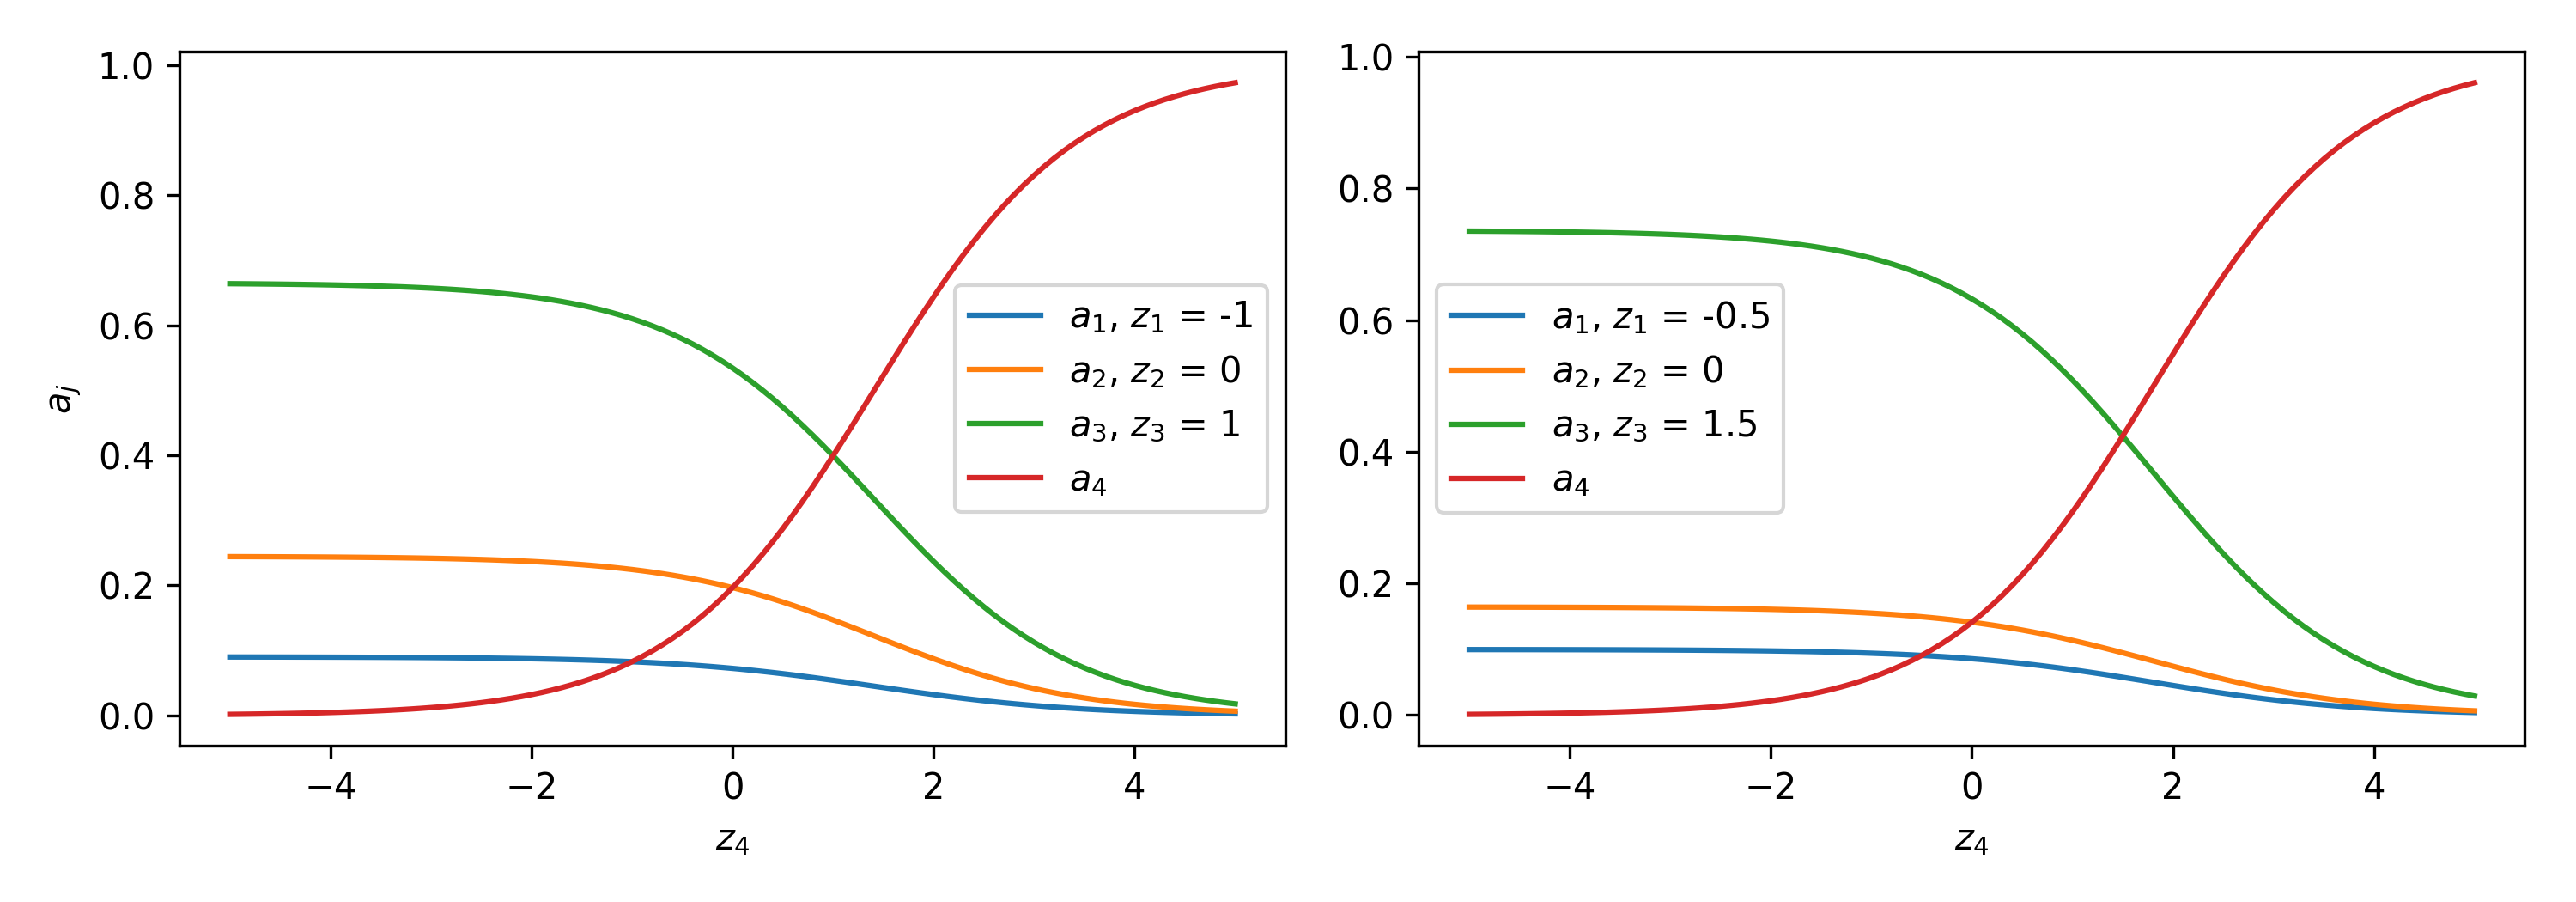
\includegraphics[width=\linewidth]{./figures/ch3/animation_softmax}
\caption{Equation~\ref{eq:78} for different fixed values of $z^L_{1,2,3}$ and variable $z^L_4$. $L$ index avoided for clarity. }
\label{fig:softmax}
\end{figure}
As you increase $z^L_4$, you'll see an increase in the corresponding output activation, $a^L_4$, and a decrease in the other output activations. Similarly, if you decrease $z^L_4$ then $a^L_4$ will decrease, and all the other output activations will increase. In fact, if you look closely, you'll see that in both cases the total change in the other activations exactly compensates for the change in $a^L_4$. The reason is that the output activations are guaranteed to always sum up to 1, as we can prove using Equation (\ref{eq:78}) and a little algebra:
\begin{eqnarray}
\sum_j a^L_j & = & \frac{\sum_j e^{z^L_j}}{\sum_k e^{z^L_k}} = 1.
\label{eq:79}\end{eqnarray}
%∑ja^L_j=∑jez^L_j∑kezLk=1.(79)
As a result, if $a^L_4$ increases, then the other output activations must decrease by the same total amount, to ensure the sum over all activations remains 1. And, of course, similar statements hold for all the other activations.

Equation (\ref{eq:78}) also implies that the output activations are all positive, since the exponential function is positive. Combining this with the observation in the last paragraph, we see that the output from the softmax layer is a set of positive numbers which sum up to 1. In other words, the output from the softmax layer can be thought of as a probability distribution.

The fact that a softmax layer outputs a probability distribution is rather pleasing. In many problems it's convenient to be able to interpret the output activation $a^L_j$ as the network's estimate of the probability that the correct output is $j$. So, for instance, in the MNIST classification problem, we can interpret $a^L_j$ as the network's estimated probability that the correct digit classification is $j$.

By contrast, if the output layer was a sigmoid layer, then we certainly couldn't assume that the activations formed a probability distribution. I won't explicitly prove it, but it should be plausible that the activations from a sigmoid layer won't in general form a probability distribution. And so with a sigmoid output layer we don't have such a simple interpretation of the output activations.

\begin{exercize}{Exercise}
	\item Construct an example showing explicitly that in a network with a sigmoid output layer, the output activations $a^L_j$ won't always sum to 1.
\end{exercize}
We're starting to build up some feel for the softmax function and the way softmax layers behave. Just to review where we're at: the exponentials in Equation (\ref{eq:78}) ensure that all the output activations are positive. And the sum in the denominator of Equation (\ref{eq:78}) ensures that the softmax outputs sum to 1. So that particular form no longer appears so mysterious: rather, it is a natural way to ensure that the output activations form a probability distribution. You can think of softmax as a way of rescaling the $z^L_j$, and then squishing them together to form a probability distribution.


\begin{exercize}{Exercises}
\item \textbf{Monotonicity of softmax} Show that $\partial a^L_j / \partial z^L_k $ is positive if $j=k$ and negative if $j\ne k$. As a consequence, increasing $z^L_j$ is guaranteed to increase the corresponding output activation, $a^L_j$, and will decrease all the other output activations. We already saw this empirically with the sliders, but this is a rigorous proof.
\item \textbf{Non-locality of softmax} A nice thing about sigmoid layers is that the output $a^L_j$ is a function of the corresponding weighted input, $a^L_j=\sigma(z^L_j)$. Explain why this is not the case for a softmax layer: any particular output activation $a^L_j$ depends on all the weighted inputs.
\end{exercize}

\begin{exercize}{Problem}
	\item \textbf{Inverting the softmax layer} Suppose we have a neural network with a softmax output layer, and the activations $a^L_j$ are known. Show that the corresponding weighted inputs have the form $z^L_j=\ln a^L_j+C$, for some constant $C$ that is independent of $j$.
\end{exercize}
\textbf{The learning slowdown problem:} We've now built up considerable familiarity with softmax layers of neurons. But we haven't yet seen how a softmax layer lets us address the learning slowdown problem. To understand that, let's define the \textit{log-likelihood} cost function. We'll use $x$ to denote a training input to the network, and $y$ to denote the corresponding desired output. Then the log-likelihood cost associated to this training input is
%C≡-lnaLy.(80)
\begin{equation}
	C \equiv -\ln a^L_j
\label{eq:80}
\end{equation}
So, for instance, if we're training with MNIST images, and input an image of a 7, then the log-likelihood cost is $-\ln a^L_7$. To see that this makes intuitive sense, consider the case when the network is doing a good job, that is, it is confident the input is a 7. In that case it will estimate a value for the corresponding probability $a^L_7$ which is close to 1, and so the cost $-\ln a^L_7$ will be small. By contrast, when the network isn't doing such a good job, the probability $a^L_7$ will be smaller, and the cost $-\ln a^L_7$ will be larger. So the log-likelihood cost behaves as we'd expect a cost function to behave.

What about the learning slowdown problem? To analyze that, recall that the key to the learning slowdown is the behaviour of the quantities $\partial C/\partial w^L_{jk}$ and $\partial C/\partial b^L_j$. I won't go through the derivation explicitly -- I'll ask you to do in the problems, below -- but with a little algebra you can show that\footnote{Note that I'm abusing notation here, using $y$ in a slightly different way to last paragraph. In the last paragraph we used $y$ to denote the desired output from the network -- e.g., output a ``7'' if an image of a 7 was input. But in the equations which follow I'm using $y$ to denote the vector of output activations which corresponds to 7, that is, a vector which is all 0s, except for a 1 in the 7th location.}
%\partial C\partial b^L_j\partial C\partial w^L_{jk}==a^L_j-yjaL-1k(a^L_j-yj)(81)(82)
\begin{eqnarray}
\frac{\partial C}{\partial b^L_j} & = & a^L_j-y_j  \label{eq:81}\\
\frac{\partial C}{\partial w^L_{jk}} & = & a^{L-1}_k (a^L_j-y_j)\label{eq:82}
\end{eqnarray}
These equations are the same as the analogous expressions obtained in our earlier analysis of the cross-entropy. Compare, for example, Equation (\ref{eq:82}) to Equation (\ref{eq:67}). It's the same equation, albeit in the latter I've averaged over training instances. And, just as in the earlier analysis, these expressions ensure that we will not encounter a learning slowdown. In fact, it's useful to think of a softmax output layer with log-likelihood cost as being quite similar to a sigmoid output layer with cross-entropy cost.

Given this similarity, should you use a sigmoid output layer and cross-entropy, or a softmax output layer and log-likelihood? In fact, in many situations both approaches work well. Through the remainder of this chapter we'll use a sigmoid output layer, with the cross-entropy cost. Later, in Chapter 6, we'll sometimes use a softmax output layer, with log-likelihood cost. The reason for the switch is to make some of our later networks more similar to networks found in certain influential academic papers. As a more general point of principle, softmax plus log-likelihood is worth using whenever you want to interpret the output activations as probabilities. That's not always a concern, but can be useful with classification problems (like MNIST) involving disjoint classes.


\begin{exercize}{Problems}
\item Derive Equations (\ref{eq:81}) and (\ref{eq:82}).
\item \textbf{Where does the ``softmax'' name come from?} Suppose we change the softmax function so the output activations are given by
\begin{equation}
	a^L_j = \frac{e^{c z^L_j}}{\sum_k e^{c z^L_k}},\label{eq:83}
\end{equation}
where $c$ is a positive constant. Note that $c=1$ corresponds to the standard softmax function. But if we use a different value of $c$ we get a different function, which is nonetheless qualitatively rather similar to the softmax. In particular, show that the output activations form a probability distribution, just as for the usual softmax. Suppose we allow $c$ to become large, i.e., $c\to \infty$. What is the limiting value for the output activations $a^L_j$? After solving this problem it should be clear to you why we think of the $c=1$ function as a ``softened'' version of the maximum function. This is the origin of the term ``softmax''.
\item \textbf{Backpropagation with softmax and the log-likelihood cost} In the last chapter we derived the backpropagation algorithm for a network containing sigmoid layers. To apply the algorithm to a network with a softmax layer we need to figure out an expression for the error $\delta^L_j \equiv \partial C / \partial z^L_j$ in the final layer. Show that a suitable expression is:
\begin{equation}
\delta^L_j = a^L_j -y_j. \label{eq:84}
\end{equation}
Using this expression we can apply the backpropagation algorithm to a network using a softmax output layer and the log-likelihood cost.
\end{exercize}

\section{Overfitting and regularization}
\label{sec:3.2}
The Nobel prize winning physicist Enrico Fermi was once asked his opinion of a mathematical model some colleagues had proposed as the solution to an important unsolved physics problem. The model gave excellent agreement with experiment, but Fermi was skeptical. He asked how many free parameters could be set in the model. ``Four'' was the answer. Fermi replied\footnote{The quote comes from a charming article by \href{http://www.nature.com/nature/journal/v427/n6972/full/427297a.html}{Freeman Dyson}, who is one of the people who proposed the flawed model. A four-parameter elephant may be found \href{http://www.johndcook.com/blog/2011/06/21/how-to-fit-an-elephant/}{here}.} : ``I remember my friend Johnny von Neumann used to say, with four parameters I can fit an elephant, and with five I can make him wiggle his trunk.''.

The point, of course, is that models with a large number of free parameters can describe an amazingly wide range of phenomena. Even if such a model agrees well with the available data, that doesn't make it a good model. It may just mean there's enough freedom in the model that it can describe almost any data set of the given size, without capturing any genuine insights into the underlying phenomenon. When that happens the model will work well for the existing data, but will fail to generalize to new situations. The true test of a model is its ability to make predictions in situations it hasn't been exposed to before.

Fermi and von Neumann were suspicious of models with four parameters. Our 30 hidden neuron network for classifying MNIST digits has nearly 24,000 parameters! That's a lot of parameters. Our 100 hidden neuron network has nearly 80,000 parameters, and state-of-the-art deep neural nets sometimes contain millions or even billions of parameters. Should we trust the results?

Let's sharpen this problem up by constructing a situation where our network does a bad job generalizing to new situations. We'll use our 30 hidden neuron network, with its 23,860 parameters. But we won't train the network using all 50,000 MNIST training images. Instead, we'll use just the first 1,000 training images. Using that restricted set will make the problem with generalization much more evident. We'll train in a similar way to before, using the cross-entropy cost function, with a learning rate of $\eta=0.5$ and a mini-batch size of 10. However, we'll train for 400 epochs, a somewhat larger number than before, because we're not using as many training examples. Let's use \inline{network2} to look at the way the cost function changes:


\begin{lstlisting}

>>> import mnist_loader 
>>> training_data, validation_data, test_data = mnist_loader.load_data_wrapper()
>>> import network2 
>>> net = network2.Network([784, 30, 10], cost=network2.CrossEntropyCost) 
>>> net.large_weight_initializer()
>>> net.SGD(training_data[:1000], 400, 10, 0.5, evaluation_data=test_data, monitor_evaluation_accuracy=True, monitor_training_cost=True)
\end{lstlisting}
Using the results we can plot the way the cost changes as the network learns\footnote{This and the next four graphs were generated by the program \href{https://github.com/mnielsen/neural-networks-and-deep-learning/blob/master/fig/overfitting.py}{overfitting.py}.} :

\begin{center}
	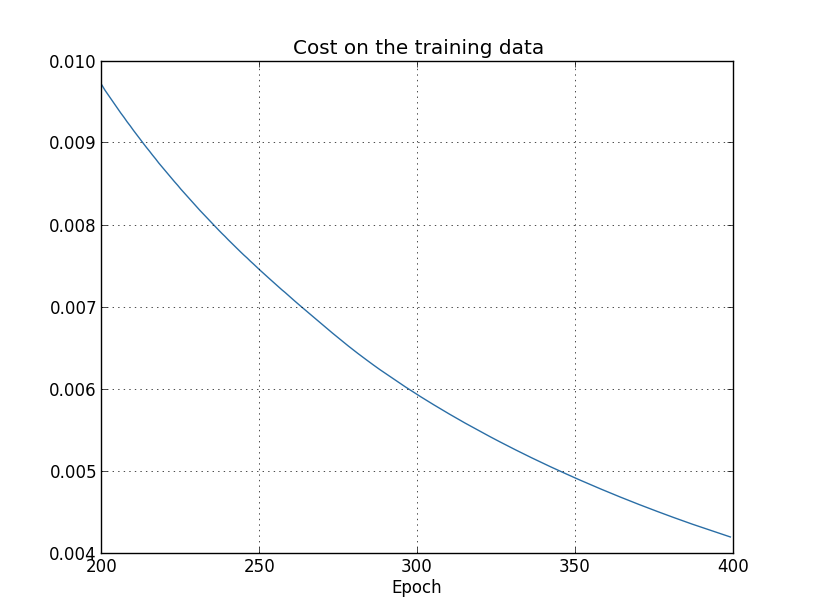
\includegraphics[width=0.6\linewidth]{figures/ch3/overfitting1}
\end{center}
This looks encouraging, showing a smooth decrease in the cost, just as we expect. Note that I've only shown training epochs 200 through 399. This gives us a nice up-close view of the later stages of learning, which, as we'll see, turns out to be where the interesting action is.

Let's now look at how the classification accuracy on the test data changes over time:
\begin{center}
	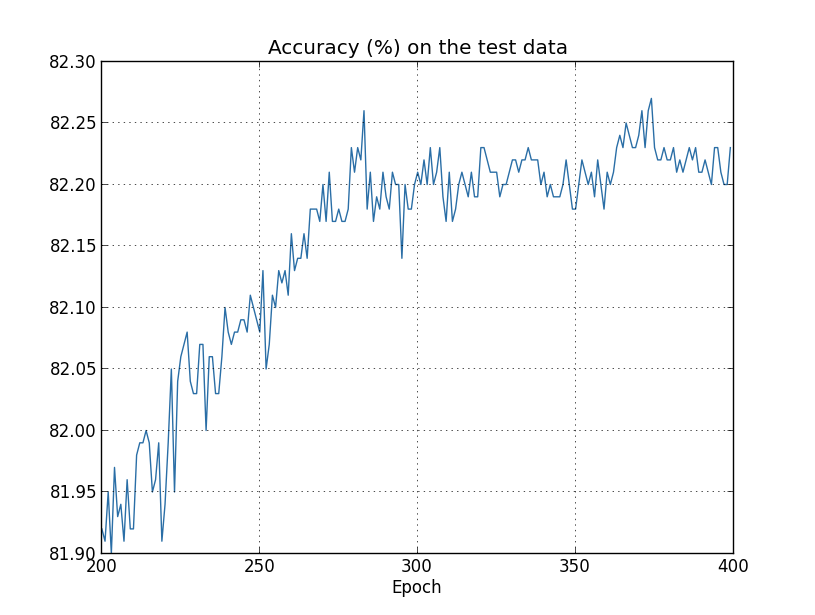
\includegraphics[width=0.6\linewidth]{figures/ch3/overfitting2}
\end{center}
Again, I've zoomed in quite a bit. In the first 200 epochs (not shown) the accuracy rises to just under 82 percent. The learning then gradually slows down. Finally, at around epoch 280 the classification accuracy pretty much stops improving. Later epochs merely see small stochastic fluctuations near the value of the accuracy at epoch 280. Contrast this with the earlier graph, where the cost associated to the training data continues to smoothly drop. If we just look at that cost, it appears that our model is still getting ``better''. But the test accuracy results show the improvement is an illusion. Just like the model that Fermi disliked, what our network learns after epoch 280 no longer generalizes to the test data. And so it's not useful learning. We say the network is \textit{overfitting} or \textit{overtraining} beyond epoch 280.

You might wonder if the problem here is that I'm looking at the cost on the training data, as opposed to the \textit{classification accuracy} on the test data. In other words, maybe the problem is that we're making an apples and oranges comparison. What would happen if we compared the cost on the training data with the cost on the test data, so we're comparing similar measures? Or perhaps we could compare the classification accuracy on both the training data and the test data? In fact, essentially the same phenomenon shows up no matter how we do the comparison. The details do change, however. For instance, let's look at the cost on the test data:
\begin{center}
	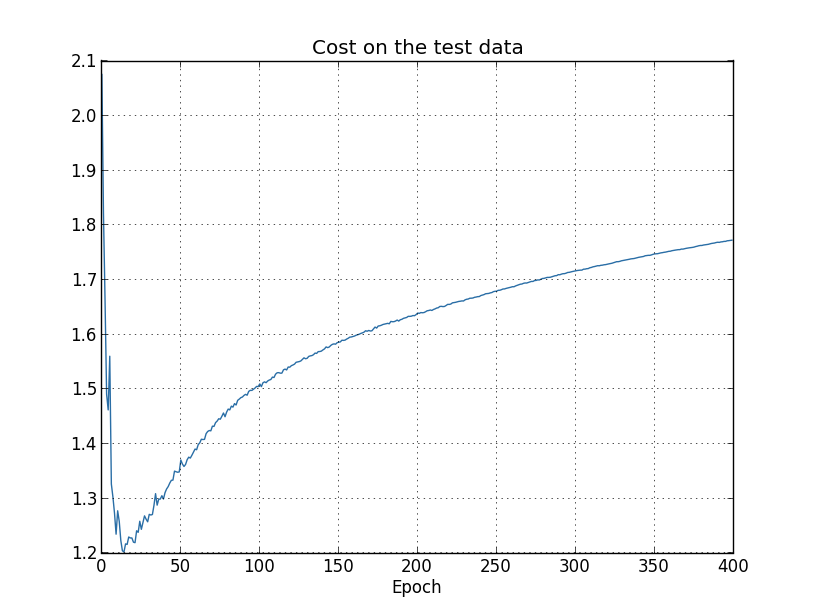
\includegraphics[width=0.6\linewidth]{figures/ch3/overfitting3}
\end{center}
We can see that the cost on the test data improves until around epoch 15, but after that it actually starts to get worse, even though the cost on the training data is continuing to get better. This is another sign that our model is overfitting. It poses a puzzle, though, which is whether we should regard epoch 15 or epoch 280 as the point at which overfitting is coming to dominate learning? From a practical point of view, what we really care about is improving classification accuracy on the test data, while the cost on the test data is no more than a proxy for classification accuracy. And so it makes most sense to regard epoch 280 as the point beyond which overfitting is dominating learning in our neural network.

Another sign of overfitting may be seen in the classification accuracy on the training data:
\begin{center}
	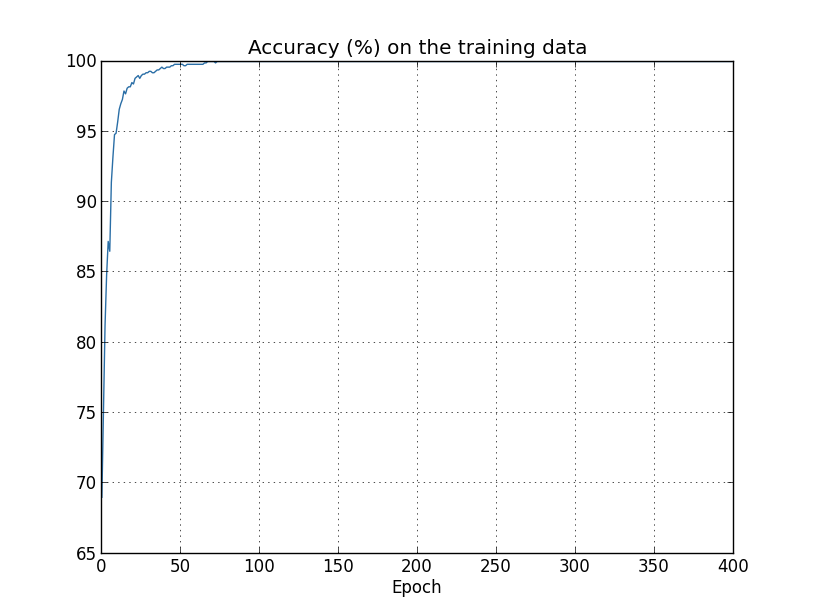
\includegraphics[width=0.6\linewidth]{figures/ch3/overfitting4}
\end{center}
The accuracy rises all the way up to 100 percent. That is, our network correctly classifies all 1,000 training images! Meanwhile, our test accuracy tops out at just 82.27 percent. So our network really is learning about peculiarities of the training set, not just recognizing digits in general. It's almost as though our network is merely memorizing the training set, without understanding digits well enough to generalize to the test set.

Overfitting is a major problem in neural networks. This is especially true in modern networks, which often have very large numbers of weights and biases. To train effectively, we need a way of detecting when overfitting is going on, so we don't overtrain. And we'd like to have techniques for reducing the effects of overfitting.

The obvious way to detect overfitting is to use the approach above, keeping track of accuracy on the test data as our network trains. If we see that the accuracy on the test data is no longer improving, then we should stop training. Of course, strictly speaking, this is not necessarily a sign of overfitting. It might be that accuracy on the test data and the training data both stop improving at the same time. Still, adopting this strategy will prevent overfitting.

In fact, we'll use a variation on this strategy. Recall that when we load in the MNIST data we load in three data sets:
\begin{lstlisting}
>>> import mnist_loader 
>>> training_data, validation_data, test_data = mnist_loader.load_data_wrapper()
\end{lstlisting}
Up to now we've been using the \inline{training_data} and \inline{test_data}, and ignoring the \texttt{validation\_data}. The \inline{validation_data} contains 10,000 images of digits, images which are different from the 50,000 images in the MNIST training set, and the 10,000 images in the MNIST test set. Instead of using the \inline{test_data} to prevent overfitting, we will use the \inline{validation_data}. To do this, we'll use much the same strategy as was described above for the \inline{test_data}. That is, we'll compute the classification accuracy on the \inline{validation_data} at the end of each epoch. Once the classification accuracy on the \inline{validation_data} has saturated, we stop training. This strategy is called early stopping. Of course, in practice we won't immediately know when the accuracy has saturated. Instead, we continue training until we're confident that the accuracy has saturated\footnote{It requires some judgment to determine when to stop. In my earlier graphs I identified epoch 280 as the place at which accuracy saturated. It's possible that was too pessimistic. Neural networks sometimes plateau for a while in training, before continuing to improve. I wouldn't be surprised if more learning could have occurred even after epoch 400, although the magnitude of any further improvement would likely be small. So it's possible to adopt more or less aggressive strategies for early stopping.}.

Why use the \inline{validation_data} to prevent overfitting, rather than the \inline{test_data}? In fact, this is part of a more general strategy, which is to use the \inline{validation_data} to evaluate different trial choices of hyper-parameters such as the number of epochs to train for, the learning rate, the best network architecture, and so on. We use such evaluations to find and set good values for the hyper-parameters. Indeed, although I haven't mentioned it until now, that is, in part, how I arrived at the hyper-parameter choices made earlier in this book. (More on this later.)

Of course, that doesn't in any way answer the question of why we're using the \texttt{validation\_data} to prevent overfitting, rather than the \inline{test_data}. Instead, it replaces it with a more general question, which is why we're using the \inline{validation_data} rather than the \inline{test_data} to set good hyper-parameters? To understand why, consider that when setting hyper-parameters we're likely to try many different choices for the hyper-parameters. If we set the hyper-parameters based on evaluations of the \inline{test_data} it's possible we'll end up overfitting our hyper-parameters to the \inline{test_data}. That is, we may end up finding hyper-parameters which fit particular peculiarities of the \inline{test_data}, but where the performance of the network won't generalize to other data sets. We guard against that by figuring out the hyper-parameters using the \inline{validation_data}. Then, once we've got the hyper-parameters we want, we do a final evaluation of accuracy using the \inline{test_data}. That gives us confidence that our results on the \inline{test_data} are a true measure of how well our neural network generalizes. To put it another way, you can think of the validation data as a type of training data that helps us learn good hyper-parameters. This approach to finding good hyper-parameters is sometimes known as the hold out method, since the \inline{validation_data} is kept apart or ``held out'' from the \inline{training_data}.

Now, in practice, even after evaluating performance on the \inline{test_data} we may change our minds and want to try another approach -- perhaps a different network architecture -- which will involve finding a new set of hyper-parameters. If we do this, isn't there a danger we'll end up overfitting to the \inline{test_data} as well? Do we need a potentially infinite regress of data sets, so we can be confident our results will generalize? Addressing this concern fully is a deep and difficult problem. But for our practical purposes, we're not going to worry too much about this question. Instead, we'll plunge ahead, using the basic hold out method, based on the \inline{training_data}, \inline{validation_data}, and \inline{test_data}, as described above.

We've been looking so far at overfitting when we're just using 1,000 training images. What happens when we use the full training set of 50,000 images? We'll keep all the other parameters the same (30 hidden neurons, learning rate 0.5, mini-batch size of 10), but train using all 50,000 images for 30 epochs. Here's a graph showing the results for the classification accuracy on both the training data and the test data. Note that I've used the test data here, rather than the validation data, in order to make the results more directly comparable with the earlier graphs.
\begin{center}
	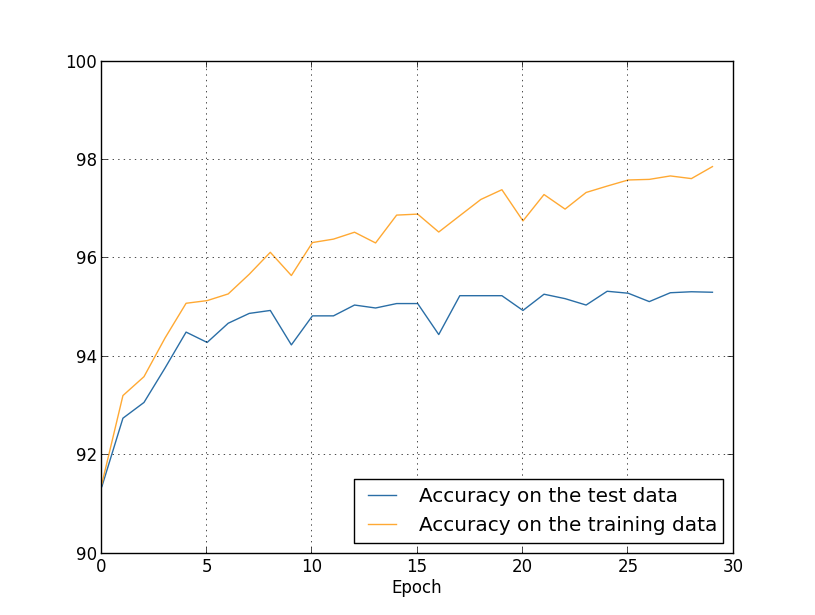
\includegraphics[width=0.6\linewidth]{figures/ch3/overfitting_full}
\end{center}
As you can see, the accuracy on the test and training data remain much closer together than when we were using 1,000 training examples. In particular, the best classification accuracy of 97.86 percent on the training data is only 2.53 percent higher than the 95.33 percent on the test data. That's compared to the 17.73 percent gap we had earlier! Overfitting is still going on, but it's been greatly reduced. Our network is generalizing much better from the training data to the test data. In general, one of the best ways of reducing overfitting is to increase the size of the training data. With enough training data it is difficult for even a very large network to overfit. Unfortunately, training data can be expensive or difficult to acquire, so this is not always a practical option.

\subsection{Regularization}
\label{sec:3.2.1}
Increasing the amount of training data is one way of reducing overfitting. Are there other ways we can reduce the extent to which overfitting occurs? One possible approach is to reduce the size of our network. However, large networks have the potential to be more powerful than small networks, and so this is an option we'd only adopt reluctantly.

Fortunately, there are other techniques which can reduce overfitting, even when we have a fixed network and fixed training data. These are known as \textit{regularization} techniques. In this section I describe one of the most commonly used regularization techniques, a technique sometimes known as \textit{weight decay} or \textit{L2 regularization}. The idea of L2 regularization is to add an extra term to the cost function, a term called the \textit{regularization term}. Here's the regularized cross-entropy:
\begin{eqnarray}
C = -\frac{1}{n} \sum_{xj} \left[ y_j \ln a^L_j+(1-y_j) \ln (1-a^L_j)\right] + \frac{\lambda}{2n} \sum_w w^2.
\label{eq:85}
\end{eqnarray}
%C=-1n∑xj[yjlnaLj+(1-yj)ln(1-aLj)]+\lambda 2n∑ww2.(85)
The first term is just the usual expression for the cross-entropy. But we've added a second term, namely the sum of the squares of all the weights in the network. This is scaled by a factor $\lambda/2n$, where $\lambda>0$ is known as the \textit{regularization parameter}, and $n$ is, as usual, the size of our training set. I'll discuss later how $\lambda$ is chosen. It's also worth noting that the regularization term doesn't include the biases. I'll also come back to that below.

Of course, it's possible to regularize other cost functions, such as the quadratic cost. This can be done in a similar way:
\begin{eqnarray} C = \frac{1}{2n} \sum_x \|y-a^L\|^2 + \frac{\lambda}{2n} \sum_w w^2.
\label{eq:86}\end{eqnarray}
%C=12n∑x∥y-aL∥2+\lambda 2n∑ww2.(86)
In both cases we can write the regularized cost function as
%C=C0+\lambda 2n∑ww2,(87)
\begin{eqnarray}  C = C_0 + \frac{\lambda}{2n}\sum_w w^2,
\label{eq:87}
\end{eqnarray}
where $C_0$ is the original, unregularized cost function.

Intuitively, the effect of regularization is to make it so the network prefers to learn small weights, all other things being equal. Large weights will only be allowed if they considerably improve the first part of the cost function. Put another way, regularization can be viewed as a way of compromising between finding small weights and minimizing the original cost function. The relative importance of the two elements of the compromise depends on the value of $\lambda$: when $\lambda$  is small we prefer to minimize the original cost function, but when $\lambda$ is large we prefer small weights.

Now, it's really not at all obvious why making this kind of compromise should help reduce overfitting! But it turns out that it does. We'll address the question of why it helps in the next section. But first, let's work through an example showing that regularization really does reduce overfitting.

To construct such an example, we first need to figure out how to apply our stochastic gradient descent learning algorithm in a regularized neural network. In particular, we need to know how to compute the partial derivatives $\partial{}C/\partial{}w$ and $\partial{}C/\partial{}b$ for all the weights and biases in the network. Taking the partial derivatives of Equation (\ref{eq:87}) gives
\begin{eqnarray} 
\frac{\partial C}{\partial w} & = & \frac{\partial C_0}{\partial w} + \frac{\lambda}{n} w \label{eq:88}\\ 
\frac{\partial C}{\partial b} & = & \frac{\partial C_0}{\partial b}. \label{eq:89}\end{eqnarray}
%\partial{}C\partial{}w\partial{}C\partial{}b==\partial{}C0\partial{}w+\lambda nw\partial{}C0\partial{}b.(88)(89)
The $\partial{}C_0/\partial{}w$ and $\partial{}C_0/\partial{}b$ terms can be computed using backpropagation, as described in the last chapter. And so we see that it's easy to compute the gradient of the regularized cost function: just use backpropagation, as usual, and then add $\frac{\lambda}{n}w$ to the partial derivative of all the weight terms. The partial derivatives with respect to the biases are unchanged, and so the gradient descent learning rule for the biases doesn't change from the usual rule:
\begin{equation}
b\to b-\eta\frac{\partial{}C_0}{\partial{}b}.
\label{eq:90}
\end{equation}
The learning rule for the weights becomes:
\begin{eqnarray} 
w & \rightarrow & w-\eta \frac{\partial C_0}{\partial w}-\frac{\eta \lambda}{n} w  = \left(1-\frac{\eta \lambda}{n}\right) w -\eta \frac{\partial	C_0}{\partial w}. 
\label{eq:92}
\end{eqnarray}
%w→=w-\eta\partial{}C0\partial{}w-\eta\lambda nw(1-\eta\lambda n)w-\eta\partial{}C0\partial{}w.(91)(92)
This is exactly the same as the usual gradient descent learning rule, except we first rescale the weight $w$ by a factor $1-\eta\frac{\lambda}{n}$. This rescaling is sometimes referred to as \textit{weight decay}, since it makes the weights smaller. At first glance it looks as though this means the weights are being driven unstoppably toward zero. But that's not right, since the other term may lead the weights to increase, if so doing causes a decrease in the unregularized cost function.

Okay, that's how gradient descent works. What about stochastic gradient descent? Well, just as in unregularized stochastic gradient descent, we can estimate $\partial{}C_0/\partial{}w$ by averaging over a mini-batch of $m$ training examples. Thus the regularized learning rule for stochastic gradient descent becomes (c.f. Equation (\ref{eq:20}))
\begin{eqnarray} 
w \rightarrow \left(1-\frac{\eta \lambda}{n}\right) w -\frac{\eta}{m} \sum_x \frac{\partial C_x}{\partial w}, 
\label{eq:93}
\end{eqnarray}
%w→(1-\eta\lambda n)w-\etam∑x\partial{}Cx\partial{}w,(93)
where the sum is over training examples $x$ in the mini-batch, and $C_x$ is the (unregularized) cost for each training example. This is exactly the same as the usual rule for stochastic gradient descent, except for the $1-\eta\lambda/n$ weight decay factor. Finally, and for completeness, let me state the regularized learning rule for the biases. This is, of course, exactly the same as in the unregularized case (c.f. Equation \ref{eq:21}),
\begin{eqnarray}
	b \to b - \frac{\eta}{m} \sum_x \frac{\partial C_x}{\partial b},
	\label{eq:94}
\end{eqnarray}
%b→b-\etam∑x\partial{}Cx\partial{}b,(94)
where the sum is over training examples $x$ in the mini-batch.

Let's see how regularization changes the performance of our neural network. We'll use a network with 30 hidden neurons, a mini-batch size of 10, a learning rate of 0.5, and the cross-entropy cost function. However, this time we'll use a regularization parameter of $\lambda =0.1$. Note that in the code, we use the variable name \inline{lmbda}, because \inline{lambda} is a reserved word in Python, with an unrelated meaning. I've also used the \inline{test_data} again, not the \inline{validation_data}. Strictly speaking, we should use the \inline{validation_data}, for all the reasons we discussed earlier. But I decided to use the \inline{test_data} because it makes the results more directly comparable with our earlier, unregularized results. You can easily change the code to use the \inline{validation_data} instead, and you'll find that it gives similar results.

\begin{lstlisting}

>>> import mnist_loader 
>>> training_data, validation_data, test_data =  mnist_loader.load_data_wrapper() 
>>> import network2 
>>> net = network2.Network([784, 30, 10], cost=network2.CrossEntropyCost)
>>> net.large_weight_initializer()
>>> net.SGD(training_data[:1000], 400, 10, 0.5, evaluation_data=test_data, lmbda = 0.1, \
... monitor_evaluation_cost=True, monitor_evaluation_accuracy=True, monitor_training_cost=True, monitor_training_accuracy=True)
\end{lstlisting}
The cost on the training data decreases over the whole time, much as it did in the earlier, unregularized case\footnote{This and the next two graphs were produced with the program \inline{overfitting.py.}}:
\begin{center}
	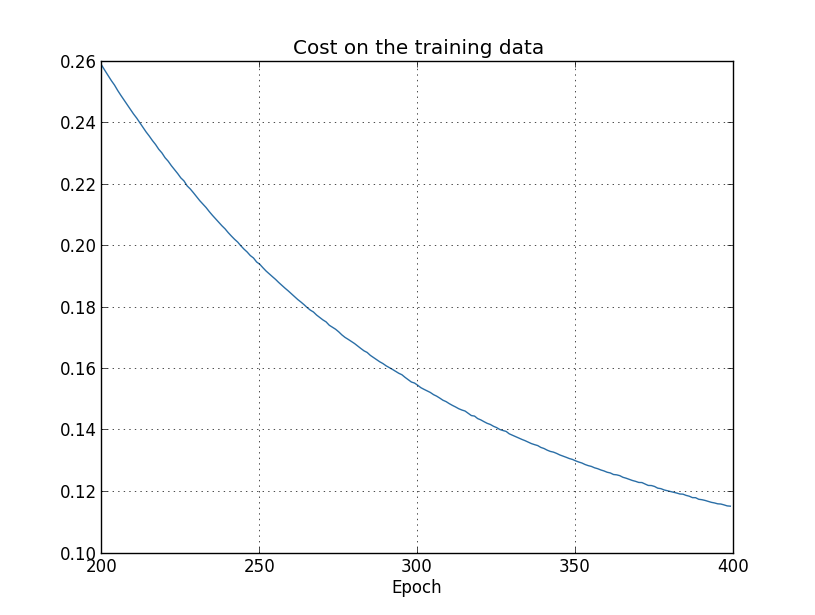
\includegraphics[width=0.6\linewidth]{figures/ch3/regularized1}
\end{center}
But this time the accuracy on the \inline{test_data} continues to increase for the entire 400 epochs:
\begin{center}
	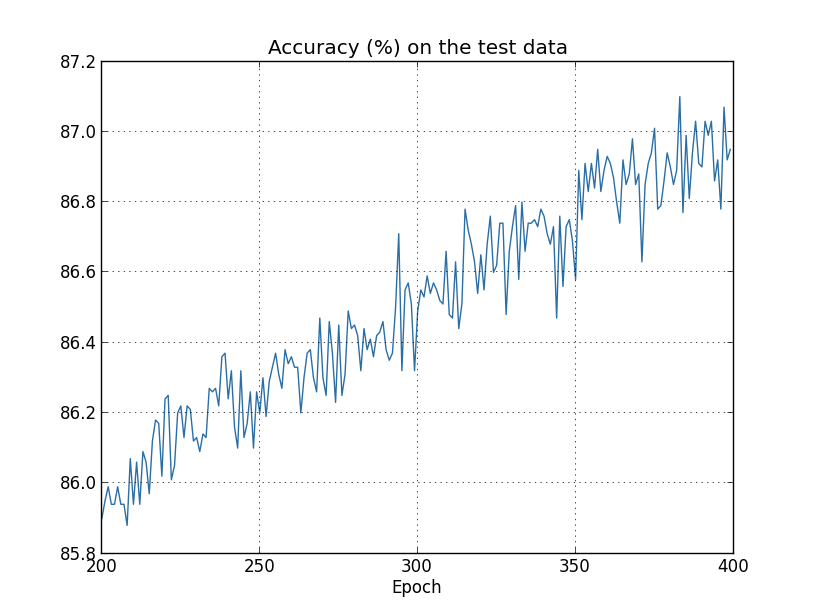
\includegraphics[width=0.6\linewidth]{figures/ch3/regularized2}
\end{center}
Clearly, the use of regularization has suppressed overfitting. What's more, the accuracy is considerably higher, with a peak classification accuracy of 87.1 percent, compared to the peak of 82.27 percent obtained in the unregularized case. Indeed, we could almost certainly get considerably better results by continuing to train past 400 epochs. It seems that, empirically, regularization is causing our network to generalize better, and considerably reducing the effects of overfitting.

What happens if we move out of the artificial environment of just having 1,000 training images, and return to the full 50,000 image training set? Of course, we've seen already that overfitting is much less of a problem with the full 50,000 images. Does regularization help any further? Let's keep the hyper-parameters the same as before -- 30 epochs, learning rate 0.5, mini-batch size of 10. However, we need to modify the regularization parameter. The reason is because the size $n$ of the training set has changed from $n$=1,000 to $n$=50,000, and this changes the weight decay factor $1-\eta\lambda/n$. If we continued to use $\lambda =0.1$ that would mean much less weight decay, and thus much less of a regularization effect. We compensate by changing to $\lambda =5.0$.

Okay, let's train our network, stopping first to re-initialize the weights:

\begin{lstlisting}
>>> net.large_weight_initializer()
>>> net.SGD(training_data, 30, 10, 0.5, evaluation_data=test_data, lmbda = 5.0,
... monitor_evaluation_accuracy=True, monitor_training_accuracy=True)
\end{lstlisting}
We obtain the results:
\begin{center}
	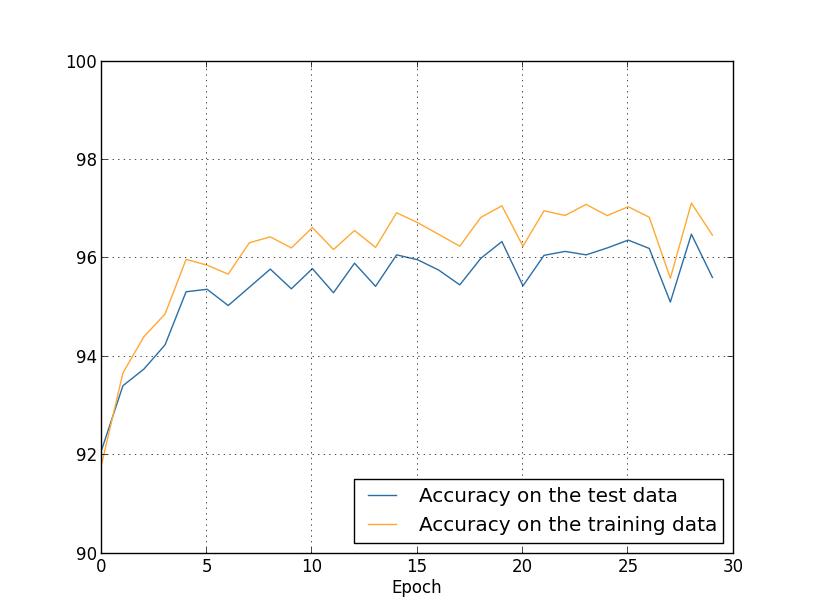
\includegraphics[width=0.6\linewidth]{figures/ch3/regularized_full}
\end{center}
There's lots of good news here. First, our classification accuracy on the test data is up, from 95.49 percent when running unregularized, to 96.49 percent. That's a big improvement. Second, we can see that the gap between results on the training and test data is much narrower than before, running at under a percent. That's still a significant gap, but we've obviously made substantial progress reducing overfitting.


Finally, let's see what test classification accuracy we get when we use 100 hidden neurons and a regularization parameter of $\lambda =5.0$. I won't go through a detailed analysis of overfitting here, this is purely for fun, just to see how high an accuracy we can get when we use our new tricks: the cross-entropy cost function and L2 regularization.

\begin{lstlisting}

>>> net = network2.Network([784, 100, 10], cost=network2.CrossEntropyCost)
>>> net.large_weight_initializer()
>>> net.SGD(training_data, 30, 10, 0.5, lmbda=5.0, evaluation_data=validation_data,
... monitor_evaluation_accuracy=True)

\end{lstlisting}
The final result is a classification accuracy of 97.92 percent on the validation data. That's a big jump from the 30 hidden neuron case. In fact, tuning just a little more, to run for 60 epochs at $\eta=0.1$ and $\lambda =5.0$ we break the 98 percent barrier, achieving 98.04 percent classification accuracy on the validation data. Not bad for what turns out to be 152 lines of code!

I've described regularization as a way to reduce overfitting and to increase classification accuracies. In fact, that's not the only benefit. Empirically, when doing multiple runs of our MNIST networks, but with different (random) weight initializations, I've found that the unregularized runs will occasionally get ``stuck'', apparently caught in local minima of the cost function. The result is that different runs sometimes provide quite different results. By contrast, the regularized runs have provided much more easily replicable results.

Why is this going on? Heuristically, if the cost function is unregularized, then the length of the weight vector is likely to grow, all other things being equal. Over time this can lead to the weight vector being very large indeed. This can cause the weight vector to get stuck pointing in more or less the same direction, since changes due to gradient descent only make tiny changes to the direction, when the length is long. I believe this phenomenon is making it hard for our learning algorithm to properly explore the weight space, and consequently harder to find good minima of the cost function.


\subsection{Why does regularization help reduce overfitting?}
We've seen empirically that regularization helps reduce overfitting. That's encouraging but, unfortunately, it's not obvious why regularization helps! A standard story people tell to explain what's going on is along the following lines: smaller weights are, in some sense, lower complexity, and so provide a simpler and more powerful explanation for the data, and should thus be preferred. That's a pretty terse story, though, and contains several elements that perhaps seem dubious or mystifying. Let's unpack the story and examine it critically. To do that, let's suppose we have a simple data set for which we wish to build a model:
\begin{center}
\begin{tikzpicture}
\begin{axis}[xmin=0,xmax=5.5,ymin=0,ymax=11,xlabel={$x$},ylabel={$y$},width=0.85\linewidth,height=0.5\linewidth]
	\addplot[only marks,blue!65!green!75] coordinates {( 0.7, 1.8) ( 1.3, 2.2)   ( 1.9, 4.0) ( 2.6, 5.0)  ( 2.9, 6.1) ( 3.6, 7.0) ( 3.8, 7.4)   ( 3.95, 8.0)   ( 4.4, 9.1)  ( 4.9, 10.0)};
\end{axis}
\end{tikzpicture}
\end{center}
%\begin{center}
%	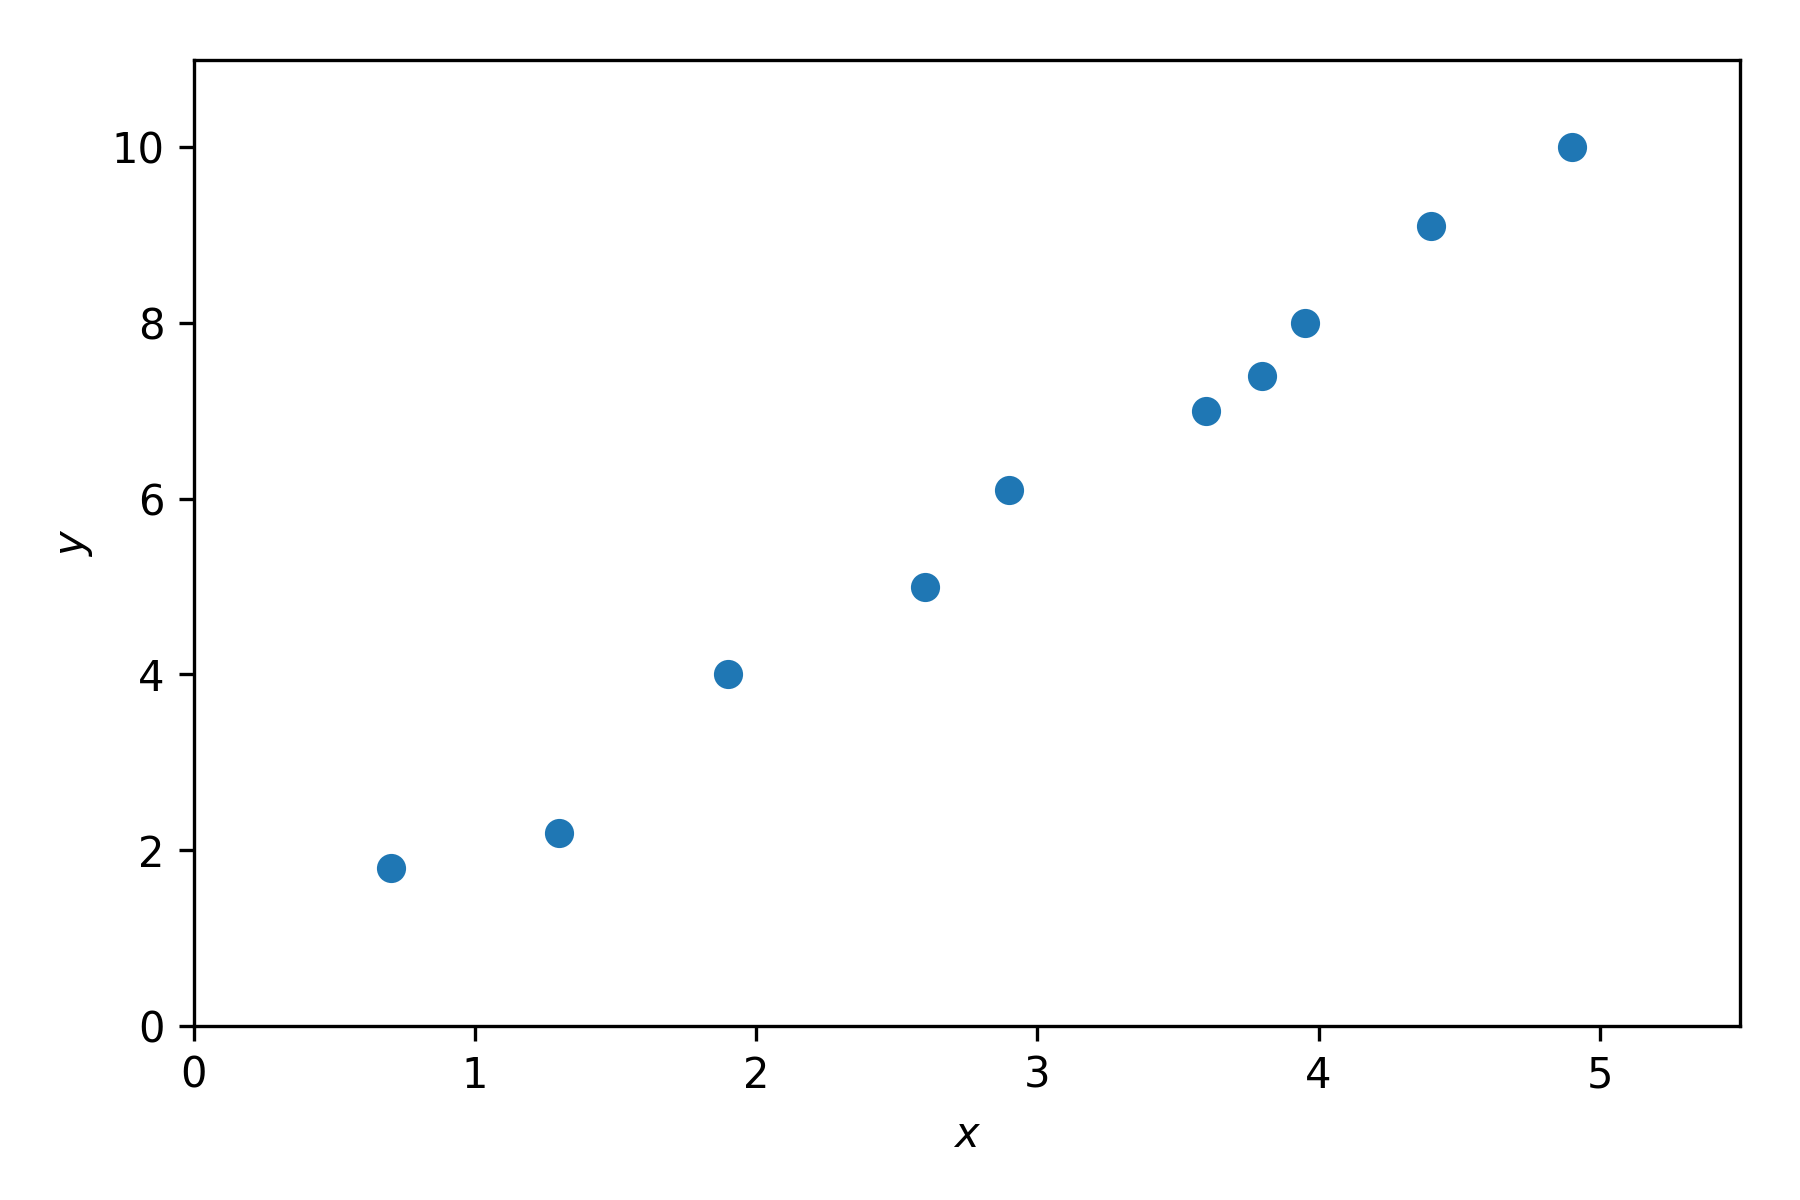
\includegraphics[width=0.7\linewidth]{figures/ch3/animation_overfitting1}
%\end{center}
Implicitly, we're studying some real-world phenomenon here, with $x$ and $y$ representing real-world data. Our goal is to build a model which lets us predict $y$ as a function of $x$. We could try using neural networks to build such a model, but I'm going to do something even simpler: I'll try to model $y$ as a polynomial in $x$. I'm doing this instead of using neural nets because using polynomials will make things particularly transparent. Once we've understood the polynomial case, we'll translate to neural networks. Now, there are ten points in the graph above, which means we can find a unique 9-th-order polynomial $y=a_0x^9+a_1x^8+\ldots+a_9$ which fits the data exactly. Here's the graph of that polynomial\footnote{I won't show the coefficients explicitly, although they are easy to find using a routine such as Numpy's \inline{polyfit}.You can view the exact form of the polynomial in the \href{http://neuralnetworksanddeeplearning.com/js/polynomial_model.js}{source code for the graph} if you're curious. It's the function $p(x)$ defined starting on line 14 of the program which produces the graph.} :
\begin{center}
\begin{tikzpicture}
% here the code as a bit hacked, since pgfplots badly behaves at large numbers, and causes a lot of rounding errors. That's why first points were centered around 0, interpolated, and than paramaters from the interpolation are taken
\begin{axis}[xmin=0,xmax=5.5,ymin=0,ymax=11,xlabel={$x$},ylabel={$y$},width=0.85\linewidth,height=0.5\linewidth]
	\addplot[only marks,blue!65!green!75] coordinates {( 0.7, 1.8) ( 1.3, 2.2)   ( 1.9, 4.0) ( 2.6, 5.0)  ( 2.9, 6.1) ( 3.6, 7.0) ( 3.8, 7.4)   ( 3.95, 8.0)   ( 4.4, 9.1)  ( 4.9, 10.0)};
	\addplot[domain=0.6:5.0,samples=163,black] {((((((((0.22054*(x-2.8)+0.066159)*(x-2.8)-1.9786)*(x-2.8)-0.5296)*(x-2.8)+5.6811)*(x-2.8)+1.26589)*(x-2.8)-5.896288)*(x-2.8)-0.92050732)*(x-2.8)+3.751559)*(x-2.8)+5.73976};
\end{axis}
\end{tikzpicture}
\end{center}
%\begin{center}
%	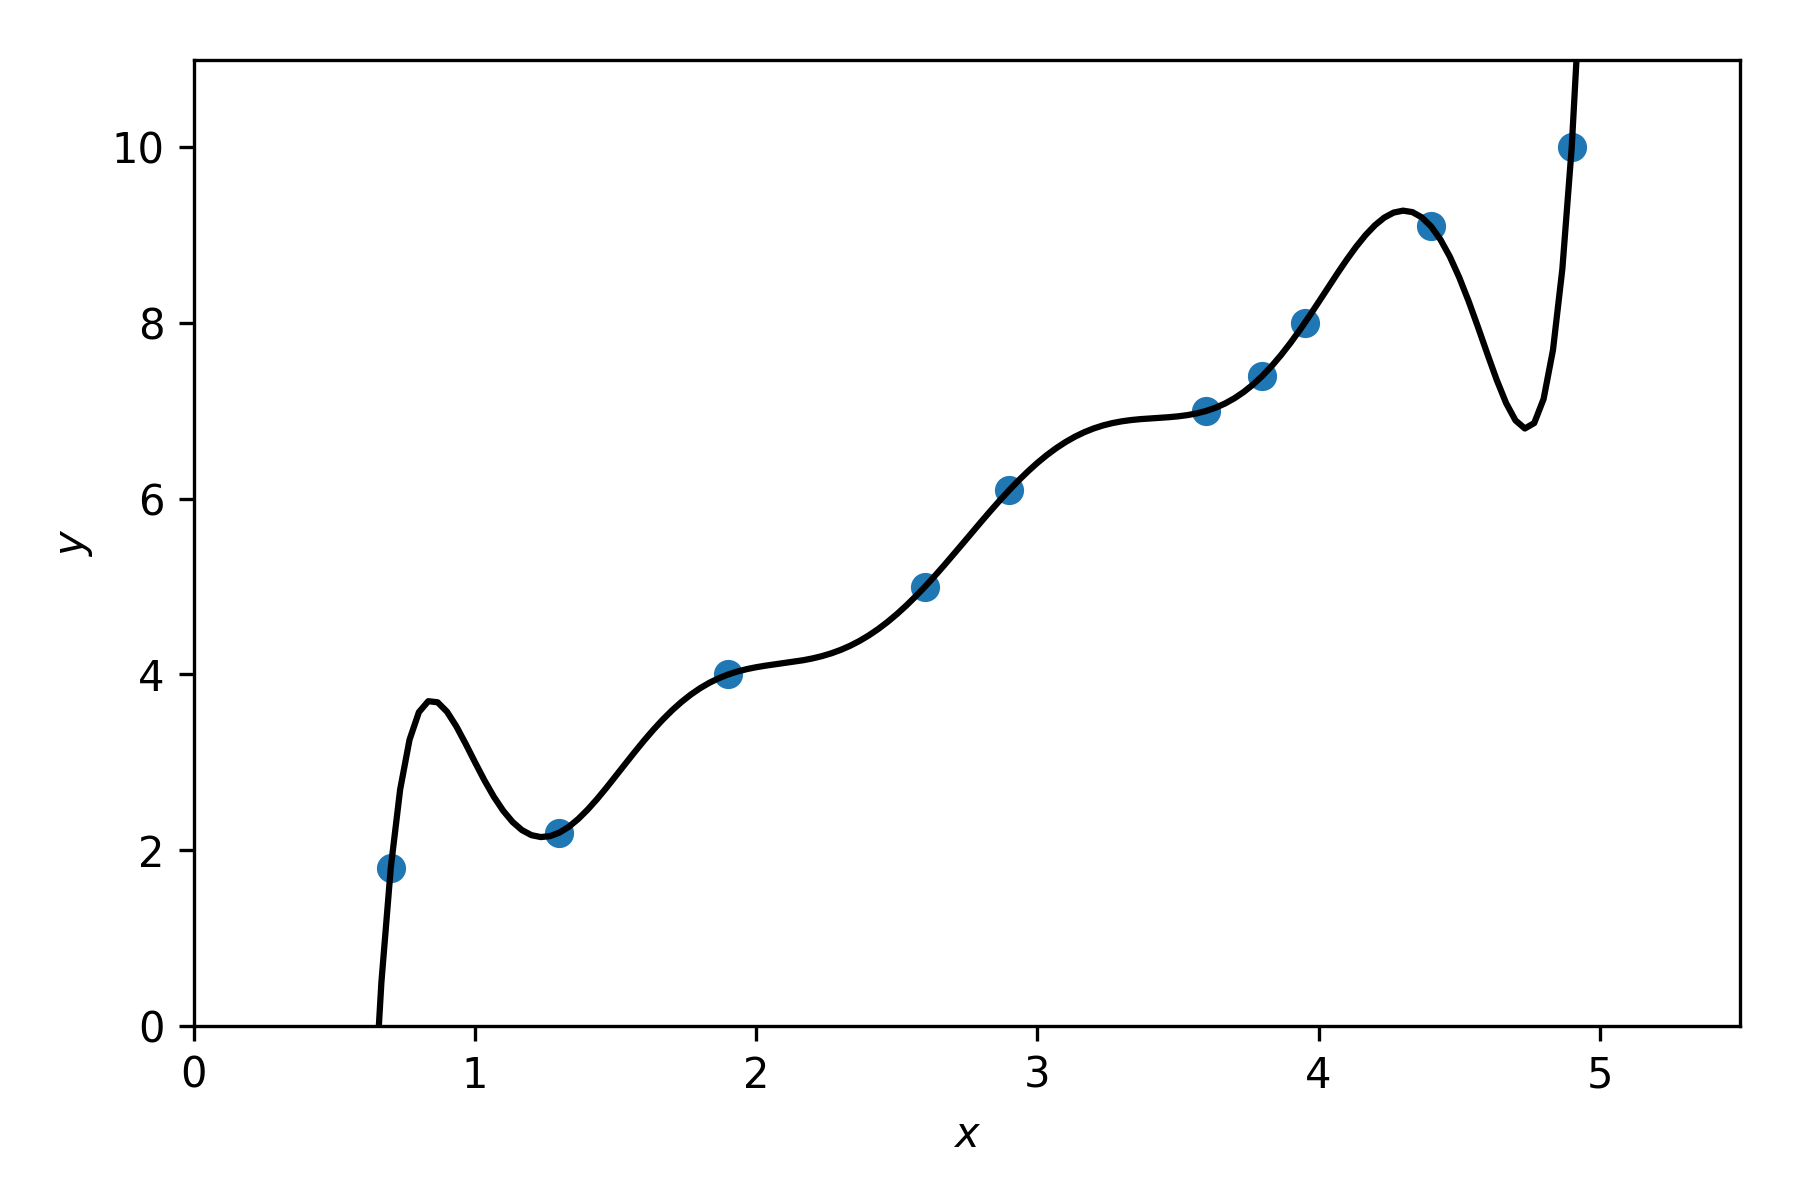
\includegraphics[width=0.7\linewidth]{figures/ch3/animation_overfitting2}
%	\end{center}
That provides an exact fit. But we can also get a good fit using the linear model $y=2x$:
\begin{center}
\begin{tikzpicture}
\begin{axis}[xmin=0,xmax=5.5,ymin=0,ymax=11,xlabel={$x$},ylabel={$y$},width=0.85\linewidth,height=0.5\linewidth]
	\addplot[only marks,blue!65!green!75] coordinates {( 0.7, 1.8) ( 1.3, 2.2)   ( 1.9, 4.0) ( 2.6, 5.0)  ( 2.9, 6.1) ( 3.6, 7.0) ( 3.8, 7.4)   ( 3.95, 8.0)   ( 4.4, 9.1)  ( 4.9, 10.0)};
	\addplot[domain=0:5.5,samples=111,black] {2*x};
\end{axis}
\end{tikzpicture}
\end{center}
%\begin{center}
%	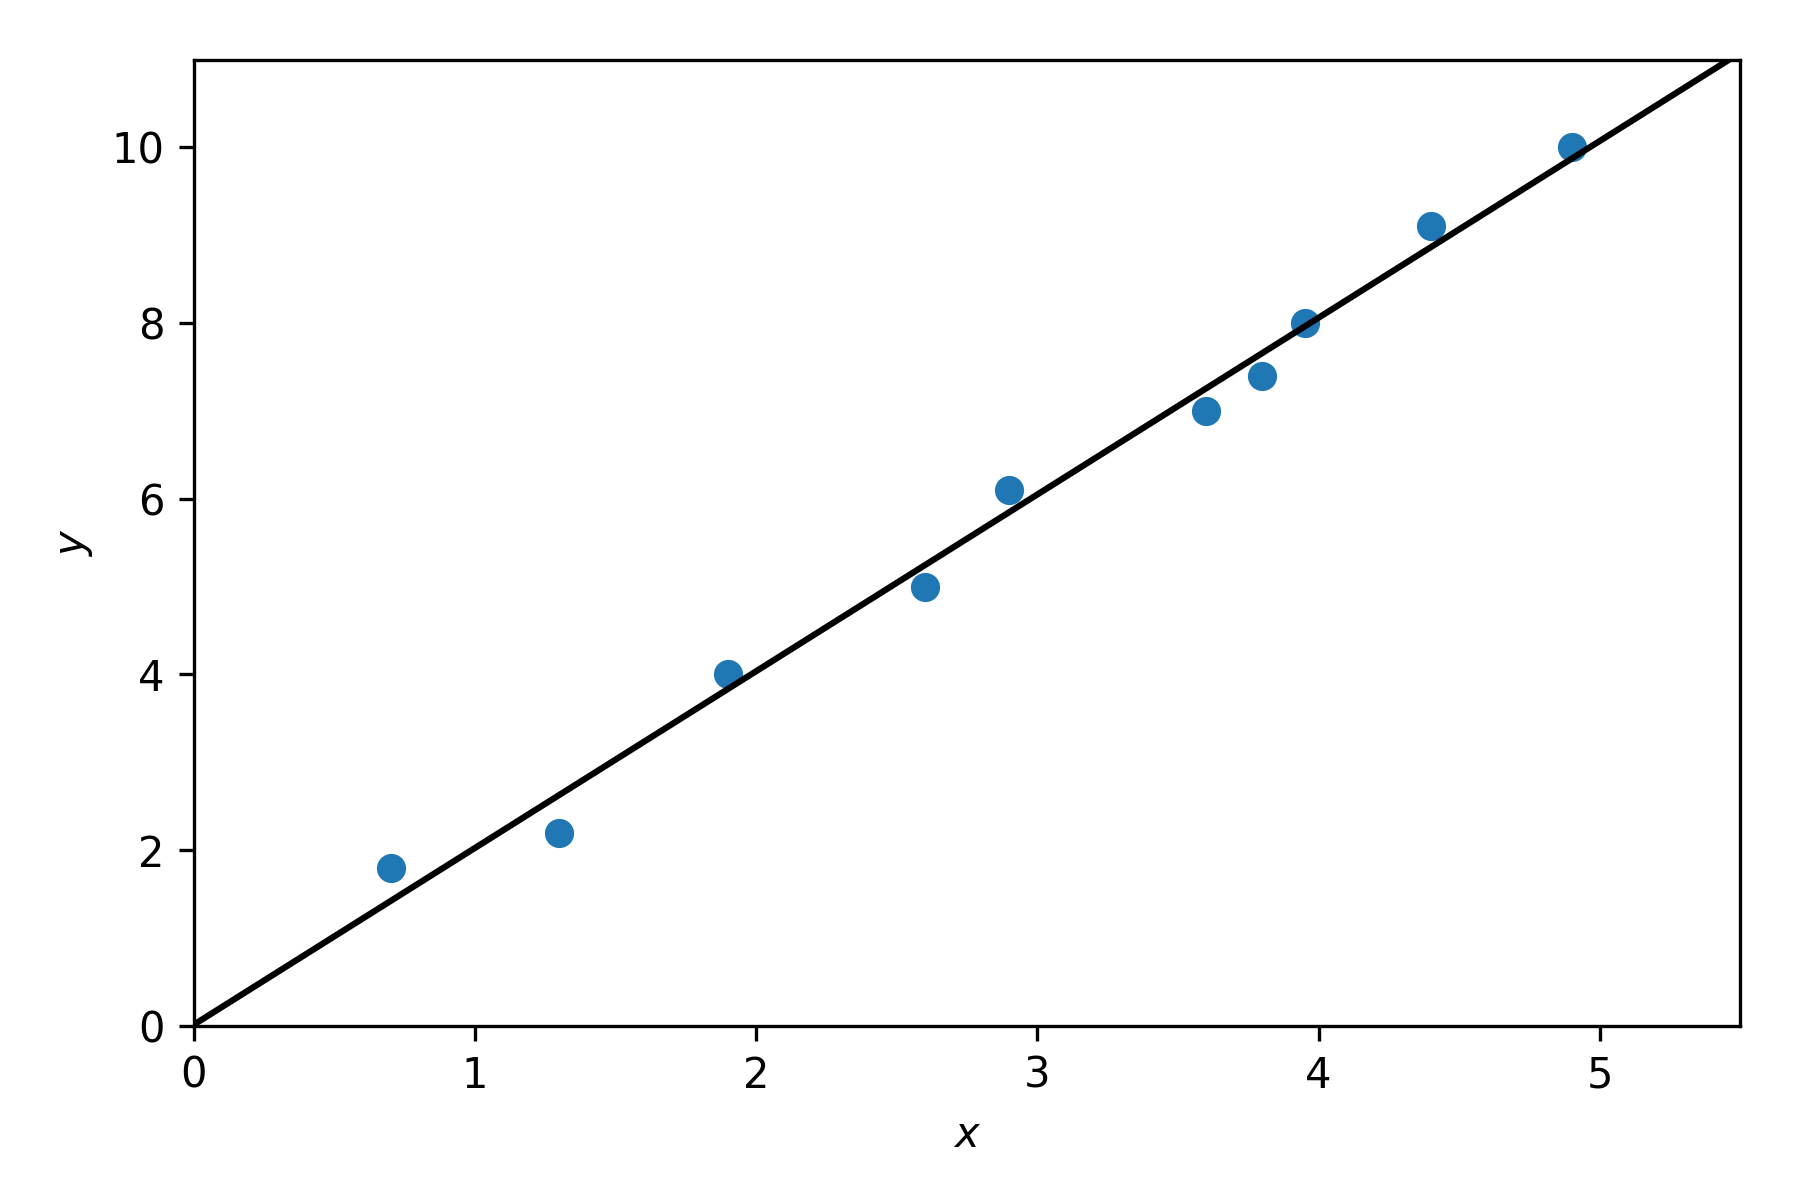
\includegraphics[width=0.7\linewidth]{figures/ch3/animation_overfitting3}
%\end{center}
Which of these is the better model? Which is more likely to be true? And which model is more likely to generalize well to other examples of the same underlying real-world phenomenon?

These are difficult questions. In fact, we can't determine with certainty the answer to any of the above questions, without much more information about the underlying real-world phenomenon. But let's consider two possibilities: (1) the 9th order polynomial is, in fact, the model which truly describes the real-world phenomenon, and the model will therefore generalize perfectly; (2) the correct model is $y=2x$, but there's a little additional noise due to, say, measurement error, and that's why the model isn't an exact fit.

It's not \textit{a priori} possible to say which of these two possibilities is correct. (Or, indeed, if some third possibility holds). Logically, either could be true. And it's not a trivial difference. It's true that on the data provided there's only a small difference between the two models. But suppose we want to predict the value of $y$ corresponding to some large value of $x$, much larger than any shown on the graph above. If we try to do that there will be a dramatic difference between the predictions of the two models, as the 9th order polynomial model comes to be dominated by the $x^9$ term, while the linear model remains, well, linear.

One point of view is to say that in science we should go with the simpler explanation, unless compelled not to. When we find a simple model that seems to explain many data points we are tempted to shout ``Eureka!'' After all, it seems unlikely that a simple explanation should occur merely by coincidence. Rather, we suspect that the model must be expressing some underlying truth about the phenomenon. In the case at hand, the model $y=2x+{\rm noise}$ seems much simpler than $y=a_0x^9+a_1x^8+\ldots$. It would be surprising if that simplicity had occurred by chance, and so we suspect that $y=2x+{\rm noise}$ expresses some underlying truth. In this point of view, the 9th order model is really just learning the effects of local noise. And so while the 9th order model works perfectly for these particular data points, the model will fail to generalize to other data points, and the noisy linear model will have greater predictive power.

Let's see what this point of view means for neural networks. Suppose our network mostly has small weights, as will tend to happen in a regularized network. The smallness of the weights means that the behaviour of the network won't change too much if we change a few random inputs here and there. That makes it difficult for a regularized network to learn the effects of local noise in the data. Think of it as a way of making it so single pieces of evidence don't matter too much to the output of the network. Instead, a regularized network learns to respond to types of evidence which are seen often across the training set. By contrast, a network with large weights may change its behaviour quite a bit in response to small changes in the input. And so an unregularized network can use large weights to learn a complex model that carries a lot of information about the noise in the training data. In a nutshell, regularized networks are constrained to build relatively simple models based on patterns seen often in the training data, and are resistant to learning peculiarities of the noise in the training data. The hope is that this will force our networks to do real learning about the phenomenon at hand, and to generalize better from what they learn.

With that said, this idea of preferring simpler explanation should make you nervous. People sometimes refer to this idea as ``Occam's Razor'', and will zealously apply it as though it has the status of some general scientific principle. But, of course, it's not a general scientific principle. There is no \textit{a priori} logical reason to prefer simple explanations over more complex explanations. Indeed, sometimes the more complex explanation turns out to be correct.

Let me describe two examples where more complex explanations have turned out to be correct. In the 1940s the physicist Marcel Schein announced the discovery of a new particle of nature. The company he worked for, General Electric, was ecstatic, and publicized the discovery widely. But the physicist Hans Bethe was skeptical. Bethe visited Schein, and looked at the plates showing the tracks of Schein's new particle. Schein showed Bethe plate after plate, but on each plate Bethe identified some problem that suggested the data should be discarded. Finally, Schein showed Bethe a plate that looked good. Bethe said it might just be a statistical fluke. Schein: ``Yes, but the chance that this would be statistics, even according to your own formula, is one in five.'' Bethe: ``But we have already looked at five plates.'' Finally, Schein said: ``But on my plates, each one of the good plates, each one of the good pictures, you explain by a different theory, whereas I have one hypothesis that explains all the plates, that they are [the new particle].'' Bethe replied: ``The sole difference between your and my explanations is that yours is wrong and all of mine are right. Your single explanation is wrong, and all of my multiple explanations are right.'' Subsequent work confirmed that Nature agreed with Bethe, and Schein's particle is no more\footnote{The story is related by the physicist Richard Feynman in an \href{https://www.aip.org/history-programs/niels-bohr-library/oral-histories/5020-4}{interview} with the historian Charles Weiner.}.

As a second example, in 1859 the astronomer Urbain Le Verrier observed that the orbit of the planet Mercury doesn't have quite the shape that Newton's theory of gravitation says it should have. It was a tiny, tiny deviation from Newton's theory, and several of the explanations proferred at the time boiled down to saying that Newton's theory was more or less right, but needed a tiny alteration. In 1916, Einstein showed that the deviation could be explained very well using his general theory of relativity, a theory radically different to Newtonian gravitation, and based on much more complex mathematics. Despite that additional complexity, today it's accepted that Einstein's explanation is correct, and Newtonian gravity, even in its modified forms, is wrong. This is in part because we now know that Einstein's theory explains many other phenomena which Newton's theory has difficulty with. Furthermore, and even more impressively, Einstein's theory accurately predicts several phenomena which aren't predicted by Newtonian gravity at all. But these impressive qualities weren't entirely obvious in the early days. If one had judged merely on the grounds of simplicity, then some modified form of Newton's theory would arguably have been more attractive.

There are three morals to draw from these stories. First, it can be quite a subtle business deciding which of two explanations is truly ``simpler''. Second, even if we can make such a judgment, simplicity is a guide that must be used with great caution! Third, the true test of a model is not simplicity, but rather how well it does in predicting new phenomena, in new regimes of behaviour.

With that said, and keeping the need for caution in mind, it's an empirical fact that regularized neural networks usually generalize better than unregularized networks. And so through the remainder of the book we will make frequent use of regularization. I've included the stories above merely to help convey why no-one has yet developed an entirely convincing theoretical explanation for why regularization helps networks generalize. Indeed, researchers continue to write papers where they try different approaches to regularization, compare them to see which works better, and attempt to understand why different approaches work better or worse. And so you can view regularization as something of a kludge. While it often helps, we don't have an entirely satisfactory systematic understanding of what's going on, merely incomplete heuristics and rules of thumb.

There's a deeper set of issues here, issues which go to the heart of science. It's the question of how we generalize. Regularization may give us a computational magic wand that helps our networks generalize better, but it doesn't give us a principled understanding of how generalization works, nor of what the best approach is\footnote{These issues go back to the \href{http://en.wikipedia.org/wiki/Problem_of_induction}{problem of induction}, famously discussed by the Scottish philosopher David Hume in \href{http://www.gutenberg.org/ebooks/9662}{``An Enquiry Concerning Human Understanding''} (1748). The problem of induction has been given a modern machine learning form in the \href{http://ieeexplore.ieee.org/xpl/articleDetails.jsp?tp=&arnumber=585893}{no-free lunch theorem} of David Wolpert and William Macready (1997).}.

This is particularly galling because in everyday life, we humans generalize phenomenally well. Shown just a few images of an elephant a child will quickly learn to recognize other elephants. Of course, they may occasionally make mistakes, perhaps confusing a rhinoceros for an elephant, but in general this process works remarkably accurately. So we have a system -- the human brain -- with a huge number of free parameters. And after being shown just one or a few training images that system learns to generalize to other images. Our brains are, in some sense, regularizing amazingly well! How do we do it? At this point we don't know. I expect that in years to come we will develop more powerful techniques for regularization in artificial neural networks, techniques that will ultimately enable neural nets to generalize well even from small data sets.

In fact, our networks already generalize better than one might a priori expect. A network with 100 hidden neurons has nearly 80,000 parameters. We have only 50,000 images in our training data. It's like trying to fit an 80,000th degree polynomial to 50,000 data points. By all rights, our network should overfit terribly. And yet, as we saw earlier, such a network actually does a pretty good job generalizing. Why is that the case? It's not well understood. It has been conjectured\footnote{In \href{http://yann.lecun.com/exdb/publis/pdf/lecun-01a.pdf}{Gradient-Based Learning Applied to Document Recognition}, by Yann LeCun, L\'{e}on Bottou, Yoshua Bengio, and Patrick Haffner (1998).} that ``the dynamics of gradient descent learning in multilayer nets has a `self-regularization' effect''. This is exceptionally fortunate, but it's also somewhat disquieting that we don't understand why it's the case. In the meantime, we will adopt the pragmatic approach and use regularization whenever we can. Our neural networks will be the better for it.

Let me conclude this section by returning to a detail which I left unexplained earlier: the fact that L2 regularization doesn't constrain the biases. Of course, it would be easy to modify the regularization procedure to regularize the biases. Empirically, doing this often doesn't change the results very much, so to some extent it's merely a convention whether to regularize the biases or not. However, it's worth noting that having a large bias doesn't make a neuron sensitive to its inputs in the same way as having large weights. And so we don't need to worry about large biases enabling our network to learn the noise in our training data. At the same time, allowing large biases gives our networks more flexibility in behaviour -- in particular, large biases make it easier for neurons to saturate, which is sometimes desirable. For these reasons we don't usually include bias terms when regularizing.


\subsection{Other techniques for regularization}
There are many regularization techniques other than L2 regularization. In fact, so many techniques have been developed that I can't possibly summarize them all. In this section I briefly describe three other approaches to reducing overfitting: L1 regularization, dropout, and artificially increasing the training set size. We won't go into nearly as much depth studying these techniques as we did earlier. Instead, the purpose is to get familiar with the main ideas, and to appreciate something of the diversity of regularization techniques available.

\textbf{L1 regularization:} In this approach we modify the unregularized cost function by adding the sum of the absolute values of the weights:
\begin{eqnarray}  C = C_0 + \frac{\lambda}{n} \sum_w |w|.\label{eq:95}
\end{eqnarray}
%C=C0+\lambdan∑w|w|.(95)
Intuitively, this is similar to L2 regularization, penalizing large weights, and tending to make the network prefer small weights. Of course, the L1 regularization term isn't the same as the L2 regularization term, and so we shouldn't expect to get exactly the same behaviour. Let's try to understand how the behaviour of a network trained using L1 regularization differs from a network trained using L2 regularization.

To do that, we'll look at the partial derivatives of the cost function. Differentiating (95) we obtain:
\begin{eqnarray}
\frac{\partial C}{\partial w} = \frac{\partial C_0}{\partial w} + \frac{\lambda}{n} \, {\rm sgn}(w),\label{eq:96}
\end{eqnarray}
%\partial{}C\partial{}w=\partial{}C0\partial{}w+\lambdansgn(w),(96)
where ${\rm sgn}(w)$ is the sign of $w$, that is, $+1$ if $w$ is positive, and $-1$ if $w$ is negative. Using this expression, we can easily modify backpropagation to do stochastic gradient descent using L1 regularization. The resulting update rule for an L1 regularized network is
\begin{eqnarray}  w \to w' = w-\frac{\eta \lambda}{n} \mbox{sgn}(w) - \eta \frac{\partial C_0}{\partial w}, \label{eq:97}\end{eqnarray}
%w→w′=w-\eta\lambdansgn(w)-\eta\partial{}C0\partial{}w,(97)
where, as per usual, we can estimate $\partial{}C_0/\partial{}w$ using a mini-batch average, if we wish. Compare that to the update rule for L2 regularization (c.f. Equation (\ref{eq:93})),
\begin{eqnarray}
w \to w' = w\left(1 - \frac{\eta \lambda}{n} \right) - \eta \frac{\partial C_0}{\partial w}.
\label{eq:98}\end{eqnarray}
%w→w′=w(1-\eta\lambdan)-\eta\partial{}C0\partial{}w.(98)
In both expressions the effect of regularization is to shrink the weights. This accords with our intuition that both kinds of regularization penalize large weights. But the way the weights shrink is different. In L1 regularization, the weights shrink by a constant amount toward 0. In L2 regularization, the weights shrink by an amount which is proportional to $w$. And so when a particular weight has a large magnitude, $|w|$, L1 regularization shrinks the weight much less than L2 regularization does. By contrast, when $|w|$ is small, L1 regularization shrinks the weight much more than L2 regularization. The net result is that L1 regularization tends to concentrate the weight of the network in a relatively small number of high-importance connections, while the other weights are driven toward zero.

I've glossed over an issue in the above discussion, which is that the partial derivative $\partial{}C/\partial{}w$ isn't defined when $w=0$. The reason is that the function $|w|$ has a sharp ``corner'' at $w=0$, and so isn't differentiable at that point. That's okay, though. What we'll do is just apply the usual (unregularized) rule for stochastic gradient descent when $w=0$. That should be okay -- intuitively, the effect of regularization is to shrink weights, and obviously it can't shrink a weight which is already 0. To put it more precisely, we'll use Equations (\ref{eq:96}) and (\ref{eq:97}) with the convention that ${\rm sgn}(0)=0$. That gives a nice, compact rule for doing stochastic gradient descent with L1 regularization.

\textbf{Dropout:} Dropout is a radically different technique for regularization. Unlike L1 and L2 regularization, dropout doesn't rely on modifying the cost function. Instead, in dropout we modify the network itself. Let me describe the basic mechanics of how dropout works, before getting into why it works, and what the results are.

Suppose we're trying to train a network:
\begin{center}
	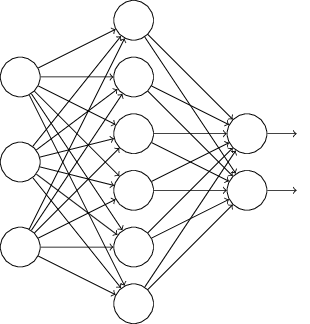
\includegraphics[width=0.45\linewidth]{figures/ch3/tikz30}
\end{center}
In particular, suppose we have a training input $x$ and corresponding desired output $y$. Ordinarily, we'd train by forward-propagating $x$ through the network, and then backpropagating to determine the contribution to the gradient. With dropout, this process is modified. We start by randomly (and temporarily) deleting half the hidden neurons in the network, while leaving the input and output neurons untouched. After doing this, we'll end up with a network along the following lines. Note that the dropout neurons, i.e., the neurons which have been temporarily deleted, are still ghosted in:
\begin{center}
	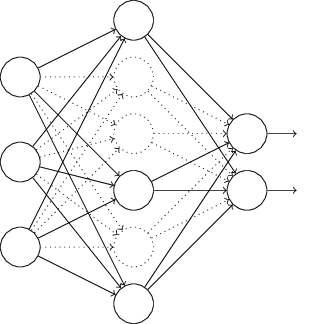
\includegraphics[width=0.45\linewidth]{figures/ch3/tikz31}
\end{center}
We forward-propagate the input $x$ through the modified network, and then backpropagate the result, also through the modified network. After doing this over a mini-batch of examples, we update the appropriate weights and biases. We then repeat the process, first restoring the dropout neurons, then choosing a new random subset of hidden neurons to delete, estimating the gradient for a different mini-batch, and updating the weights and biases in the network.

By repeating this process over and over, our network will learn a set of weights and biases. Of course, those weights and biases will have been learnt under conditions in which half the hidden neurons were dropped out. When we actually run the full network that means that twice as many hidden neurons will be active. To compensate for that, we halve the weights outgoing from the hidden neurons.

This dropout procedure may seem strange and \textit{ad hoc}. Why would we expect it to help with regularization? To explain what's going on, I'd like you to briefly stop thinking about dropout, and instead imagine training neural networks in the standard way (no dropout). In particular, imagine we train several different neural networks, all using the same training data. Of course, the networks may not start out identical, and as a result after training they may sometimes give different results. When that happens we could use some kind of averaging or voting scheme to decide which output to accept. For instance, if we have trained five networks, and three of them are classifying a digit as a ``3'', then it probably really is a ``3''. The other two networks are probably just making a mistake. This kind of averaging scheme is often found to be a powerful (though expensive) way of reducing overfitting. The reason is that the different networks may overfit in different ways, and averaging may help eliminate that kind of overfitting.

What's this got to do with dropout? Heuristically, when we dropout different sets of neurons, it's rather like we're training different neural networks. And so the dropout procedure is like averaging the effects of a very large number of different networks. The different networks will overfit in different ways, and so, hopefully, the net effect of dropout will be to reduce overfitting.


A related heuristic explanation for dropout is given in one of the earliest papers to use the technique\footnote{\href{https://papers.nips.cc/paper/4824-imagenet-classification-with-deep-convolutional-neural-networks.pdf}{ImageNet Classification with Deep Convolutional Neural Networks}, by Alex Krizhevsky, Ilya Sutskever, and Geoffrey Hinton (2012).}: ``This technique reduces complex co-adaptations of neurons, since a neuron cannot rely on the presence of particular other neurons. It is, therefore, forced to learn more robust features that are useful in conjunction with many different random subsets of the other neurons.'' In other words, if we think of our network as a model which is making predictions, then we can think of dropout as a way of making sure that the model is robust to the loss of any individual piece of evidence. In this, it's somewhat similar to L1 and L2 regularization, which tend to reduce weights, and thus make the network more robust to losing any individual connection in the network.

Of course, the true measure of dropout is that it has been very successful in improving the performance of neural networks. The original paper\footnote{\href{http://arxiv.org/pdf/1207.0580.pdf}{Improving neural networks by preventing co-adaptation of feature detectors} by Geoffrey Hinton, Nitish Srivastava, Alex Krizhevsky, Ilya Sutskever, and Ruslan Salakhutdinov (2012). Note that the paper discusses a number of subtleties that I have glossed over in this brief introduction.} introducing the technique applied it to many different tasks. For us, it's of particular interest that they applied dropout to MNIST digit classification, using a vanilla feedforward neural network along lines similar to those we've been considering. The paper noted that the best result anyone had achieved up to that point using such an architecture was 98.4 percent classification accuracy on the test set. They improved that to 98.7 percent accuracy using a combination of dropout and a modified form of L2 regularization. Similarly impressive results have been obtained for many other tasks, including problems in image and speech recognition, and natural language processing. Dropout has been especially useful in training large, deep networks, where the problem of overfitting is often acute.

\textbf{Artificially expanding the training data:} We saw earlier that our MNIST classification accuracy dropped down to percentages in the mid-80s when we used only 1,000 training images. It's not surprising that this is the case, since less training data means our network will be exposed to fewer variations in the way human beings write digits. Let's try training our 30 hidden neuron network with a variety of different training data set sizes, to see how performance varies. We train using a mini-batch size of 10, a learning rate $\eta=0.5$, a regularization parameter $\lambda=5.0$, and the cross-entropy cost function. We will train for 30 epochs when the full training data set is used, and scale up the number of epochs proportionally when smaller training sets are used. To ensure the weight decay factor remains the same across training sets, we will use a regularization parameter of $\lambda=5.0$ when the full training data set is used, and scale down $\lambda$ proportionally when smaller training sets are used\footnote{This and the next two graph are produced with the program \inline{more_data.py}.}.
\begin{center}
	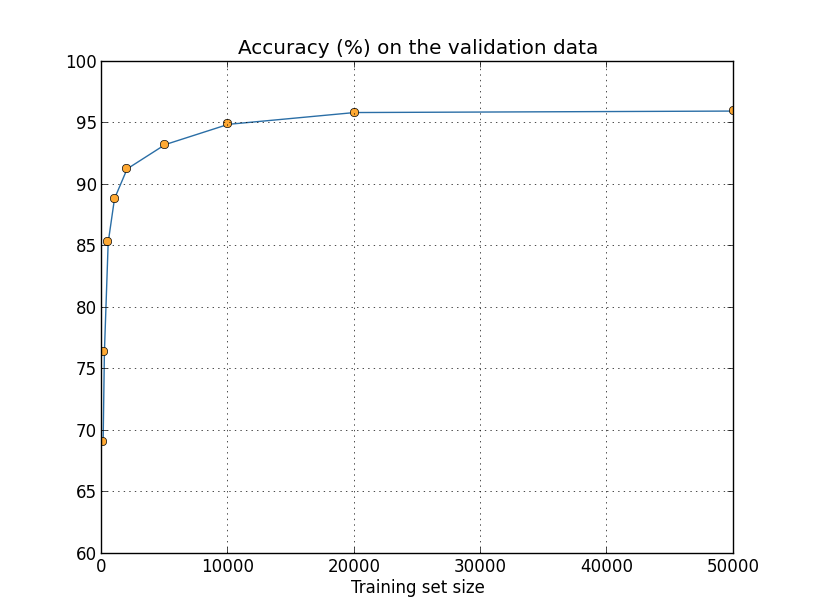
\includegraphics[width=0.6\linewidth]{figures/ch3/more_data}
\end{center}
As you can see, the classification accuracies improve considerably as we use more training data. Presumably this improvement would continue still further if more data was available. Of course, looking at the graph above it does appear that we're getting near saturation. Suppose, however, that we redo the graph with the training set size plotted logarithmically:
\begin{center}
	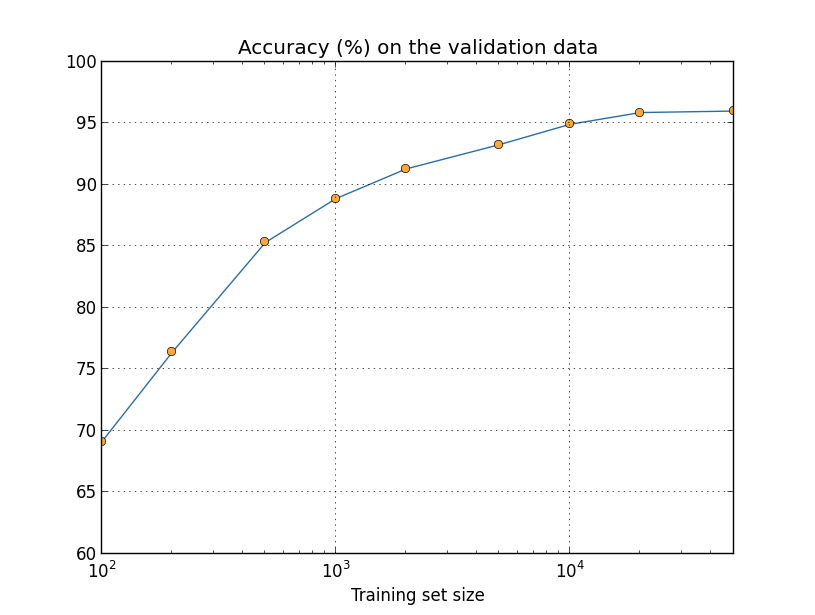
\includegraphics[width=0.6\linewidth]{figures/ch3/more_data_log}
\end{center}
It seems clear that the graph is still going up toward the end. This suggests that if we used vastly more training data -- say, millions or even billions of handwriting samples, instead of just 50,000 -- then we'd likely get considerably better performance, even from this very small network.

Obtaining more training data is a great idea. Unfortunately, it can be expensive, and so is not always possible in practice. However, there's another idea which can work nearly as well, and that's to artificially expand the training data. Suppose, for example, that we take an MNIST training image of a five,
\begin{center}
	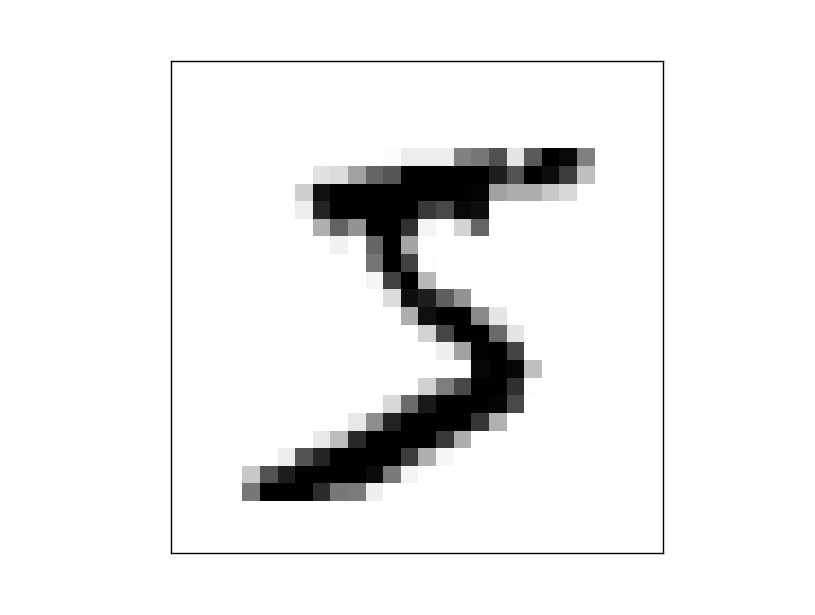
\includegraphics[width=0.15\linewidth]{figures/ch3/more_data_5}
\end{center}
and rotate it by a small amount, let's say 15 degrees:
\begin{center}
	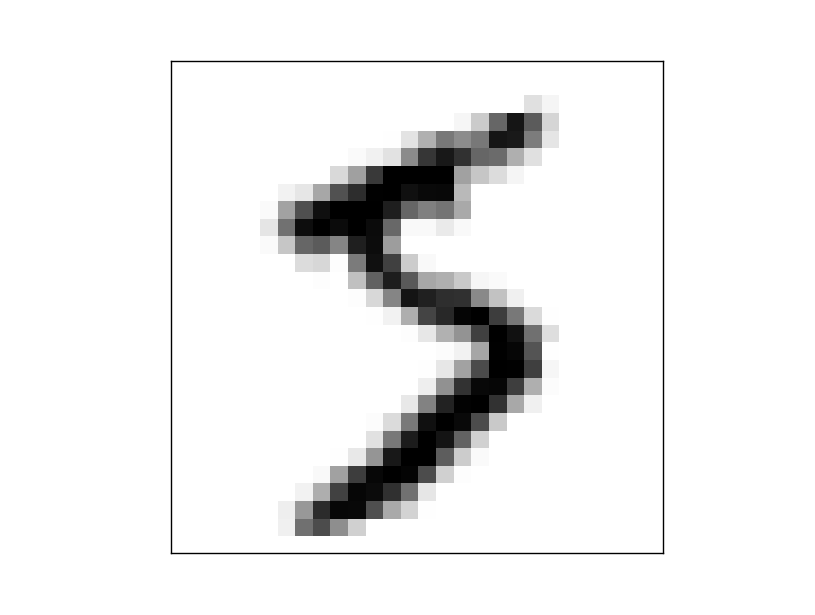
\includegraphics[width=0.15\linewidth]{figures/ch3/more_data_rotated_5}
\end{center}
It's still recognizably the same digit. And yet at the pixel level it's quite different to any image currently in the MNIST training data. It's conceivable that adding this image to the training data might help our network learn more about how to classify digits. What's more, obviously we're not limited to adding just this one image. We can expand our training data by making \textit{many} small rotations of \textit{all} the MNIST training images, and then using the expanded training data to improve our network's performance.

This idea is very powerful and has been widely used. Let's look at some of the results from a paper\footnote{\href{http://dx.doi.org/10.1109/ICDAR.2003.1227801}{Best Practices for Convolutional Neural Networks Applied to Visual Document Analysis} by Patrice Simard, Dave Steinkraus, and John Platt (2003).} which applied several variations of the idea to MNIST. One of the neural network architectures they considered was along similar lines to what we've been using, a feedforward network with 800 hidden neurons and using the cross-entropy cost function. Running the network with the standard MNIST training data they achieved a classification accuracy of 98.4 percent on their test set. But then they expanded the training data, using not just rotations, as I described above, but also translating and skewing the images. By training on the expanded data set they increased their network's accuracy to 98.9 percent. They also experimented with what they called ``elastic distortions'', a special type of image distortion intended to emulate the random oscillations found in hand muscles. By using the elastic distortions to expand the data they achieved an even higher accuracy, 99.3 percent. Effectively, they were broadening the experience of their network by exposing it to the sort of variations that are found in real handwriting.

Variations on this idea can be used to improve performance on many learning tasks, not just handwriting recognition. The general principle is to expand the training data by applying operations that reflect real-world variation. It's not difficult to think of ways of doing this. Suppose, for example, that you're building a neural network to do speech recognition. We humans can recognize speech even in the presence of distortions such as background noise. And so you can expand your data by adding background noise. We can also recognize speech if it's sped up or slowed down. So that's another way we can expand the training data. These techniques are not always used -- for instance, instead of expanding the training data by adding noise, it may well be more efficient to clean up the input to the network by first applying a noise reduction filter. Still, it's worth keeping the idea of expanding the training data in mind, and looking for opportunities to apply it.


\begin{exercize}{Exercise}
	\item As discussed above, one way of expanding the MNIST training data is to use small rotations of training images. What's a problem that might occur if we allow arbitrarily large rotations of training images?
\end{exercize}
\textbf{An aside on big data and what it means to compare classification accuracies:} Let's look again at how our neural network's accuracy varies with training set size:
\begin{center}
	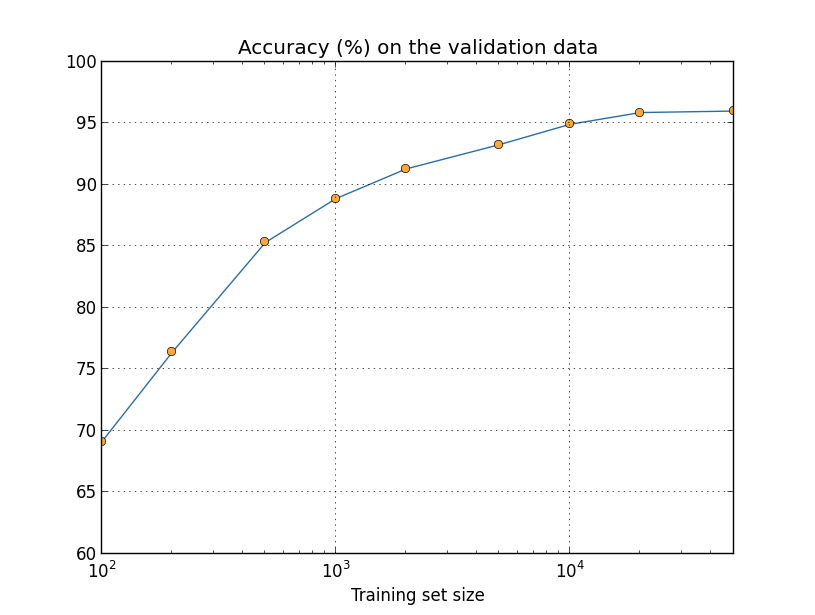
\includegraphics[width=0.6\linewidth]{figures/ch3/more_data_log}
\end{center}
Suppose that instead of using a neural network we use some other machine learning technique to classify digits. For instance, let's try using the support vector machines (SVM) which we met briefly back in Chapter 1. As was the case in Chapter 1, don't worry if you're not familiar with SVMs, we don't need to understand their details. Instead, we'll use the SVM supplied by the scikit-learn library. Here's how SVM performance varies as a function of training set size. I've plotted the neural net results as well, to make comparison easy\footnote{This graph was produced with the program \inline{more_data.py} (as were the last few graphs).}:
\begin{center}
	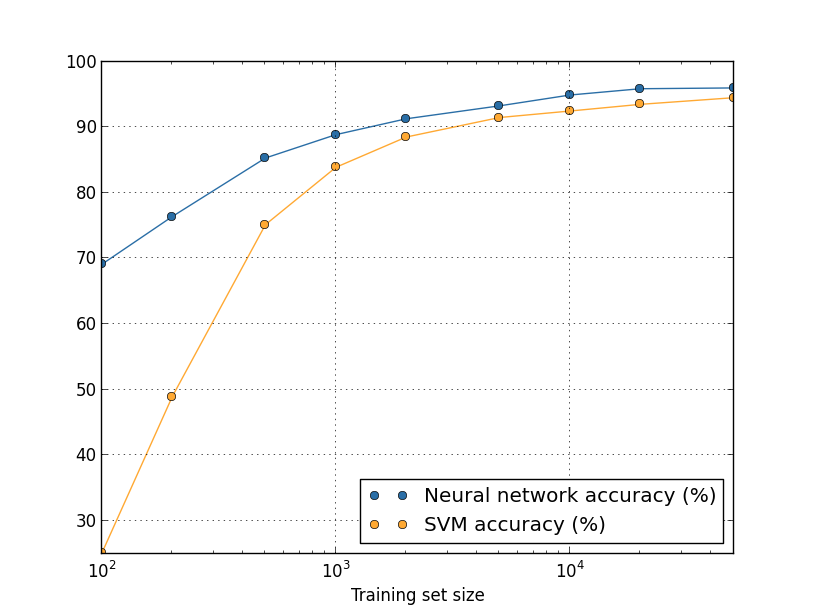
\includegraphics[width=0.6\linewidth]{figures/ch3/more_data_comparison}
\end{center}
Probably the first thing that strikes you about this graph is that our neural network outperforms the SVM for every training set size. That's nice, although you shouldn't read too much into it, since I just used the out-of-the-box settings from scikit-learn's SVM, while we've done a fair bit of work improving our neural network. A more subtle but more interesting fact about the graph is that if we train our SVM using 50,000 images then it actually has better performance (94.48 percent accuracy) than our neural network does when trained using 5,000 images (93.24 percent accuracy). In other words, more training data can sometimes compensate for differences in the machine learning algorithm used.

Something even more interesting can occur. Suppose we're trying to solve a problem using two machine learning algorithms, algorithm A and algorithm B. It sometimes happens that algorithm A will outperform algorithm B with one set of training data, while algorithm B will outperform algorithm A with a different set of training data. We don't see that above -- it would require the two graphs to cross -- but it does happen\footnote{Striking examples may be found in \href{http://dx.doi.org/10.3115/1073012.1073017}{Scaling to very very large corpora for natural language disambiguation}, by Michele Banko and Eric Brill (2001).}. The correct response to the question ``Is algorithm A better than algorithm B?'' is really: ``What training data set are you using?''

All this is a caution to keep in mind, both when doing development, and when reading research papers. Many papers focus on finding new tricks to wring out improved performance on standard benchmark data sets. ``Our whiz-bang technique gave us an improvement of X percent on standard benchmark Y'' is a canonical form of research claim. Such claims are often genuinely interesting, but they must be understood as applying only in the context of the specific training data set used. Imagine an alternate history in which the people who originally created the benchmark data set had a larger research grant. They might have used the extra money to collect more training data. It's entirely possible that the ``improvement'' due to the whiz-bang technique would disappear on a larger data set. In other words, the purported improvement might be just an accident of history. The message to take away, especially in practical applications, is that what we want is both better algorithms and better training data. It's fine to look for better algorithms, but make sure you're not focusing on better algorithms to the exclusion of easy wins getting more or better training data.


\begin{exercize}{Problem}
	\item \textbf{(Research problem)} How do our machine learning algorithms perform in the limit of very large data sets? For any given algorithm it's natural to attempt to define a notion of asymptotic performance in the limit of truly big data. A quick-and-dirty approach to this problem is to simply try fitting curves to graphs like those shown above, and then to extrapolate the fitted curves out to infinity. An objection to this approach is that different approaches to curve fitting will give different notions of asymptotic performance. Can you find a principled justification for fitting to some particular class of curves? If so, compare the asymptotic performance of several different machine learning algorithms.
\end{exercize}
\textbf{Summing up:} We've now completed our dive into overfitting and regularization. Of course, we'll return again to the issue. As I've mentioned several times, overfitting is a major problem in neural networks, especially as computers get more powerful, and we have the ability to train larger networks. As a result there's a pressing need to develop powerful regularization techniques to reduce overfitting, and this is an extremely active area of current work.

\section{Weight initialization}
\label{sec:3.3}
When we create our neural networks, we have to make choices for the initial weights and biases. Up to now, we've been choosing them according to a prescription which I discussed only briefly back in Chapter 1. Just to remind you, that prescription was to choose both the weights and biases using independent Gaussian random variables, normalized to have mean 0 and standard deviation 1. While this approach has worked well, it was quite ad hoc, and it's worth revisiting to see if we can find a better way of setting our initial weights and biases, and perhaps help our neural networks learn faster.

It turns out that we can do quite a bit better than initializing with normalized Gaussians. To see why, suppose we're working with a network with a large number -- say 1,000 -- of input neurons. And let's suppose we've used normalized Gaussians to initialize the weights connecting to the first hidden layer. For now I'm going to concentrate specifically on the weights connecting the input neurons to the first neuron in the hidden layer, and ignore the rest of the network:
\begin{center}
	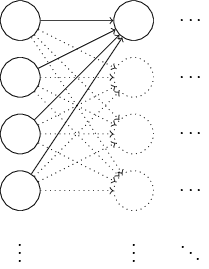
\includegraphics[width=0.35\linewidth]{figures/ch3/tikz32}
\end{center}
We'll suppose for simplicity that we're trying to train using a training input $x$ in which half the input neurons are on, i.e., set to 1, and half the input neurons are off, i.e., set to 0. The argument which follows applies more generally, but you'll get the gist from this special case. Let's consider the weighted sum $z=\sum_jw_jx_j+b$ of inputs to our hidden neuron. 500 terms in this sum vanish, because the corresponding input $x_j$ is zero. And so $z$ is a sum over a total of 501 normalized Gaussian random variables, accounting for the 500 weight terms and the 1 extra bias term. Thus $z$ is itself distributed as a Gaussian with mean zero and standard deviation $\sqrt{501}\approx 22.4$. That is, $z$ has a very broad Gaussian distribution, not sharply peaked at all:
\begin{center}
\begin{tikzpicture}
\begin{axis}[axis lines=middle,width=0.9\linewidth,height=0.35\linewidth,ymin=0,ymax=0.022,ytick={0,0.01,0.02},scaled y ticks = false,y tick label style={/pgf/number format/fixed},xmin=-32,xmax=32]
\addplot[blue,domain=-30:30,samples=81]{exp(-x^2/2/501)/sqrt(2*pi*501)};
\end{axis}
\end{tikzpicture}
\end{center}
In particular, we can see from this graph that it's quite likely that $|z|$ will be pretty large, i.e., either $z\gg1$ or $z\ll-1$. If that's the case then the output $\sigma(z)$ from the hidden neuron will be very close to either 1 or 0. That means our hidden neuron will have saturated. And when that happens, as we know, making small changes in the weights will make only absolutely miniscule changes in the activation of our hidden neuron. That miniscule change in the activation of the hidden neuron will, in turn, barely affect the rest of the neurons in the network at all, and we'll see a correspondingly miniscule change in the cost function. As a result, those weights will only learn very slowly when we use the gradient descent algorithm\footnote{We discussed this in more detail in Chapter 2, where we used the equations of backpropagation to show that weights input to saturated neurons learned slowly.}. It's similar to the problem we discussed earlier in this chapter, in which output neurons which saturated on the wrong value caused learning to slow down. We addressed that earlier problem with a clever choice of cost function. Unfortunately, while that helped with saturated output neurons, it does nothing at all for the problem with saturated hidden neurons.

I've been talking about the weights input to the first hidden layer. Of course, similar arguments apply also to later hidden layers: if the weights in later hidden layers are initialized using normalized Gaussians, then activations will often be very close to 0 or 1, and learning will proceed very slowly.

Is there some way we can choose better initializations for the weights and biases, so that we don't get this kind of saturation, and so avoid a learning slowdown? Suppose we have a neuron with $n_\mathrm{in}$ input weights. Then we shall initialize those weights as Gaussian random variables with mean 0 and standard deviation $1/\sqrt{n_\mathrm{in}}$. That is, we'll squash the Gaussians down, making it less likely that our neuron will saturate. We'll continue to choose the bias as a Gaussian with mean 0 and standard deviation 1, for reasons I'll return to in a moment. With these choices, the weighted sum $z=\sum_jw_jx_j+b$ will again be a Gaussian random variable with mean 0, but it'll be much more sharply peaked than it was before. Suppose, as we did earlier, that 500 of the inputs are zero and 500 are 1. Then it's easy to show (see the exercise below) that $z$ has a Gaussian distribution with mean 0 and standard deviation $\sqrt{3/2}=1.22\ldots$. This is much more sharply peaked than before, so much so that even the graph below understates the situation, since I've had to rescale the vertical axis, when compared to the earlier graph:
\begin{center}
\begin{tikzpicture}
\begin{axis}[axis lines=middle,width=0.9\linewidth,height=0.35\linewidth,ymin=0,ymax=0.45,ytick={0,0.4},scaled y ticks = false,y tick label style={/pgf/number format/fixed},xmin=-32,xmax=32]
\addplot[blue,domain=-10:10,samples=201]{exp(-x^2/2/1.5)/sqrt(2*pi*1.5)};
\end{axis}
\end{tikzpicture}
\end{center}
Such a neuron is much less likely to saturate, and correspondingly much less likely to have problems with a learning slowdown.

\begin{exercize}{Exercise}
	\item Verify that the standard deviation of $z=\sum_jw_jx_j+b$ in the paragraph above is $\sqrt{3/2}$. It may help to know that: (a)~the variance of a sum of independent random variables is the sum of the variances of the individual random variables; and (b)~the variance is the square of the standard deviation.
\end{exercize}
I stated above that we'll continue to initialize the biases as before, as Gaussian random variables with a mean of 0 and a standard deviation of 1. This is okay, because it doesn't make it too much more likely that our neurons will saturate. In fact, it doesn't much matter how we initialize the biases, provided we avoid the problem with saturation. Some people go so far as to initialize all the biases to 0, and rely on gradient descent to learn appropriate biases. But since it's unlikely to make much difference, we'll continue with the same initialization procedure as before.

Let's compare the results for both our old and new approaches to weight initialization, using the MNIST digit classification task. As before, we'll use 30 hidden neurons, a mini-batch size of 10, a regularization parameter $\lambda=5.0$, and the cross-entropy cost function. We will decrease the learning rate slightly from $\eta=0.5$ to 0.1, since that makes the results a little more easily visible in the graphs. We can train using the old method of weight initialization:
\begin{lstlisting}
>>> import mnist_loader
>>> training_data, validation_data, test_data =  mnist_loader.load_data_wrapper()
>>> import network2
>>> net = network2.Network([784, 30, 10], cost=network2.CrossEntropyCost)
>>> net.large_weight_initializer()
>>> net.SGD(training_data, 30, 10, 0.1, lmbda = 5.0,  evaluation_data=validation_data, 
... monitor_evaluation_accuracy=True)
\end{lstlisting}
We can also train using the new approach to weight initialization. This is actually even easier, since network2's default way of initializing the weights is using this new approach. That means we can omit the \inline{net.large_weight_initializer()} call above: 
\begin{lstlisting}
>>> net = network2.Network([784, 30, 10], cost=network2.CrossEntropyCost)
>>> net.SGD(training_data, 30, 10, 0.1, lmbda = 5.0, evaluation_data=validation_data, 
... monitor_evaluation_accuracy=True)
\end{lstlisting}
Plotting the results\footnote{The program used to generate this and the next graph is \inline{weight_initialization.py}.}, we obtain:
\begin{center}
	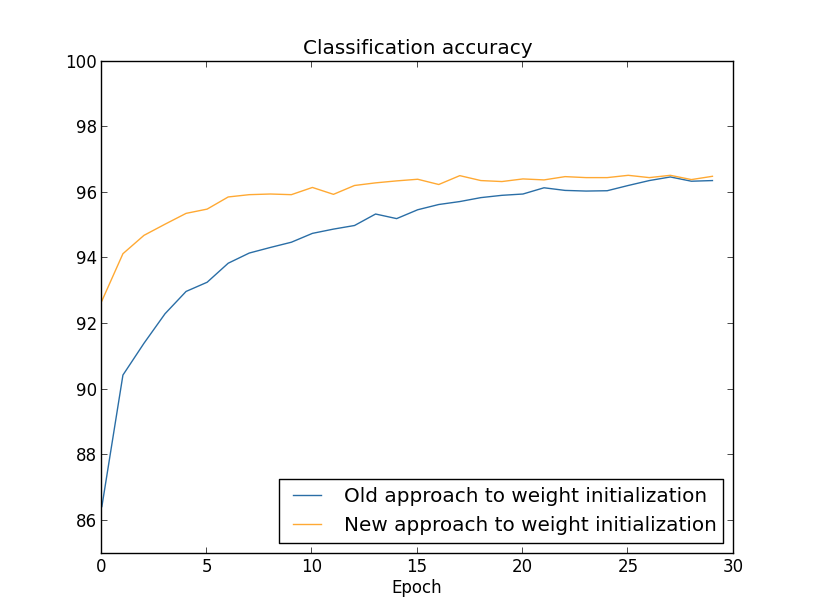
\includegraphics[width=0.6\linewidth]{figures/ch3/weight_initialization_30}
\end{center}
In both cases, we end up with a classification accuracy somewhat over 96 percent. The final classification accuracy is almost exactly the same in the two cases. But the new initialization technique brings us there much, much faster. At the end of the first epoch of training the old approach to weight initialization has a classification accuracy under 87 percent, while the new approach is already almost 93 percent. What appears to be going on is that our new approach to weight initialization starts us off in a much better regime, which lets us get good results much more quickly. The same phenomenon is also seen if we plot results with 100 hidden neurons:
\begin{center}
	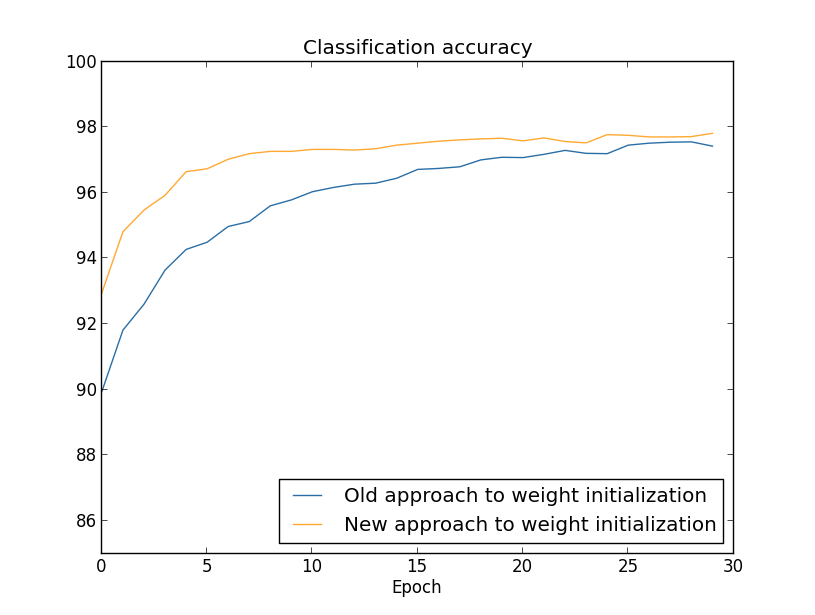
\includegraphics[width=0.6\linewidth]{figures/ch3/weight_initialization_100}
\end{center}
In this case, the two curves don't quite meet. However, my experiments suggest that with just a few more epochs of training (not shown) the accuracies become almost exactly the same. So on the basis of these experiments it looks as though the improved weight initialization only speeds up learning, it doesn't change the final performance of our networks. However, in Chapter 4 we'll see examples of neural networks where the long-run behaviour is significantly better with the $1/\sqrt{n_{\rm in}}$ weight initialization. Thus it's not only the speed of learning which is improved, it's sometimes also the final performance.

The $1/\sqrt{n_{\rm in}}$ approach to weight initialization helps improve the way our neural nets learn. Other techniques for weight initialization have also been proposed, many building on this basic idea. I won't review the other approaches here, since $1/\sqrt{n_{\rm in}}$ works well enough for our purposes. If you're interested in looking further, I recommend looking at the discussion on pages 14 and 15 of a 2012 paper by Yoshua Bengio\footnote{\href{http://arxiv.org/pdf/1206.5533v2.pdf}{Practical Recommendations for Gradient-Based Training of Deep Architectures}, by Yoshua Bengio (2012).}, as well as the references therein.

\begin{exercize}{Problem}
	\item \textbf{Connecting regularization and the improved method of weight initialization} L2 regularization sometimes automatically gives us something similar to the new approach to weight initialization. Suppose we are using the old approach to weight initialization. Sketch a heuristic argument that: (1) supposing $\lambda$ is not too small, the first epochs of training will be dominated almost entirely by weight decay; (2) provided $\eta\lambda\ll n$ the weights will decay by a factor of $\exp(-\eta\lambda/m)$ per epoch; and (3) supposing $\lambda$ is not too large, the weight decay will tail off when the weights are down to a size around $1/\sqrt{n_{\rm in}}$, where $n$ is the total number of weights in the network. Argue that these conditions are all satisfied in the examples graphed in this section.
	\end{exercize}

\section{Handwriting recognition revisited: the code}
\label{sec:3.4}
Let's implement the ideas we've discussed in this chapter. We'll develop a new program, \inline{network2.py}, which is an improved version of the program \inline{network.py} we developed in Chapter 1. If you haven't looked at \inline{network.py} in a while then you may find it helpful to spend a few minutes quickly reading over the earlier discussion. It's only 74 lines of code, and is easily understood.

As was the case in \inline{network.py}, the star of \inline{network2.py} is the \inline{Network} class, which we use to represent our neural networks. We initialize an instance of \inline{Network} with a list of \inline{sizes} for the respective layers in the network, and a choice for the cost to use, defaulting to the cross-entropy:
\begin{lstlisting}
class Network(object):
	def __init__(self, sizes, cost=CrossEntropyCost):
		self.num_layers = len(sizes)
		self.sizes = sizes
		self.default_weight_initializer()
		self.cost=cost
\end{lstlisting}
The first couple of lines of the \inline{__init__} method are the same as in \inline{network.py}, and are pretty self-explanatory. But the next two lines are new, and we need to understand what they're doing in detail.

Let's start by examining the \inline{default_weight_initializer} method. This makes use of our new and improved approach to weight initialization. As we've seen, in that approach the weights input to a neuron are initialized as Gaussian random variables with mean 0 and standard deviation 1 divided by the square root of the number of connections input to the neuron. Also in this method we'll initialize the biases, using Gaussian random variables with mean 0 and standard deviation 1. Here's the code:
\begin{lstlisting}
def default_weight_initializer(self):
	self.biases = [np.random.randn(y, 1) for y in self.sizes[1:]]
	self.weights = [np.random.randn(y, x)/np.sqrt(x) for x, y in zip(self.sizes[:-1], self.sizes[1:])]
\end{lstlisting}
To understand the code, it may help to recall that \inline{np} is the Numpy library for doing linear algebra. We'll import Numpy at the beginning of our program. Also, notice that we don't initialize any biases for the first layer of neurons. We avoid doing this because the first layer is an input layer, and so any biases would not be used. We did exactly the same thing in \inline{network.py}.

Complementing the \inline{default_weight_initializer} we'll also include a \texttt{large\_weight\_initializer} method. This method initializes the weights and biases using the old approach from Chapter 1, with both weights and biases initialized as Gaussian random variables with mean 0 and standard deviation 1. The code is, of course, only a tiny bit different from the \inline{default_weight_initializer}:
\begin{lstlisting}
def large_weight_initializer(self):
	self.biases = [np.random.randn(y, 1) for y in self.sizes[1:]]
	self.weights = [np.random.randn(y, x) for x, y in zip(self.sizes[:-1], self.sizes[1:])]
\end{lstlisting}
	
I've included the \inline{large_weight_initializer} method mostly as a convenience to make it easier to compare the results in this chapter to those in Chapter 1. I can't think of many practical situations where I would recommend using it!

The second new thing in \inline{Network}'s \inline{__init__} method is that we now initialize a cost attribute. To understand how that works, let's look at the class we use to represent the cross-entropy cost\footnote{If you're not familiar with Python's static methods you can ignore the \inline{@staticmethod} decorators, and just treat \inline{fn} and \inline{delta} as ordinary methods. If you're curious about details, all \inline{@staticmethod} does is tell the Python interpreter that the method which follows doesn't depend on the object in any way. That's why self isn't passed as a parameter to the \inline{fn} and \inline{delta} methods.}:
\begin{lstlisting} 
class CrossEntropyCost(object):
	@staticmethod
	def fn(a, y):
		return np.sum(np.nan_to_num(-y*np.log(a)-(1-y)*np.log(1-a)))
	@staticmethod
	def delta(z, a, y):
		return (a-y)
\end{lstlisting}
Let's break this down. The first thing to observe is that even though the cross-entropy is, mathematically speaking, a function, we've implemented it as a Python class, not a Python function. Why have I made that choice? The reason is that the cost plays two different roles in our network. The obvious role is that it's a measure of how well an output activation, \inline{a}, matches the desired output, \inline{y}. This role is captured by the \inline{CrossEntropyCost.fn} method. (Note, by the way, that the \inline{np.nan_to_num} call inside \inline{CrossEntropyCost.fn} ensures that Numpy deals correctly with the log of numbers very close to zero.) But there's also a second way the cost function enters our network. Recall from Chapter 2 that when running the backpropagation algorithm we need to compute the network's output error, $\delta^L$. The form of the output error depends on the choice of cost function: different cost function, different form for the output error. For the cross-entropy the output error is, as we saw in Equation (\ref{eq:66}),
\begin{equation}
	\delta^L=a^L-y.\label{eq:99}
\end{equation}
%δL=aL-y.(99)
For this reason we define a second method, \inline{CrossEntropyCost.delta}, whose purpose is to tell our network how to compute the output error. And then we bundle these two methods up into a single class containing everything our networks need to know about the cost function.

In a similar way, \inline{network2.py} also contains a class to represent the quadratic cost function. This is included for comparison with the results of Chapter 1, since going forward we'll mostly use the cross entropy. The code is just below. The \inline{QuadraticCost.fn} method is a straightforward computation of the quadratic cost associated to the actual output, \inline{a}, and the desired output, \inline{y}. The value returned by \inline{QuadraticCost.delta} is based on the expression (\ref{eq:30}) for the output error for the quadratic cost, which we derived back in Chapter 2.

\begin{lstlisting}
class QuadraticCost(object):
	@staticmethod
	def fn(a, y):
		return 0.5*np.linalg.norm(a-y)**2
	@staticmethod
	def delta(z, a, y):
		return (a-y) * sigmoid_prime(z)
\end{lstlisting}
We've now understood the main differences between \inline{network2.py} and \inline{network.py}. It's all pretty simple stuff. There are a number of smaller changes, which I'll discuss below, including the implementation of L2 regularization. Before getting to that, let's look at the complete code for \inline{network2.py}. You don't need to read all the code in detail, but it is worth understanding the broad structure, and in particular reading the documentation strings, so you understand what each piece of the program is doing. Of course, you're also welcome to delve as deeply as you wish! If you get lost, you may wish to continue reading the prose below, and return to the code later. Anyway, here's the code:
\begin{lstlisting}
"""network2.py
~~~~~~~~~~~~~~

An improved version of network.py, implementing the stochastic
gradient descent learning algorithm for a feedforward neural network.
Improvements include the addition of the cross-entropy cost function,
regularization, and better initialization of network weights.  Note
that I have focused on making the code simple, easily readable, and
easily modifiable.  It is not optimized, and omits many desirable
features.
"""
#### Libraries
# Standard library
import json
import random
import sys
# Third-party libraries
import numpy as np

#### Define the quadratic and cross-entropy cost functions

class QuadraticCost(object):

	@staticmethod
	def fn(a, y):
		"""Return the cost associated with an output ``a`` and desired output	``y``.
		"""
		return 0.5*np.linalg.norm(a-y)**2

	@staticmethod
	def delta(z, a, y):
		"""Return the error delta from the output layer."""
		return (a-y) * sigmoid_prime(z)

class CrossEntropyCost(object):

	@staticmethod
		def fn(a, y):
		"""Return the cost associated with an output ``a`` and desired output
		``y``.  Note that np.nan_to_num is used to ensure numerical
		stability.  In particular, if both ``a`` and ``y`` have a 1.0
		in the same slot, then the expression (1-y)*np.log(1-a)
		returns nan.  The np.nan_to_num ensures that that is converted
		to the correct value (0.0).
		
		"""
		return np.sum(np.nan_to_num(-y*np.log(a)-(1-y)*np.log(1-a)))

	@staticmethod
	def delta(z, a, y):
		"""Return the error delta from the output layer.  Note that the
		parameter ``z`` is not used by the method.  It is included in
		the method's parameters in order to make the interface
		consistent with the delta method for other cost classes.
		
		"""
		return (a-y)


#### Main Network class
class Network(object):
	
	def __init__(self, sizes, cost=CrossEntropyCost):
		"""The list ``sizes`` contains the number of neurons in the respective
		layers of the network.  For example, if the list was [2, 3, 1]
		then it would be a three-layer network, with the first layer
		containing 2 neurons, the second layer 3 neurons, and the
		third layer 1 neuron.  The biases and weights for the network
		are initialized randomly, using
		``self.default_weight_initializer`` (see docstring for that
		method).
		
		"""
		self.num_layers = len(sizes)
		self.sizes = sizes
		self.default_weight_initializer()
		self.cost=cost

	def default_weight_initializer(self):
		"""Initialize each weight using a Gaussian distribution with mean 0
		and standard deviation 1 over the square root of the number of
		weights connecting to the same neuron.  Initialize the biases
		using a Gaussian distribution with mean 0 and standard
		deviation 1.
	
		Note that the first layer is assumed to be an input layer, and
		by convention we won't set any biases for those neurons, since
		biases are only ever used in computing the outputs from later
		layers.
		
		"""
		self.biases = [np.random.randn(y, 1) for y in self.sizes[1:]]
		self.weights = [np.random.randn(y, x)/np.sqrt(x) for x, y in zip(self.sizes[:-1], self.sizes[1:])]

	def large_weight_initializer(self):
		"""Initialize the weights using a Gaussian distribution with mean 0
		and standard deviation 1.  Initialize the biases using a
		Gaussian distribution with mean 0 and standard deviation 1.
		
		Note that the first layer is assumed to be an input layer, and
		by convention we won't set any biases for those neurons, since
		biases are only ever used in computing the outputs from later
		layers.
		
		This weight and bias initializer uses the same approach as in
		Chapter 1, and is included for purposes of comparison.  It
		will usually be better to use the default weight initializer
		instead.
		
		"""
		self.biases = [np.random.randn(y, 1) for y in self.sizes[1:]]
		self.weights = [np.random.randn(y, x)
		for x, y in zip(self.sizes[:-1], self.sizes[1:])]
	
	def feedforward(self, a):
		"""Return the output of the network if ``a`` is input."""
		for b, w in zip(self.biases, self.weights):
		a = sigmoid(np.dot(w, a)+b)
		return a
	
	def SGD(self, training_data, epochs, mini_batch_size, eta, lmbda = 0.0, evaluation_data=None, monitor_evaluation_cost=False, monitor_evaluation_accuracy=False, monitor_training_cost=False, monitor_training_accuracy=False):
		"""Train the neural network using mini-batch stochastic gradient
		descent.  The ``training_data`` is a list of tuples ``(x, y)``
		representing the training inputs and the desired outputs.  The
		other non-optional parameters are self-explanatory, as is the
		regularization parameter ``lmbda``.  The method also accepts
		``evaluation_data``, usually either the validation or test
		data.  We can monitor the cost and accuracy on either the
		evaluation data or the training data, by setting the
		appropriate flags.  The method returns a tuple containing four
		lists: the (per-epoch) costs on the evaluation data, the
		accuracies on the evaluation data, the costs on the training
		data, and the accuracies on the training data.  All values are
		evaluated at the end of each training epoch.  So, for example,
		if we train for 30 epochs, then the first element of the tuple
		will be a 30-element list containing the cost on the
		evaluation data at the end of each epoch. Note that the lists
		are empty if the corresponding flag is not set.
		
		"""
		if evaluation_data:
			n_data = len(evaluation_data)
		n = len(training_data)
		evaluation_cost, evaluation_accuracy = [], []
		training_cost, training_accuracy = [], []
		for j in xrange(epochs):
			random.shuffle(training_data)
			mini_batches = [
				training_data[k:k+mini_batch_size]
				for k in xrange(0, n, mini_batch_size)]
			for mini_batch in mini_batches:
				self.update_mini_batch(
					mini_batch, eta, lmbda, len(training_data))
			print "Epoch %s training complete" % j
			if monitor_training_cost:
				cost = self.total_cost(training_data, lmbda)
				training_cost.append(cost)
				print "Cost on training data: {}".format(cost)
			if monitor_training_accuracy:
				accuracy = self.accuracy(training_data, convert=True)
				training_accuracy.append(accuracy)
				print "Accuracy on training data: {} / {}".format(accuracy, n)
			if monitor_evaluation_cost:
				cost = self.total_cost(evaluation_data, lmbda, convert=True)
				evaluation_cost.append(cost)
				print "Cost on evaluation data: {}".format(cost)
			if monitor_evaluation_accuracy:
				accuracy = self.accuracy(evaluation_data)
				evaluation_accuracy.append(accuracy)
				print "Accuracy on evaluation data: {} / {}".format(self.accuracy(evaluation_data), n_data)
			print
		return evaluation_cost, evaluation_accuracy, training_cost, training_accuracy

	def update_mini_batch(self, mini_batch, eta, lmbda, n):
		"""Update the network's weights and biases by applying gradient
		descent using backpropagation to a single mini batch.  The
		``mini_batch`` is a list of tuples ``(x, y)``, ``eta`` is the
		learning rate, ``lmbda`` is the regularization parameter, and
		``n`` is the total size of the training data set.
		
		"""
		nabla_b = [np.zeros(b.shape) for b in self.biases]
		nabla_w = [np.zeros(w.shape) for w in self.weights]
		for x, y in mini_batch:
			delta_nabla_b, delta_nabla_w = self.backprop(x, y)
			nabla_b = [nb+dnb for nb, dnb in zip(nabla_b, delta_nabla_b)]
			nabla_w = [nw+dnw for nw, dnw in zip(nabla_w, delta_nabla_w)]
		self.weights = [(1-eta*(lmbda/n))*w-(eta/len(mini_batch))*nw
						for w, nw in zip(self.weights, nabla_w)]
		self.biases = [b-(eta/len(mini_batch))*nb
						for b, nb in zip(self.biases, nabla_b)]

	def backprop(self, x, y):
		"""Return a tuple ``(nabla_b, nabla_w)`` representing the
		gradient for the cost function C_x.  ``nabla_b`` and
		``nabla_w`` are layer-by-layer lists of numpy arrays, similar
		to ``self.biases`` and ``self.weights``."""
		nabla_b = [np.zeros(b.shape) for b in self.biases]
		nabla_w = [np.zeros(w.shape) for w in self.weights]
		# feedforward
		activation = x
		activations = [x] # list to store all the activations, layer by layer
		zs = [] # list to store all the z vectors, layer by layer
		for b, w in zip(self.biases, self.weights):
			z = np.dot(w, activation)+b
			zs.append(z)
			activation = sigmoid(z)
			activations.append(activation)
		# backward pass
		delta = (self.cost).delta(zs[-1], activations[-1], y)
		nabla_b[-1] = delta
		nabla_w[-1] = np.dot(delta, activations[-2].transpose())
		# Note that the variable l in the loop below is used a little
		# differently to the notation in Chapter 2 of the book.  Here,
		# l = 1 means the last layer of neurons, l = 2 is the
		# second-last layer, and so on.  It's a renumbering of the
		# scheme in the book, used here to take advantage of the fact
		# that Python can use negative indices in lists.
		for l in xrange(2, self.num_layers):
			z = zs[-l]
			sp = sigmoid_prime(z)
			delta = np.dot(self.weights[-l+1].transpose(), delta) * sp
			nabla_b[-l] = delta
			nabla_w[-l] = np.dot(delta, activations[-l-1].transpose())
		return (nabla_b, nabla_w)
	
	def accuracy(self, data, convert=False):
		"""Return the number of inputs in ``data`` for which the neural
		network outputs the correct result. The neural network's
		output is assumed to be the index of whichever neuron in the
		final layer has the highest activation.
		
		The flag ``convert`` should be set to False if the data set is
		validation or test data (the usual case), and to True if the
		data set is the training data. The need for this flag arises
		due to differences in the way the results ``y`` are
		represented in the different data sets.  In particular, it
		flags whether we need to convert between the different
		representations.  It may seem strange to use different
		representations for the different data sets.  Why not use the
		same representation for all three data sets?  It's done for
		efficiency reasons -- the program usually evaluates the cost
		on the training data and the accuracy on other data sets.
		These are different types of computations, and using different
		representations speeds things up.  More details on the
		representations can be found in
		mnist_loader.load_data_wrapper.
		
		"""
		if convert:
			results = [(np.argmax(self.feedforward(x)), np.argmax(y)) for (x, y) in data]
		else:
			results = [(np.argmax(self.feedforward(x)), y)	for (x, y) in data]
		return sum(int(x == y) for (x, y) in results)
	
	def total_cost(self, data, lmbda, convert=False):
		"""Return the total cost for the data set ``data``.  The flag
		``convert`` should be set to False if the data set is the
		training data (the usual case), and to True if the data set is
		the validation or test data.  See comments on the similar (but
		reversed) convention for the ``accuracy`` method, above.
		"""
		cost = 0.0
		for x, y in data:
			a = self.feedforward(x)
		if convert:
			y = vectorized_result(y)
		cost += self.cost.fn(a, y)/len(data)
		cost += 0.5*(lmbda/len(data))*sum(np.linalg.norm(w)**2 for w in self.weights)
		return cost
	
	def save(self, filename):
		"""Save the neural network to the file ``filename``."""
		data = {"sizes": self.sizes,
			"weights": [w.tolist() for w in self.weights],
			"biases": [b.tolist() for b in self.biases],
			"cost": str(self.cost.__name__)}
		f = open(filename, "w")
		json.dump(data, f)
		f.close()
		
	#### Loading a Network
	def load(filename):
		"""Load a neural network from the file ``filename``.  Returns an
		instance of Network.
		
		"""
		f = open(filename, "r")
		data = json.load(f)
		f.close()
		cost = getattr(sys.modules[__name__], data["cost"])
		net = Network(data["sizes"], cost=cost)
		net.weights = [np.array(w) for w in data["weights"]]
		net.biases = [np.array(b) for b in data["biases"]]
		return net
	
	#### Miscellaneous functions
	def vectorized_result(j):
		"""Return a 10-dimensional unit vector with a 1.0 in the j'th position
		and zeroes elsewhere.  This is used to convert a digit (0...9)
		into a corresponding desired output from the neural network.
		
		"""
		e = np.zeros((10, 1))
		e[j] = 1.0
		return e
	
	def sigmoid(z):
		"""The sigmoid function."""
		return 1.0/(1.0+np.exp(-z))
	
	def sigmoid_prime(z):
		"""Derivative of the sigmoid function."""
		return sigmoid(z)*(1-sigmoid(z))
\end{lstlisting}
One of the more interesting changes in the code is to include L2 regularization. Although this is a major conceptual change, it's so trivial to implement that it's easy to miss in the code. For the most part it just involves passing the parameter \inline{lmbda} to various methods, notably the \inline{Network.SGD} method. The real work is done in a single line of the program, the fourth-last line of the \inline{Network.update_mini_batch} method. That's where we modify the gradient descent update rule to include weight decay. But although the modification is tiny, it has a big impact on results!

This is, by the way, common when implementing new techniques in neural networks. We've spent thousands of words discussing regularization. It's conceptually quite subtle and difficult to understand. And yet it was trivial to add to our program! It occurs surprisingly often that sophisticated techniques can be implemented with small changes to code.

Another small but important change to our code is the addition of several optional flags to the stochastic gradient descent method, Network.SGD. These flags make it possible to monitor the cost and accuracy either on the \inline{training_data} or on a set of \inline{evaluation_data} which can be passed to \inline{Network.SGD}. We've used these flags often earlier in the chapter, but let me give an example of how it works, just to remind you:
\begin{lstlisting}
>>> import mnist_loader
>>> training_data, validation_data, test_data =  mnist_loader.load_data_wrapper()
>>> import network2
>>> net = network2.Network([784, 30, 10], cost=network2.CrossEntropyCost)
>>> net.SGD(training_data, 30, 10, 0.5, lmbda = 5.0, evaluation_data=validation_data,
... monitor_evaluation_accuracy=True, monitor_evaluation_cost=True, monitor_training_accuracy=True,
... monitor_training_cost=True)
\end{lstlisting}
Here, we're setting the \inline{evaluation_data} to be the \inline{validation_data}. But we could also have monitored performance on the \inline{test_data} or any other data set. We also have four flags telling us to monitor the cost and accuracy on both the \inline{evaluation_data} and the \inline{training_data}. Those flags are False by default, but they've been turned on here in order to monitor our \inline{Network}'s performance. Furthermore, \inline{network2.py}'s \inline{Network.SGD} method returns a four-element tuple representing the results of the monitoring. We can use this as follows:
\begin{lstlisting}
>>> evaluation_cost, evaluation_accuracy,  training_cost, training_accuracy = net.SGD(training_data, 30, 10, 0.5,  lmbda = 5.0, evaluation_data=validation_data, monitor_evaluation_accuracy=True, monitor_evaluation_cost=True, monitor_training_accuracy=True, monitor_training_cost=True)
\end{lstlisting}

So, for example, \inline{evaluation_cost} will be a 30-element list containing the cost on the evaluation data at the end of each epoch. This sort of information is extremely useful in understanding a network's behaviour. It can, for example, be used to draw graphs showing how the network learns over time. Indeed, that's exactly how I constructed all the graphs earlier in the chapter. Note, however, that if any of the monitoring flags are not set, then the corresponding element in the tuple will be the empty list.

Other additions to the code include a \inline{Network.save} method, to save \inline{Network} objects to disk, and a function to load them back in again later. Note that the saving and loading is done using JSON, not Python's pickle or cPickle modules, which are the usual way we save and load objects to and from disk in Python. Using JSON requires more code than pickle or cPickle would. To understand why I've used JSON, imagine that at some time in the future we decided to change our \inline{Network} class to allow neurons other than sigmoid neurons. To implement that change we'd most likely change the attributes defined in the \inline{Network.__init__} method. If we've simply pickled the objects that would cause our load function to fail. Using JSON to do the serialization explicitly makes it easy to ensure that old Networks will still load.

There are many other minor changes in the code for \inline{network2.py}, but they're all simple variations on \inline{network.py}. The net result is to expand our 74-line program to a far more capable 152 lines.


\begin{exercize}{Problems}
\item Modify the code above to implement L1 regularization, and use L1 regularization to classify MNIST digits using a 30 hidden neuron network. Can you find a regularization parameter that enables you to do better than running unregularized?
\item Take a look at the \inline{Network.cost_derivative} method in \inline{network.py}. That method was written for the quadratic cost. How would you rewrite the method for the cross-entropy cost? Can you think of a problem that might arise in the cross-entropy version? In \inline{network2.py} we've eliminated the \inline{Network.cost_derivative} method entirely, instead incorporating its functionality into the \inline{CrossEntropyCost.delta} method. How does this solve the problem you've just identified?
\end{exercize}
\section{How to choose a neural network's hyper-parameters?}
\label{sec:3.5}
Up until now I haven't explained how I've been choosing values for hyper-parameters such as the learning rate, $\eta$, the regularization parameter, $\lambda$, and so on. I've just been supplying values which work pretty well. In practice, when you're using neural nets to attack a problem, it can be difficult to find good hyper-parameters. Imagine, for example, that we've just been introduced to the MNIST problem, and have begun working on it, knowing nothing at all about what hyper-parameters to use. Let's suppose that by good fortune in our first experiments we choose many of the hyper-parameters in the same way as was done earlier this chapter: 30 hidden neurons, a mini-batch size of 10, training for 30 epochs using the cross-entropy. But we choose a learning rate $\eta=10.0$ and regularization parameter $\lambda=1000.0$. Here's what I saw on one such run:

\begin{lstlisting}

>>> import mnist_loader
>>> training_data, validation_data, test_data = \
... mnist_loader.load_data_wrapper()
>>> import network2
>>> net = network2.Network([784, 30, 10])
>>> net.SGD(training_data, 30, 10, 10.0, lmbda = 1000.0,
... evaluation_data=validation_data, monitor_evaluation_accuracy=True)


Epoch 0 training complete
Accuracy on evaluation data: 1030 / 10000

Epoch 1 training complete
Accuracy on evaluation data: 990 / 10000

Epoch 2 training complete
Accuracy on evaluation data: 1009 / 10000

...

Epoch 27 training complete
Accuracy on evaluation data: 1009 / 10000

Epoch 28 training complete
Accuracy on evaluation data: 983 / 10000

Epoch 29 training complete
Accuracy on evaluation data: 967 / 10000
\end{lstlisting}
Our classification accuracies are no better than chance! Our network is acting as a random noise generator!

``Well, that's easy to fix,'' you might say, ``just decrease the learning rate and regularization hyper-parameters''. Unfortunately, you don't a priori know those are the hyper-parameters you need to adjust. Maybe the real problem is that our 30 hidden neuron network will never work well, no matter how the other hyper-parameters are chosen? Maybe we really need at least 100 hidden neurons? Or 300 hidden neurons? Or multiple hidden layers? Or a different approach to encoding the output? Maybe our network is learning, but we need to train for more epochs? Maybe the mini-batches are too small? Maybe we'd do better switching back to the quadratic cost function? Maybe we need to try a different approach to weight initialization? And so on, on and on and on. It's easy to feel lost in hyper-parameter space. This can be particularly frustrating if your network is very large, or uses a lot of training data, since you may train for hours or days or weeks, only to get no result. If the situation persists, it damages your confidence. Maybe neural networks are the wrong approach to your problem? Maybe you should quit your job and take up beekeeping?

In this section I explain some heuristics which can be used to set the hyper-parameters in a neural network. The goal is to help you develop a workflow that enables you to do a pretty good job setting hyper-parameters. Of course, I won't cover everything about hyper-parameter optimization. That's a huge subject, and it's not, in any case, a problem that is ever completely solved, nor is there universal agreement amongst practitioners on the right strategies to use. There's always one more trick you can try to eke out a bit more performance from your network. But the heuristics in this section should get you started.

\textbf{Broad strategy:} When using neural networks to attack a new problem the first challenge is to get any non-trivial learning, i.e., for the network to achieve results better than chance. This can be surprisingly difficult, especially when confronting a new class of problem. Let's look at some strategies you can use if you're having this kind of trouble.

Suppose, for example, that you're attacking MNIST for the first time. You start out enthusiastic, but are a little discouraged when your first network fails completely, as in the example above. The way to go is to strip the problem down. Get rid of all the training and validation images except images which are 0s or 1s. Then try to train a network to distinguish 0s from 1s. Not only is that an inherently easier problem than distinguishing all ten digits, it also reduces the amount of training data by 80 percent, speeding up training by a factor of 5. That enables much more rapid experimentation, and so gives you more rapid insight into how to build a good network.

You can further speed up experimentation by stripping your network down to the simplest network likely to do meaningful learning. If you believe a \inline{[784, 10]} network can likely do better-than-chance classification of MNIST digits, then begin your experimentation with such a network. It'll be much faster than training a \inline{[784, 30, 10]} network, and you can build back up to the latter.

You can get another speed up in experimentation by increasing the frequency of monitoring. In \inline{network2.py} we monitor performance at the end of each training epoch. With 50,000 images per epoch, that means waiting a little while -- about ten seconds per epoch, on my laptop, when training a [784, 30, 10] network -- before getting feedback on how well the network is learning. Of course, ten seconds isn't very long, but if you want to trial dozens of hyper-parameter choices it's annoying, and if you want to trial hundreds or thousands of choices it starts to get debilitating. We can get feedback more quickly by monitoring the validation accuracy more often, say, after every 1,000 training images. Furthermore, instead of using the full 10,000 image validation set to monitor performance, we can get a much faster estimate using just 100 validation images. All that matters is that the network sees enough images to do real learning, and to get a pretty good rough estimate of performance. Of course, our program \inline{network2.py} doesn't currently do this kind of monitoring. But as a kludge to achieve a similar effect for the purposes of illustration, we'll strip down our training data to just the first 1,000 MNIST training images. Let's try it and see what happens. (To keep the code below simple I haven't implemented the idea of using only 0 and 1 images. Of course, that can be done with just a little more work.)
\begin{lstlisting}
>>> net = network2.Network([784, 10])
>>> net.SGD(training_data[:1000], 30, 10, 10.0, lmbda = 1000.0, \
... evaluation_data=validation_data[:100], \
... monitor_evaluation_accuracy=True)
Epoch 0 training complete
Accuracy on evaluation data: 10 / 100

Epoch 1 training complete
Accuracy on evaluation data: 10 / 100

Epoch 2 training complete
Accuracy on evaluation data: 10 / 100
...
\end{lstlisting}
We're still getting pure noise! But there's a big win: we're now getting feedback in a fraction of a second, rather than once every ten seconds or so. That means you can more quickly experiment with other choices of hyper-parameter, or even conduct experiments trialling many different choices of hyper-parameter nearly simultaneously.

In the above example I left $\lambda$ as $\lambda=1000.0$, as we used earlier. But since we changed the number of training examples we should really change $\lambda$ to keep the weight decay the same. That means changing $\lambda$ to 20.0. If we do that then this is what happens:
\begin{lstlisting}
>>> net = network2.Network([784, 10])
>>> net.SGD(training_data[:1000], 30, 10, 10.0, lmbda = 20.0, \
... evaluation_data=validation_data[:100], \
... monitor_evaluation_accuracy=True)
Epoch 0 training complete
Accuracy on evaluation data: 12 / 100

Epoch 1 training complete
Accuracy on evaluation data: 14 / 100

Epoch 2 training complete
Accuracy on evaluation data: 25 / 100

Epoch 3 training complete
Accuracy on evaluation data: 18 / 100
...
\end{lstlisting}
Ahah! We have a signal. Not a terribly good signal, but a signal nonetheless. That's something we can build on, modifying the hyper-parameters to try to get further improvement. Maybe we guess that our learning rate needs to be higher. (As you perhaps realize, that's a silly guess, for reasons we'll discuss shortly, but please bear with me.) So to test our guess we try dialing $\eta$ up to 100.0:

\begin{lstlisting}
>>> net = network2.Network([784, 10])
>>> net.SGD(training_data[:1000], 30, 10, 100.0, lmbda = 20.0, \
... evaluation_data=validation_data[:100], \
... monitor_evaluation_accuracy=True)
Epoch 0 training complete
Accuracy on evaluation data: 10 / 100

Epoch 1 training complete
Accuracy on evaluation data: 10 / 100

Epoch 2 training complete
Accuracy on evaluation data: 10 / 100

Epoch 3 training complete
Accuracy on evaluation data: 10 / 100
...
\end{lstlisting}
That's no good! It suggests that our guess was wrong, and the problem wasn't that the learning rate was too low. So instead we try dialing $\eta$ down to $\eta=1.0$:

\begin{lstlisting}
>>> net = network2.Network([784, 10])
>>> net.SGD(training_data[:1000], 30, 10, 1.0, lmbda = 20.0, \
... evaluation_data=validation_data[:100], \
... monitor_evaluation_accuracy=True)
Epoch 0 training complete
Accuracy on evaluation data: 62 / 100

Epoch 1 training complete
Accuracy on evaluation data: 42 / 100

Epoch 2 training complete
Accuracy on evaluation data: 43 / 100

Epoch 3 training complete
Accuracy on evaluation data: 61 / 100
...

\end{lstlisting}
That's better! And so we can continue, individually adjusting each hyper-parameter, gradually improving performance. Once we've explored to find an improved value for $\eta$, then we move on to find a good value for $\lambda$. Then experiment with a more complex architecture, say a network with 10 hidden neurons. Then adjust the values for $\eta$ and $\lambda$ again. Then increase to 20 hidden neurons. And then adjust other hyper-parameters some more. And so on, at each stage evaluating performance using our held-out validation data, and using those evaluations to find better and better hyper-parameters. As we do so, it typically takes longer to witness the impact due to modifications of the hyper-parameters, and so we can gradually decrease the frequency of monitoring.

This all looks very promising as a broad strategy. However, I want to return to that initial stage of finding hyper-parameters that enable a network to learn anything at all. In fact, even the above discussion conveys too positive an outlook. It can be immensely frustrating to work with a network that's learning nothing. You can tweak hyper-parameters for days, and still get no meaningful response. And so I'd like to re-emphasize that during the early stages you should make sure you can get quick feedback from experiments. Intuitively, it may seem as though simplifying the problem and the architecture will merely slow you down. In fact, it speeds things up, since you much more quickly find a network with a meaningful signal. Once you've got such a signal, you can often get rapid improvements by tweaking the hyper-parameters. As with many things in life, getting started can be the hardest thing to do.

Okay, that's the broad strategy. Let's now look at some specific recommendations for setting hyper-parameters. I will focus on the learning rate, $\eta$, the L2 regularization parameter, $\lambda$, and the mini-batch size. However, many of the remarks apply also to other hyper-parameters, including those associated to network architecture, other forms of regularization, and some hyper-parameters we'll meet later in the book, such as the momentum co-efficient.

Learning rate: Suppose we run three MNIST networks with three different learning rates, $\eta=0.025$, $\eta=0.25$ and $\eta=2.5$, respectively. We'll set the other hyper-parameters as for the experiments in earlier sections, running over 30 epochs, with a mini-batch size of 10, and with $\lambda=5.0$. We'll also return to using the full 50,000 training images. Here's a graph showing the behaviour of the training cost as we train\footnote{The graph was generated by \inline{multiple_eta.py}.}:
\begin{center}
	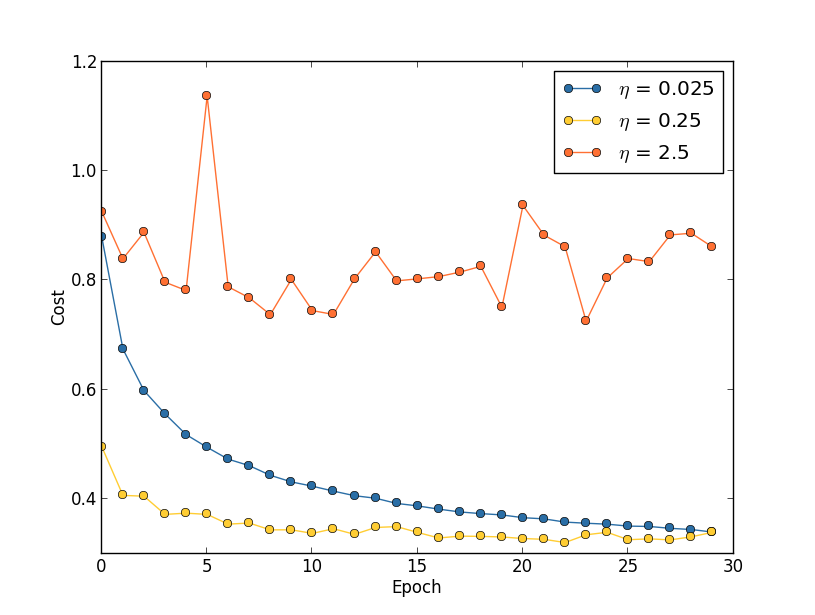
\includegraphics[width=0.7\linewidth]{figures/ch3/multiple_eta}
\end{center}
With $\eta=0.025$ the cost decreases smoothly until the final epoch. With $\eta=0.25$ the cost initially decreases, but after about 20 epochs it is near saturation, and thereafter most of the changes are merely small and apparently random oscillations. Finally, with $\eta=2.5$ the cost makes large oscillations right from the start. To understand the reason for the oscillations, recall that stochastic gradient descent is supposed to step us gradually down into a valley of the cost function,
\begin{center}
	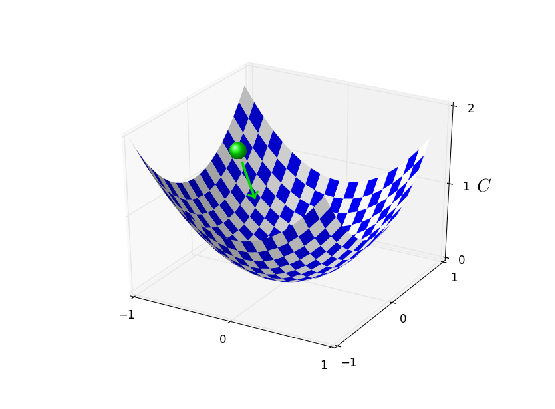
\includegraphics[width=0.5\linewidth]{figures/ch3/tikz33}
\end{center}
However, if $\eta$ is too large then the steps will be so large that they may actually overshoot the minimum, causing the algorithm to climb up out of the valley instead. That's likely* *This picture is helpful, but it's intended as an intuition-building illustration of what may go on, not as a complete, exhaustive explanation. Briefly, a more complete explanation is as follows: gradient descent uses a first-order approximation to the cost function as a guide to how to decrease the cost. For large $\eta$, higher-order terms in the cost function become more important, and may dominate the behaviour, causing gradient descent to break down. This is especially likely as we approach minima and quasi-minima of the cost function, since near such points the gradient becomes small, making it easier for higher-order terms to dominate behaviour. what's causing the cost to oscillate when $\eta=2.5$. When we choose $\eta$=0.25 the initial steps do take us toward a minimum of the cost function, and it's only once we get near that minimum that we start to suffer from the overshooting problem. And when we choose $\eta=0.025$ we don't suffer from this problem at all during the first 30 epochs. Of course, choosing $\eta$ so small creates another problem, namely, that it slows down stochastic gradient descent. An even better approach would be to start with $\eta=0.25$, train for 20 epochs, and then switch to $\eta=0.025$. We'll discuss such variable learning rate schedules later. For now, though, let's stick to figuring out how to find a single good value for the learning rate, $\eta$.

With this picture in mind, we can set $\eta$ as follows. First, we estimate the threshold value for $\eta$ at which the cost on the training data immediately begins decreasing, instead of oscillating or increasing. This estimate doesn't need to be too accurate. You can estimate the order of magnitude by starting with $\eta$=0.01. If the cost decreases during the first few epochs, then you should successively try $\eta=0.1,1.0,\ldots$ until you find a value for $\eta$ where the cost oscillates or increases during the first few epochs. Alternately, if the cost oscillates or increases during the first few epochs when $\eta$=0.01, then try $\eta$=0.001,0.0001,$\ldots$ until you find a value for $\eta$ where the cost decreases during the first few epochs. Following this procedure will give us an order of magnitude estimate for the threshold value of $\eta$. You may optionally refine your estimate, to pick out the largest value of $\eta$ at which the cost decreases during the first few epochs, say $\eta$=0.5 or $\eta$=0.2 (there's no need for this to be super-accurate). This gives us an estimate for the threshold value of $\eta$.

Obviously, the actual value of $\eta$ that you use should be no larger than the threshold value. In fact, if the value of $\eta$ is to remain usable over many epochs then you likely want to use a value for $\eta$ that is smaller, say, a factor of two below the threshold. Such a choice will typically allow you to train for many epochs, without causing too much of a slowdown in learning.

In the case of the MNIST data, following this strategy leads to an estimate of 0.1 for the order of magnitude of the threshold value of $\eta$. After some more refinement, we obtain a threshold value $\eta$=0.5. Following the prescription above, this suggests using $\eta$=0.25 as our value for the learning rate. In fact, I found that using $\eta$=0.5 worked well enough over 30 epochs that for the most part I didn't worry about using a lower value of $\eta$.

This all seems quite straightforward. However, using the training cost to pick $\eta$ appears to contradict what I said earlier in this section, namely, that we'd pick hyper-parameters by evaluating performance using our held-out validation data. In fact, we'll use validation accuracy to pick the regularization hyper-parameter, the mini-batch size, and network parameters such as the number of layers and hidden neurons, and so on. Why do things differently for the learning rate? Frankly, this choice is my personal aesthetic preference, and is perhaps somewhat idiosyncratic. The reasoning is that the other hyper-parameters are intended to improve the final classification accuracy on the test set, and so it makes sense to select them on the basis of validation accuracy. However, the learning rate is only incidentally meant to impact the final classification accuracy. Its primary purpose is really to control the step size in gradient descent, and monitoring the training cost is the best way to detect if the step size is too big. With that said, this is a personal aesthetic preference. Early on during learning the training cost usually only decreases if the validation accuracy improves, and so in practice it's unlikely to make much difference which criterion you use.


\textbf{Use early stopping to determine the number of training epochs:} As we discussed earlier in the chapter, early stopping means that at the end of each epoch we should compute the classification accuracy on the validation data. When that stops improving, terminate. This makes setting the number of epochs very simple. In particular, it means that we don't need to worry about explicitly figuring out how the number of epochs depends on the other hyper-parameters. Instead, that's taken care of automatically. Furthermore, early stopping also automatically prevents us from overfitting. This is, of course, a good thing, although in the early stages of experimentation it can be helpful to turn off early stopping, so you can see any signs of overfitting, and use it to inform your approach to regularization.

To implement early stopping we need to say more precisely what it means that the classification accuracy has stopped improving. As we've seen, the accuracy can jump around quite a bit, even when the overall trend is to improve. If we stop the first time the accuracy decreases then we'll almost certainly stop when there are more improvements to be had. A better rule is to terminate if the best classification accuracy doesn't improve for quite some time. Suppose, for example, that we're doing MNIST. Then we might elect to terminate if the classification accuracy hasn't improved during the last ten epochs. This ensures that we don't stop too soon, in response to bad luck in training, but also that we're not waiting around forever for an improvement that never comes.

This no-improvement-in-ten rule is good for initial exploration of MNIST. However, networks can sometimes plateau near a particular classification accuracy for quite some time, only to then begin improving again. If you're trying to get really good performance, the no-improvement-in-ten rule may be too aggressive about stopping. In that case, I suggest using the no-improvement-in-ten rule for initial experimentation, and gradually adopting more lenient rules, as you better understand the way your network trains: no-improvement-in-twenty, no-improvement-in-fifty, and so on. Of course, this introduces a new hyper-parameter to optimize! In practice, however, it's usually easy to set this hyper-parameter to get pretty good results. Similarly, for problems other than MNIST, the no-improvement-in-ten rule may be much too aggressive or not nearly aggressive enough, depending on the details of the problem. However, with a little experimentation it's usually easy to find a pretty good strategy for early stopping.

We haven't used early stopping in our MNIST experiments to date. The reason is that we've been doing a lot of comparisons between different approaches to learning. For such comparisons it's helpful to use the same number of epochs in each case. However, it's well worth modifying \inline{network2.py} to implement early stopping:

\begin{exercize}{Problem}
\item Modify \inline{network2.py} so that it implements early stopping using a no-improvement-in-$n$ epochs strategy, where $n$ is a parameter that can be set.
\item Can you think of a rule for early stopping other than no-improvement-in-$n$? Ideally, the rule should compromise between getting high validation accuracies and not training too long. Add your rule to \inline{network2.py}, and run three experiments comparing the validation accuracies and number of epochs of training to no-improvement-in-10.
\end{exercize}
\textbf{Learning rate schedule:} We've been holding the learning rate $\eta$ constant. However, it's often advantageous to vary the learning rate. Early on during the learning process it's likely that the weights are badly wrong. And so it's best to use a large learning rate that causes the weights to change quickly. Later, we can reduce the learning rate as we make more fine-tuned adjustments to our weights.

How should we set our learning rate schedule? Many approaches are possible. One natural approach is to use the same basic idea as early stopping. The idea is to hold the learning rate constant until the validation accuracy starts to get worse. Then decrease the learning rate by some amount, say a factor of two or ten. We repeat this many times, until, say, the learning rate is a factor of 1,024 (or 1,000) times lower than the initial value. Then we terminate.

A variable learning schedule can improve performance, but it also opens up a world of possible choices for the learning schedule. Those choices can be a headache -- you can spend forever trying to optimize your learning schedule. For first experiments my suggestion is to use a single, constant value for the learning rate. That'll get you a good first approximation. Later, if you want to obtain the best performance from your network, it's worth experimenting with a learning schedule, along the lines I've described\footnote{A readable recent paper which demonstrates the benefits of variable learning rates in attacking MNIST is \href{http://arxiv.org/abs/1003.0358}{Deep, Big, Simple Neural Nets Excel on Handwritten Digit Recognition}, by Dan Claudiu Cire\c{s}an, Ueli Meier, Luca Maria Gambardella, and J\"urgen Schmidhuber (2010).}.

\begin{exercize}{Exercise}
	\item Modify \inline{network2.py} so that it implements a learning schedule that: halves the learning rate each time the validation accuracy satisfies the no-improvement-in-10 rule; and terminates when the learning rate has dropped to 1/128 of its original value.
\end{exercize}
\textbf{The regularization parameter,} $\lambda$: I suggest starting initially with no regularization ($\lambda=0.0$), and determining a value for $\eta$, as above. Using that choice of $\eta$, we can then use the validation data to select a good value for $\lambda$. Start by trialling $\lambda=1.0$\footnote{I don't have a good principled justification for using this as a starting value. If anyone knows of a good principled discussion of where to start with $\lambda$, I'd appreciate hearing it (mn@michaelnielsen.org).}, and then increase or decrease by factors of 10, as needed to improve performance on the validation data. Once you've found a good order of magnitude, you can fine tune your value of $\lambda$. That done, you should return and re-optimize $\eta$ again.

\begin{exercize}{Exercise}
\item It's tempting to use gradient descent to try to learn good values for hyper-parameters such as $\lambda$ and $\eta$. Can you think of an obstacle to using gradient descent to determine $\lambda$? Can you think of an obstacle to using gradient descent to determine $\eta$?
\end{exercize}
\textbf{How I selected hyper-parameters earlier in this book:} If you use the recommendations in this section you'll find that you get values for $\eta$ and $\lambda$ which don't always exactly match the values I've used earlier in the book. The reason is that the book has narrative constraints that have sometimes made it impractical to optimize the hyper-parameters. Think of all the comparisons we've made of different approaches to learning, e.g., comparing the quadratic and cross-entropy cost functions, comparing the old and new methods of weight initialization, running with and without regularization, and so on. To make such comparisons meaningful, I've usually tried to keep hyper-parameters constant across the approaches being compared (or to scale them in an appropriate way). Of course, there's no reason for the same hyper-parameters to be optimal for all the different approaches to learning, so the hyper-parameters I've used are something of a compromise.

As an alternative to this compromise, I could have tried to optimize the heck out of the hyper-parameters for every single approach to learning. In principle that'd be a better, fairer approach, since then we'd see the best from every approach to learning. However, we've made dozens of comparisons along these lines, and in practice I found it too computationally expensive. That's why I've adopted the compromise of using pretty good (but not necessarily optimal) choices for the hyper-parameters.


\textbf{Mini-batch size:} How should we set the mini-batch size? To answer this question, let's first suppose that we're doing online learning, i.e., that we're using a mini-batch size of 1.

The obvious worry about online learning is that using mini-batches which contain just a single training example will cause significant errors in our estimate of the gradient. In fact, though, the errors turn out to not be such a problem. The reason is that the individual gradient estimates don't need to be super-accurate. All we need is an estimate accurate enough that our cost function tends to keep decreasing. It's as though you are trying to get to the North Magnetic Pole, but have a wonky compass that's 10--20 degrees off each time you look at it. Provided you stop to check the compass frequently, and the compass gets the direction right on average, you'll end up at the North Magnetic Pole just fine.

Based on this argument, it sounds as though we should use online learning. In fact, the situation turns out to be more complicated than that. In a problem in the last chapter\ref{backprop_over_minibatch} I pointed out that it's possible to use matrix techniques to compute the gradient update for all examples in a mini-batch simultaneously, rather than looping over them. Depending on the details of your hardware and linear algebra library this can make it quite a bit faster to compute the gradient estimate for a mini-batch of (for example) size 100, rather than computing the mini-batch gradient estimate by looping over the 100 training examples separately. It might take (say) only 50 times as long, rather than 100 times as long.

Now, at first it seems as though this doesn't help us that much. With our mini-batch of size 100 the learning rule for the weights looks like:
%w→w′=w-\eta1100∑x∇Cx,(100)
\begin{eqnarray}
w \to w' = w-\eta \frac{1}{100} \sum_x \nabla C_x,
\label{eq:100}\end{eqnarray}
where the sum is over training examples in the mini-batch. This is versus
\begin{eqnarray}
w \rightarrow w' = w-\eta \nabla C_x
\label{eq:101}\end{eqnarray}
%w→w′=w-\eta∇Cx(101)
for online learning. Even if it only takes 50 times as long to do the mini-batch update, it still seems likely to be better to do online learning, because we'd be updating so much more frequently. Suppose, however, that in the mini-batch case we increase the learning rate by a factor 100, so the update rule becomes
%w→w′=w-\eta∑x∇Cx.(102)
\begin{eqnarray}
w \rightarrow w' = w-\eta \sum_x \nabla C_x.
\label{eq:102}\end{eqnarray}
That's a lot like doing 100 separate instances of online learning with a learning rate of $\eta$. But it only takes 50 times as long as doing a single instance of online learning. Of course, it's not truly the same as 100 instances of online learning, since in the mini-batch the $\nabla C_x$'s are all evaluated for the same set of weights, as opposed to the cumulative learning that occurs in the online case. Still, it seems distinctly possible that using the larger mini-batch would speed things up.

With these factors in mind, choosing the best mini-batch size is a compromise. Too small, and you don't get to take full advantage of the benefits of good matrix libraries optimized for fast hardware. Too large and you're simply not updating your weights often enough. What you need is to choose a compromise value which maximizes the speed of learning. Fortunately, the choice of mini-batch size at which the speed is maximized is relatively independent of the other hyper-parameters (apart from the overall architecture), so you don't need to have optimized those hyper-parameters in order to find a good mini-batch size. The way to go is therefore to use some acceptable (but not necessarily optimal) values for the other hyper-parameters, and then trial a number of different mini-batch sizes, scaling $\eta$ as above. Plot the validation accuracy versus time (as in, real elapsed time, not epoch!), and choose whichever mini-batch size gives you the most rapid improvement in performance. With the mini-batch size chosen you can then proceed to optimize the other hyper-parameters.

Of course, as you've no doubt realized, I haven't done this optimization in our work. Indeed, our implementation doesn't use the faster approach to mini-batch updates at all. I've simply used a mini-batch size of 10 without comment or explanation in nearly all examples. Because of this, we could have sped up learning by reducing the mini-batch size. I haven't done this, in part because I wanted to illustrate the use of mini-batches beyond size 1, and in part because my preliminary experiments suggested the speedup would be rather modest. In practical implementations, however, we would most certainly implement the faster approach to mini-batch updates, and then make an effort to optimize the mini-batch size, in order to maximize our overall speed.

\textbf{Automated techniques:} I've been describing these heuristics as though you're optimizing your hyper-parameters by hand. Hand-optimization is a good way to build up a feel for how neural networks behave. However, and unsurprisingly, a great deal of work has been done on automating the process. A common technique is grid search, which systematically searches through a grid in hyper-parameter space. A review of both the achievements and the limitations of grid search (with suggestions for easily-implemented alternatives) may be found in a 2012 paper\footnote{\href{http://dl.acm.org/citation.cfm?id=2188395}{Random search for hyper-parameter optimization}, by James Bergstra and Yoshua Bengio (2012).} by James Bergstra and Yoshua Bengio. Many more sophisticated approaches have also been proposed. I won't review all that work here, but do want to mention a particularly promising 2012 paper which used a Bayesian approach to automatically optimize hyper-parameters\footnote{\href{http://papers.nips.cc/paper/4522-practical-bayesian-optimization-of-machine-learning-algorithms.pdf}{Practical Bayesian optimization of machine learning algorithms}, by Jasper Snoek, Hugo Larochelle, and Ryan Adams.}. The code from the paper is \href{https://github.com/jaberg/hyperopt}{publicly available}, and has been used with some success by other researchers.

\textbf{Summing up:} Following the rules-of-thumb I've described won't give you the absolute best possible results from your neural network. But it will likely give you a good start and a basis for further improvements. In particular, I've discussed the hyper-parameters largely independently. In practice, there are relationships between the hyper-parameters. You may experiment with $\eta$, feel that you've got it just right, then start to optimize for $\lambda$, only to find that it's messing up your optimization for $\eta$. In practice, it helps to bounce backward and forward, gradually closing in good values. Above all, keep in mind that the heuristics I've described are rules of thumb, not rules cast in stone. You should be on the lookout for signs that things aren't working, and be willing to experiment. In particular, this means carefully monitoring your network's behaviour, especially the validation accuracy.

The difficulty of choosing hyper-parameters is exacerbated by the fact that the lore about how to choose hyper-parameters is widely spread, across many research papers and software programs, and often is only available inside the heads of individual practitioners. There are many, many papers setting out (sometimes contradictory) recommendations for how to proceed. However, there are a few particularly useful papers that synthesize and distill out much of this lore. Yoshua Bengio has a 2012 paper\footnote{\href{http://arxiv.org/abs/1206.5533}{Practical recommendations for gradient-based training of deep architectures}, by Yoshua Bengio (2012).} that gives some practical recommendations for using backpropagation and gradient descent to train neural networks, including deep neural nets. Bengio discusses many issues in much more detail than I have, including how to do more systematic hyper-parameter searches. Another good paper is a 1998 paper\footnote{\href{http://yann.lecun.com/exdb/publis/pdf/lecun-98b.pdf}{Efficient BackProp}, by Yann LeCun, Léon Bottou, Genevieve Orr and Klaus-Robert M\"{u}ller (1998)} by Yann LeCun, L\'{e}on Bottou, Genevieve Orr and Klaus-Robert M\"{u}ller. Both these papers appear in an extremely useful 2012 book that collects many tricks commonly used in neural nets\footnote{\href{http://www.springer.com/computer/theoretical+computer+science/book/978-3-642-35288-1}{Neural Networks: Tricks of the Trade}, edited by Gr\'egoire Montavon, Genevi\`eve Orr, and Klaus-Robert M\"{u}ller.}. The book is expensive, but many of the articles have been placed online by their respective authors with, one presumes, the blessing of the publisher, and may be located using a search engine.

One thing that becomes clear as you read these articles and, especially, as you engage in your own experiments, is that hyper-parameter optimization is not a problem that is ever completely solved. There's always another trick you can try to improve performance. There is a saying common among writers that books are never finished, only abandoned. The same is also true of neural network optimization: the space of hyper-parameters is so large that one never really finishes optimizing, one only abandons the network to posterity. So your goal should be to develop a workflow that enables you to quickly do a pretty good job on the optimization, while leaving you the flexibility to try more detailed optimizations, if that's important.

The challenge of setting hyper-parameters has led some people to complain that neural networks require a lot of work when compared with other machine learning techniques. I've heard many variations on the following complaint: ``Yes, a well-tuned neural network may get the best performance on the problem. On the other hand, I can try a random forest [or SVM or ... insert your own favorite technique] and it just works. I don't have time to figure out just the right neural network.'' Of course, from a practical point of view it's good to have easy-to-apply techniques. This is particularly true when you're just getting started on a problem, and it may not be obvious whether machine learning can help solve the problem at all. On the other hand, if getting optimal performance is important, then you may need to try approaches that require more specialist knowledge. While it would be nice if machine learning were always easy, there is no a priori reason it should be trivially simple.

\section{Other techniques}
\label{sec:3.6}
Each technique developed in this chapter is valuable to know in its own right, but that's not the only reason I've explained them. The larger point is to familiarize you with some of the problems which can occur in neural networks, and with a style of analysis which can help overcome those problems. In a sense, we've been learning how to think about neural nets. Over the remainder of this chapter I briefly sketch a handful of other techniques. These sketches are less in-depth than the earlier discussions, but should convey some feeling for the diversity of techniques available for use in neural networks.

\subsection{Variations on stochastic gradient descent}
\label{sec:3.6.1}
Stochastic gradient descent by backpropagation has served us well in attacking the MNIST digit classification problem. However, there are many other approaches to optimizing the cost function, and sometimes those other approaches offer performance superior to mini-batch stochastic gradient descent. In this section I sketch two such approaches, the Hessian and momentum techniques.

\textbf{Hessian technique:} To begin our discussion it helps to put neural networks aside for a bit. Instead, we're just going to consider the abstract problem of minimizing a cost function $C$ which is a function of many variables, $w=w_1,w_2,\ldots$, so $C=C(w)$. By Taylor's theorem, the cost function can be approximated near a point $w$ by
\begin{eqnarray}
C(w+\Delta w)  =  C(w) + \sum_j \frac{\partial C}{\partial w_j} \Delta w_j + \frac{1}{2} \sum_{jk} \Delta w_j \frac{\partial^2 C}{\partial w_j \partial w_k} \Delta w_k + \ldots
\label{eq:103}
\end{eqnarray}
%C(w+Δw)=C(w)+∑j∂C∂wjΔwj+12∑jkΔwj∂2C∂wj∂wkΔwk+…(103)
We can rewrite this more compactly as
%C(w+Δw)=C(w)+∇C⋅Δw+12ΔwTHΔw+…,(104)
\begin{eqnarray}
C(w+\Delta w) = C(w) + \nabla C \cdot \Delta w + \frac{1}{2} \Delta w^T H \Delta w + \ldots,
\label{eq:104}
\end{eqnarray}
where $\nabla C$ is the usual gradient vector, and $H$ is a matrix known as the \textit{Hessian matrix}, whose $jk$-th entry is $\partial^2C / \partial w_j \partial w_k$. Suppose we approximate $C$ by discarding the higher-order terms represented by $\ldots$ above,
%C(w+Δw)≈C(w)+∇C⋅Δw+12ΔwTHΔw.(105)
\begin{eqnarray} 
C(w+\Delta w) \approx C(w) + \nabla C \cdot \Delta w + \frac{1}{2} \Delta w^T H \Delta w.
\label{eq:105}
\end{eqnarray}
Using calculus we can show that the expression on the right-hand side can be minimized\footnote{Strictly speaking, for this to be a minimum, and not merely an extremum, we need to assume that the Hessian matrix is positive definite. Intuitively, this means that the function $C$ looks like a valley locally, not a mountain or a saddle.} by choosing
\begin{eqnarray}
\Delta w = -H^{-1} \nabla C.
\label{eq:106}
\end{eqnarray}
%Δw=-H-1∇C.(106)
Provided (\ref{eq:105}) is a good approximate expression for the cost function, then we'd expect that moving from the point $w$ to $w+\Delta w = w-H^{-1} \nabla C$ should significantly decrease the cost function. That suggests a possible algorithm for minimizing the cost:
\begin{itemize}
\item Choose a starting point, $w$.
\item Update $w$ to a new point $w' = w-H^{-1} \nabla C$, where the Hessian $H$ and $\nabla C$ are computed at $w$.
\item Update $w'$ to a new point $w''=w'-H'^{-1}\nabla'C$, where the Hessian $H'$ and $\nabla'C$ are computed at $w'$.
\item $\ldots$
\end{itemize}
In practice, (\ref{eq:105}) is only an approximation, and it's better to take smaller steps. We do this by repeatedly changing $w$ by an amount $\Delta w = -\eta H^{-1}\nabla C$, where $\eta$ is known as the learning rate.

This approach to minimizing a cost function is known as the \textit{Hessian technique} or \textit{Hessian optimization}. There are theoretical and empirical results showing that Hessian methods converge on a minimum in fewer steps than standard gradient descent. In particular, by incorporating information about second-order changes in the cost function it's possible for the Hessian approach to avoid many pathologies that can occur in gradient descent. Furthermore, there are versions of the backpropagation algorithm which can be used to compute the Hessian.

If Hessian optimization is so great, why aren't we using it in our neural networks? Unfortunately, while it has many desirable properties, it has one very undesirable property: it's very difficult to apply in practice. Part of the problem is the sheer size of the Hessian matrix. Suppose you have a neural network with $10^7$ weights and biases. Then the corresponding Hessian matrix will contain $10^7\times10^7=10^{14}$ entries. That's a lot of entries! And that makes computing $H^{-1} \nabla C$ extremely difficult in practice. However, that doesn't mean that it's not useful to understand. In fact, there are many variations on gradient descent which are inspired by Hessian optimization, but which avoid the problem with overly-large matrices. Let's take a look at one such technique, momentum-based gradient descent.


\textbf{Momentum-based gradient descent:} Intuitively, the advantage Hessian optimization has is that it incorporates not just information about the gradient, but also information about how the gradient is changing. Momentum-based gradient descent is based on a similar intuition, but avoids large matrices of second derivatives. To understand the momentum technique, think back to our original picture of gradient descent\ref{gradient_descent}, in which we considered a ball rolling down into a valley. At the time, we observed that gradient descent is, despite its name, only loosely similar to a ball falling to the bottom of a valley. The momentum technique modifies gradient descent in two ways that make it more similar to the physical picture. First, it introduces a notion of ``velocity'' for the parameters we're trying to optimize. The gradient acts to change the velocity, not (directly) the ``position'', in much the same way as physical forces change the velocity, and only indirectly affect position. Second, the momentum method introduces a kind of friction term, which tends to gradually reduce the velocity.

Let's give a more precise mathematical description. We introduce velocity variables $v=v_1,v_2,\ldots$, one for each corresponding $w_j$ variable\footnote{In a neural net the $w_j$ variables would, of course, include all weights and biases.}. Then we replace the gradient descent update rule $w \to w'= w-\eta \nabla C$ by
%vw→→v′=\muv-\eta∇Cw′=w+v′.(107)(108)
\begin{align} 
v  \to   v' &=  \mu v - \eta \nabla C \label{eq:107}\\
w  \to  w' &=  w  + v'.\label{eq:108}
\end{align}
In these equations, $\mu$ is a hyper-parameter which controls the amount of damping or friction in the system. To understand the meaning of the equations it's helpful to first consider the case where $\mu=1$, which corresponds to no friction. When that's the case, inspection of the equations shows that the ``force'' $\nabla C$ is now modifying the velocity, $v$, and the velocity is controlling the rate of change of $w$. Intuitively, we build up the velocity by repeatedly adding gradient terms to it. That means that if the gradient is in (roughly) the same direction through several rounds of learning, we can build up quite a bit of steam moving in that direction. Think, for example, of what happens if we're moving straight down a slope:
\begin{center}
	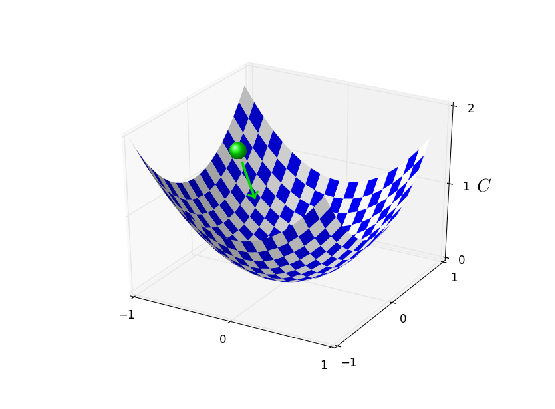
\includegraphics[width=0.55\linewidth]{figures/ch3/tikz34}
\end{center}
With each step the velocity gets larger down the slope, so we move more and more quickly to the bottom of the valley. This can enable the momentum technique to work much faster than standard gradient descent. Of course, a problem is that once we reach the bottom of the valley we will overshoot. Or, if the gradient should change rapidly, then we could find ourselves moving in the wrong direction. That's the reason for the $\mu$ hyper-parameter in (\ref{eq:107}). I said earlier that $\mu$ controls the amount of friction in the system; to be a little more precise, you should think of $1-\mu$ as the amount of friction in the system. When $\mu=1$, as we've seen, there is no friction, and the velocity is completely driven by the gradient $\nabla C$. By contrast, when $\mu=0$ there's a lot of friction, the velocity can't build up, and Equations (\ref{eq:107}) and (\ref{eq:108}) reduce to the usual equation for gradient descent, $w \to w'=w-\eta \nabla C$. In practice, using a value of $\mu$ intermediate between 0 and 1 can give us much of the benefit of being able to build up speed, but without causing overshooting. We can choose such a value for $\mu$ using the held-out validation data, in much the same way as we select $\eta$ and $\lambda$.

I've avoided naming the hyper-parameter $\mu$ up to now. The reason is that the standard name for $\mu$ is badly chosen: it's called the momentum co-efficient. This is potentially confusing, since $\mu$ is not at all the same as the notion of momentum from physics. Rather, it is much more closely related to friction. However, the term momentum co-efficient is widely used, so we will continue to use it.

A nice thing about the momentum technique is that it takes almost no work to modify an implementation of gradient descent to incorporate momentum. We can still use backpropagation to compute the gradients, just as before, and use ideas such as sampling stochastically chosen mini-batches. In this way, we can get some of the advantages of the Hessian technique, using information about how the gradient is changing. But it's done without the disadvantages, and with only minor modifications to our code. In practice, the momentum technique is commonly used, and often speeds up learning.

\begin{exercize}{Exercise}
\item What would go wrong if we used $\mu>1$ in the momentum technique?
\item What would go wrong if we used $\mu<0$ in the momentum technique?
\end{exercize}

\begin{exercize}{Problem}
\item Add momentum-based stochastic gradient descent to \texttt{network2.py}.
\end{exercize}
Other approaches to minimizing the cost function: Many other approaches to minimizing the cost function have been developed, and there isn't universal agreement on which is the best approach. As you go deeper into neural networks it's worth digging into the other techniques, understanding how they work, their strengths and weaknesses, and how to apply them in practice. A paper I mentioned earlier\footnote{\href{http://yann.lecun.com/exdb/publis/pdf/lecun-98b.pdf}{Efficient BackProp}, by Yann LeCun, L\'eon Bottou, Genevieve Orr and Klaus-Robert M\"uller (1998).} introduces and compares several of these techniques, including conjugate gradient descent and the BFGS method (see also the closely related limited-memory BFGS method, known as L-BFGS). Another technique which has recently shown promising results\footnote{See, for example, \href{http://www.cs.toronto.edu/~hinton/absps/momentum.pdf}{On the importance of initialization and momentum in deep learning}, by Ilya Sutskever, James Martens, George Dahl, and Geoffrey Hinton (2012).} is Nesterov's accelerated gradient technique, which improves on the momentum technique. However, for many problems, plain stochastic gradient descent works well, especially if momentum is used, and so we'll stick to stochastic gradient descent through the remainder of this book.

\subsection*{Other models of artificial neuron}
Up to now we've built our neural networks using sigmoid neurons. In principle, a network built from sigmoid neurons can compute any function. In practice, however, networks built using other model neurons sometimes outperform sigmoid networks. Depending on the application, networks based on such alternate models may learn faster, generalize better to test data, or perhaps do both. Let me mention a couple of alternate model neurons, to give you the flavor of some variations in common use.

Perhaps the simplest variation is the tanh (pronounced ``tanch'') neuron, which replaces the sigmoid function by the hyperbolic tangent function. The output of a tanh neuron with input $x$, weight vector $w$, and bias $b$ is given by
\begin{eqnarray}
\tanh(w \cdot x+b), 
\label{eq:109}\end{eqnarray}
%tanh(w⋅x+b),(109)
where $\tanh$ is, of course, the hyperbolic tangent function. It turns out that this is very closely related to the sigmoid neuron. To see this, recall that the tanh function is defined by
\begin{eqnarray}
\tanh(z) \equiv \frac{e^z-e^{-z}}{e^z+e^{-z}}.
\label{eq:110}
\end{eqnarray}
%tanh(z)≡ez-e-zez+e-z.(110)
With a little algebra it can easily be verified that
\begin{eqnarray} 
\sigma(z) = \frac{1+\tanh(z/2)}{2},\label{eq:111}
\end{eqnarray}
%σ(z)=1+tanh(z/2)2,(111)
that is, tanh is just a rescaled version of the sigmoid function. We can also see graphically that the tanh function has the same shape as the sigmoid function,
\begin{center} 
\begin{tikzpicture}
\begin{axis}[title={tanh function},axis lines=middle,width=0.85\linewidth,height=0.5\linewidth,ymin=-1.1,ymax=1.1,scaled y ticks = false,y tick label style={/pgf/number format/fixed},xmin=-5.5,xmax=5.5]
\addplot[thick,blue,domain=-5:5,samples=101]{(exp(x)-exp(-x))/(exp(x)+exp(-x))};
\end{axis}
\end{tikzpicture}
\end{center}
One difference between tanh neurons and sigmoid neurons is that the output from tanh neurons ranges from $-1$ to 1, not 0 to 1. This means that if you're going to build a network based on tanh neurons you may need to normalize your outputs (and, depending on the details of the application, possibly your inputs) a little differently than in sigmoid networks.

Similar to sigmoid neurons, a network of tanh neurons can, in principle, compute any function\footnote{There are some technical caveats to this statement for both tanh and sigmoid neurons, as well as for the rectified linear neurons discussed below. However, informally it's usually fine to think of neural networks as being able to approximate any function to arbitrary accuracy.} mapping inputs to the range $-1$ to 1. Furthermore, ideas such as backpropagation and stochastic gradient descent are as easily applied to a network of tanh neurons as to a network of sigmoid neurons.

\begin{exercize}{Exercise}
	\item Prove the identity in Equation (\ref{eq:111}).
\end{exercize}
Which type of neuron should you use in your networks, the tanh or sigmoid? A priori the answer is not obvious, to put it mildly! However, there are theoretical arguments and some empirical evidence to suggest that the tanh sometimes performs better\footnote{See, for example, \href{http://yann.lecun.com/exdb/publis/pdf/lecun-98b.pdf}{Efficient BackProp}, by Yann LeCun, L\'eon Bottou, Genevieve Orr and Klaus-Robert M\"uller (1998), and \href{http://jmlr.org/proceedings/papers/v9/glorot10a/glorot10a.pdf}{Understanding the difficulty of training deep feedforward networks}, by Xavier Glorot and Yoshua Bengio (2010).}. Let me briefly give you the flavor of one of the theoretical arguments for tanh neurons. Suppose we're using sigmoid neurons, so all activations in our network are positive. Let's consider the weights $w^{l+1}_{jk}$ input to the $j$-th neuron in the $(l+1)$-th layer. The rules for backpropagation  tell us that the associated gradient will be $a^l_k\delta^{l+1}_{j}$. Because the activations are positive the sign of this gradient will be the same as the sign of $\delta^{l+1}_{j}$. What this means is that if $\delta^{l+1}_{j}$ is positive then all the weights $w^{l+1}_{jk}$ will decrease during gradient descent, while if $\delta^{l+1}_{j}$ is negative then all the weights $w^{l+1}_{jk}$ will increase during gradient descent. In other words, all weights to the same neuron must either increase together or decrease together. That's a problem, since some of the weights may need to increase while others need to decrease. That can only happen if some of the input activations have different signs. That suggests replacing the sigmoid by an activation function, such as tanh, which allows both positive and negative activations. Indeed, because tanh is symmetric about zero, $\tanh(-z)=-\tanh(z)$, we might even expect that, roughly speaking, the activations in hidden layers would be equally balanced between positive and negative. That would help ensure that there is no systematic bias for the weight updates to be one way or the other.

How seriously should we take this argument? While the argument is suggestive, it's a heuristic, not a rigorous proof that tanh neurons outperform sigmoid neurons. Perhaps there are other properties of the sigmoid neuron which compensate for this problem? Indeed, for many tasks the tanh is found empirically to provide only a small or no improvement in performance over sigmoid neurons. Unfortunately, we don't yet have hard-and-fast rules to know which neuron types will learn fastest, or give the best generalization performance, for any particular application.

Another variation on the sigmoid neuron is the \textit{rectified linear neuron} or \textit{rectified linear} unit. The output of a rectified linear unit with input $x$, weight vector $w$, and bias $b$ is given by
\begin{eqnarray}
\max(0, w \cdot x+b).
\label{eq:112}
\end{eqnarray}
%max(0,w⋅x+b).(112)
Graphically, the rectifying function $\max(0,z)$ looks like this:
\begin{center} 
	\begin{tikzpicture}
	\begin{axis}[title={$\max(0,z)$},width=0.85\linewidth,height=0.5\linewidth,ymin=-5,ymax=5,scaled y ticks = false,y tick label style={/pgf/number format/fixed},xmin=-5.5,xmax=5.5,axis x line=middle,	axis y line=left, xlabel={$z$}]
	\addplot[thick,blue,domain=-5:5,samples=101]{max(0,x)};
	\end{axis}
	\end{tikzpicture}
\end{center}
Obviously such neurons are quite different from both sigmoid and tanh neurons. However, like the sigmoid and tanh neurons, rectified linear units can be used to compute any function, and they can be trained using ideas such as backpropagation and stochastic gradient descent.

When should you use rectified linear units instead of sigmoid or tanh neurons? Some recent work on image recognition\footnote{See, for example, \href{http://yann.lecun.com/exdb/publis/pdf/jarrett-iccv-09.pdf}{What is the Best Multi-Stage Architecture for Object Recognition?}, by Kevin Jarrett, Koray Kavukcuoglu, Marc'Aurelio Ranzato and Yann LeCun (2009), \href{Deep Sparse Rectifier Neural Networks}, by Xavier Glorot, Antoine Bordes, and Yoshua Bengio (2011), and \href{https://papers.nips.cc/paper/4824-imagenet-classification-with-deep-convolutional-neural-networks.pdf}{ImageNet Classification with Deep Convolutional Neural Networks}, by Alex Krizhevsky, Ilya Sutskever, and Geoffrey Hinton (2012). Note that these papers fill in important details about how to set up the output layer, cost function, and regularization in networks using rectified linear units. I've glossed over all these details in this brief account. The papers also discuss in more detail the benefits and drawbacks of using rectified linear units. Another informative paper is \href{https://www.cs.toronto.edu/~hinton/absps/reluICML.pdf}{Rectified Linear Units Improve Restricted Boltzmann Machines}, by Vinod Nair and Geoffrey Hinton (2010), which demonstrates the benefits of using rectified linear units in a somewhat different approach to neural networks.} has found considerable benefit in using rectified linear units through much of the network. However, as with tanh neurons, we do not yet have a really deep understanding of when, exactly, rectified linear units are preferable, nor why. To give you the flavor of some of the issues, recall that sigmoid neurons stop learning when they saturate, i.e., when their output is near either 0 or 1. As we've seen repeatedly in this chapter, the problem is that $\sigma'$ terms reduce the gradient, and that slows down learning. Tanh neurons suffer from a similar problem when they saturate. By contrast, increasing the weighted input to a rectified linear unit will never cause it to saturate, and so there is no corresponding learning slowdown. On the other hand, when the weighted input to a rectified linear unit is negative, the gradient vanishes, and so the neuron stops learning entirely. These are just two of the many issues that make it non-trivial to understand when and why rectified linear units perform better than sigmoid or tanh neurons.

I've painted a picture of uncertainty here, stressing that we do not yet have a solid theory of how activation functions should be chosen. Indeed, the problem is harder even than I have described, for there are infinitely many possible activation functions. Which is the best for any given problem? Which will result in a network which learns fastest? Which will give the highest test accuracies? I am surprised how little really deep and systematic investigation has been done of these questions. Ideally, we'd have a theory which tells us, in detail, how to choose (and perhaps modify-on-the-fly) our activation functions. On the other hand, we shouldn't let the lack of a full theory stop us! We have powerful tools already at hand, and can make a lot of progress with those tools. Through the remainder of this book I'll continue to use sigmoid neurons as our go-to neuron, since they're powerful and provide concrete illustrations of the core ideas about neural nets. But keep in the back of your mind that these same ideas can be applied to other types of neuron, and that there are sometimes advantages in doing so.

\subsection*{On stories in neural networks}
\begin{adjustwidth}{1.5cm}{1cm}
\textbf{Question:} \textit{How do you approach utilizing and researching machine learning techniques that are supported almost entirely empirically, as opposed to mathematically? Also in what situations have you noticed some of these techniques fail?}

\noindent\textbf{Answer:} You have to realize that our theoretical tools are very weak. Sometimes, we have good mathematical intuitions for why a particular technique should work. Sometimes our intuition ends up being wrong [...] The questions become: how well does my method work on this particular problem, and how large is the set of problems on which it works well.

--- \textit{Question and answer with neural networks researcher Yann LeCun}
\end{adjustwidth}
Once, attending a conference on the foundations of quantum mechanics, I noticed what seemed to me a most curious verbal habit: when talks finished, questions from the audience often began with ``I'm very sympathetic to your point of view, but [...]''. Quantum foundations was not my usual field, and I noticed this style of questioning because at other scientific conferences I'd rarely or never heard a questioner express their sympathy for the point of view of the speaker. At the time, I thought the prevalence of the question suggested that little genuine progress was being made in quantum foundations, and people were merely spinning their wheels. Later, I realized that assessment was too harsh. The speakers were wrestling with some of the hardest problems human minds have ever confronted. Of course progress was slow! But there was still value in hearing updates on how people were thinking, even if they didn't always have unarguable new progress to report.

You may have noticed a verbal tic similar to ``I'm very sympathetic [...]'' in the current book. To explain what we're seeing I've often fallen back on saying ``Heuristically, [...]'', or ``Roughly speaking, [...]'', following up with a story to explain some phenomenon or other. These stories are plausible, but the empirical evidence I've presented has often been pretty thin. If you look through the research literature you'll see that stories in a similar style appear in many research papers on neural nets, often with thin supporting evidence. What should we think about such stories?

In many parts of science -- especially those parts that deal with simple phenomena -- it's possible to obtain very solid, very reliable evidence for quite general hypotheses. But in neural networks there are large numbers of parameters and hyper-parameters, and extremely complex interactions between them. In such extraordinarily complex systems it's exceedingly difficult to establish reliable general statements. Understanding neural networks in their full generality is a problem that, like quantum foundations, tests the limits of the human mind. Instead, we often make do with evidence for or against a few specific instances of a general statement. As a result those statements sometimes later need to be modified or abandoned, when new evidence comes to light.

One way of viewing this situation is that any heuristic story about neural networks carries with it an implied challenge. For example, consider the statement I quoted earlier, explaining why dropout works\footnote{\href{https://papers.nips.cc/paper/4824-imagenet-classification-with-deep-convolutional-neural-networks.pdf}{From ImageNet Classification with Deep Convolutional Neural Networks}, by Alex Krizhevsky, Ilya Sutskever, and Geoffrey Hinton (2012).}: ``This technique reduces complex co-adaptations of neurons, since a neuron cannot rely on the presence of particular other neurons. It is, therefore, forced to learn more robust features that are useful in conjunction with many different random subsets of the other neurons.'' This is a rich, provocative statement, and one could build a fruitful research program entirely around unpacking the statement, figuring out what in it is true, what is false, what needs variation and refinement. Indeed, there is now a small industry of researchers who are investigating dropout (and many variations), trying to understand how it works, and what its limits are. And so it goes with many of the heuristics we've discussed. Each heuristic is not just a (potential) explanation, it's also a challenge to investigate and understand in more detail.

Of course, there is not time for any single person to investigate all these heuristic explanations in depth. It's going to take decades (or longer) for the community of neural networks researchers to develop a really powerful, evidence-based theory of how neural networks learn. Does this mean you should reject heuristic explanations as unrigorous, and not sufficiently evidence-based? No! In fact, we need such heuristics to inspire and guide our thinking. It's like the great age of exploration: the early explorers sometimes explored (and made new discoveries) on the basis of beliefs which were wrong in important ways. Later, those mistakes were corrected as we filled in our knowledge of geography. When you understand something poorly -- as the explorers understood geography, and as we understand neural nets today -- it's more important to explore boldly than it is to be rigorously correct in every step of your thinking. And so you should view these stories as a useful guide to how to think about neural nets, while retaining a healthy awareness of the limitations of such stories, and carefully keeping track of just how strong the evidence is for any given line of reasoning. Put another way, we need good stories to help motivate and inspire us, and rigorous in-depth investigation in order to uncover the real facts of the matter.
\end{document}